% Dies ist die Preambel
% Dies ist die Preambel
\documentclass[11pt,a4paper,bibtotoc, twoside, cleardoublepage=empty]{article}

% Umlaute:
% Immer nur einen inputenc verwenden, sonst Fehler!
% Linux
% \usepackage[latin1]{inputenc} 
% Windows
% minted dollar bug
\usepackage[T1]{fontenc}
\usepackage[utf8]{inputenc}

\usepackage[labelfont=bf]{caption} % Fette Abbildungslabels
\captionsetup{justification=raggedright} % Linksb�ndig

%Schneller durch weniger kompression. Fuer Abgabe ausmachen XXXXXXXXXX
%\pdfcompresslevel0

% Highlighting
\usepackage{minted}

% das ist Standard - nie ohne aus dem Haus gehen
\usepackage[german]{babel}
% Biber!!!!!!!!!!!!!!!!!!

% Zeilenumbr�che
\RequirePackage[ngerman=ngerman-x-latest]{hyphsubst}


% Leere seiten
\usepackage{afterpage}

\newcommand\blankpage{%
    \null
    \thispagestyle{empty}%
    \addtocounter{page}{-1}%
    \newpage}

\usepackage{ebgaramond}

\usepackage{typearea}
\usepackage[style=authortitle, natbib, backend=biber]{biblatex}
\usepackage[babel,german=guillemets]{csquotes}
\bibliography{lit/literatur}

\makeatletter
\long\def\emph#1{\ifmmode\nfss@text{\em #1}\else\hmode@bgroup\text@command{#1}\em\check@icl #1\check@icr\expandafter\egroup\fi}
\makeatother

\usepackage[onehalfspacing]{setspace}

\usepackage{tabularx} % in the preamble

% Fu�noten auch in �berschriften
%\usepackage[stable]{footmisc}

% Bilder
\usepackage{graphicx}
\graphicspath{ {../img/} } 
\usepackage{float} 

% Seitenraender 
\usepackage{geometry}
\geometry{a4paper, top=20mm, left=35mm, right=20mm, bottom=20mm,
headsep=12mm, footskip=12mm}
 
%\usepackage{natbib}


%Hinweisbox
%\usepackage{calc}
%\usepackage{hhline} 
%\usepackage{multirow} 
%\usepackage{xcolor}
%\usepackage{colortbl}
%\usepackage{graphicx}
%
%\newlength{\iconwidth}
%\setlength{\iconwidth}{1cm}
%
%\definecolor{boxheadcol}{gray}{.6}
%\definecolor{boxcol}{gray}{.9}
%
%\newenvironment{displaybox}[2]{%
  %\begin{center}
    %\setlength\arrayrulewidth{0.75pt}%
    %\arrayrulecolor{white}%
    %\renewcommand{\arraystretch}{1.3}%
    %\begin{tabular}{p{\iconwidth}p{\linewidth-4\tabcolsep-\iconwidth}}
      %\multirow{2}{*}{#2}&\cellcolor{boxheadcol}\textbf{\sffamily\color{white}#1} \\%
      %\hhline{~-}%
      %&\cellcolor{boxcol}%
%}{%
      %\\
    %\end{tabular}
  %\end{center}%
%}

%
%\newenvironment{Tipp}{%
%\begin{displaybox}{Tipp}{
\includegraphics[width=\iconwidth]{imgCom/icon-tipp}}}%
%{\end{displaybox}}
%
%\newenvironment{Hinweis}{%
%\begin{displaybox}{Hinweis}{
\includegraphics[width=\iconwidth]{imgCom/icon-hinweis}}}%
%{\end{displaybox}}
%%Hinweisbox ende

% Standart Kopfzeile 
\pagestyle{headings}
  
\usepackage{microtype}
\pretolerance=10000
\tolerance=2000 
\emergencystretch=10pt
	
\usepackage[normalem]{ulem} %to strike the words
	
% Referenzen

\usepackage{hyperref}
\hypersetup{
  colorlinks=true,
	citecolor=black,
  linkcolor=black,
  urlcolor=blue,
	pdfborder = 0 0 0
}

% Mit Mausklick zum Ziel
\usepackage{nameref}
% URLs
\usepackage{url} 






% Fuer jede Section eine neue Seite
\let\stdsection\section
\renewcommand\section{\newpage\stdsection}

% Fuer jede SubSection eine neue Seite
%\let\stdsubsection\subsection
%\renewcommand\subsection{\newpage\stdsubsection}

%\usepackage{natbib}	% Literaturverzeichnis

% \usepackage{skull}	% alles hat ein Ende

\usepackage{color}	% bring Farbe ins Spiel
% Fuer Codebeispiele
%\definecolor{DarkPurple}{rgb}{0.4,0.1,0.4}
%\definecolor{DarkCyan}{rgb}{0.0,0.5,0.4}
%\definecolor{LightLime}{rgb}{0.4,0.6,0.5}
%\definecolor{Blue}{rgb}{0.0,0.0,1.0}
%
%\definecolor{forestgreen}{RGB}{34,139,34}
%\definecolor{orangered}{RGB}{239,134,64}
%\definecolor{darkblue}{rgb}{0.0,0.0,0.6}
%\definecolor{gray}{rgb}{0.4,0.4,0.4}

% sch?nere Serifenfonts
\usepackage{times}		
\usepackage{lmodern}
	
% deutsche Abs?tze
\parskip2ex		% Absatzabsstand	
\parindent0ex		% Absatzeinzug

% keine Hurenkinder und Schusterjungen
\clubpenalty=10000
\widowpenalty=10000

% Fuer mehr Codeschnipsel Funktionen
%\usepackage{moreverb}

%\usepackage{listings}

% f?r Java-Bezeichner und -Keywords im Flie?text
%\newcommand{\code}[1]{\small\lstinline[style=InlineJava]!#1!\normalsize}
%\newcommand{\code}[1]{\scriptsize\texttt{#1}\normalsize}

% fuer Listings mit Eintrag im Inhaltsverzeichnis
%\newcommand{\newlisting}[2]{
%\subsubsection*{Listing \ref{lst:#1}: #2}
%\addcontentsline{toc}{subsubsection}{\ref{lst:#1}. #2}}
%
%\let\underscore\_
%\newcommand{\myunderscore}{\renewcommand{\_}{\underscore\hspace{0pt}}}
%%Issue the changed underscore command to the whole document.
%\myunderscore
%
%\lstdefinestyle{Java}
%{
%language=Java,
%numberfirstline,
%numberstyle=\tiny\sffamily,
%tabsize=5,
%captionpos=b,
%aboveskip=1em,
%belowskip=1em,
%columns=flexible,
%xleftmargin=2em,
%xrightmargin=1em,
%frame=single,
%frameround=tttt,
%commentstyle=\itshape\color{LightLime},
%keywordstyle=\bfseries\color{DarkPurple},
%basicstyle=\footnotesize\ttfamily,
%stringstyle=\color{Blue},
%showstringspaces=false,
%}
%
%\lstdefinestyle{XML} {
    %language=XML,
    %extendedchars=true, 
    %breaklines=true,
    %breakatwhitespace=true,
    %emph={},
    %emphstyle=\color{red},
    %basicstyle=\ttfamily,
    %columns=fullflexible,
    %commentstyle=\color{gray}\upshape,
    %morestring=[b]",
    %morecomment=[s]{<?}{?>},
    %morecomment=[s][\color{forestgreen}]{<!--}{-->},
    %keywordstyle=\color{orangered},
    %stringstyle=\ttfamily\color{black}\normalfont,
    %tagstyle=\color{darkblue}\bf,
    %morekeywords={attribute,xmlns,version,type,release},
%}
%
%
%
%\lstnewenvironment{javalisting}[1][]
%{
	%\lstset{language=Java, 
					 %style=Java
	%}
%}
%{}
%
%\newenvironment{javalistingfigure}
%{
%\begin{figure}
%\begin{javalisting}
%}
%{
%\end{javalisting}
	%\caption{asasas}
	%\label{fig:javalisting}
%\end{figure}
%}


%\lstnewenvironment{javalisting}
%{
%\begin{center}
	%\begin{figure}

%		\begin{lstlisting}[style=Java]
		
		%		public class UserSession implements Serializable{}

%}
%{
%		\end{lstlisting} 

		%\caption{dsdsds}
		%\label{fig:sddsdsds}
		
	%\end{figure}
%\end{center}
%}

% Strikeout
\usepackage{ulem}

% Zeilenumbruch Bib
\renewcommand*{\labelnamepunct}{\newunitpunct\par}

% Zeilenhoehe bei Tabellen
\renewcommand{\arraystretch}{2}



%\renewcommand\listingscaption{Code-Snippet}
\renewcommand\listoflistingscaption{Listingverzeichnis}


% Fussnote 
%\renewcommand\@makefntext[1]%
%    {\noindent\makebox[0pt][r]{\@thefnmark}#1}
%\renewcommand{\thefootnote}{\Alph{footnote}}



% Fu�note nicht hochgestellt, Beispiel macht beides gro�

%\makeatletter%
%\long\def\@makefnmark{%
%\hbox {{\normalfont \@thefnmark }}}%
%\makeatother

%%\makeatletter%
%\long\def\@makefntext#1{%
%  \parindent 1em\noindent \hb@xt@ 1.8em{\hss %\@makefnmark.}#1}%
%\makeatother

%\begin{document}
%\makeatletter\show\@makefntext\makeatother
%Word \footnote{This is a word.} Word \footnote{This %is also a word.}
%\end{document}

% Von mir veraendert (makefnmark mit inhalt ersetzt funktioniert)



\makeatletter%
\long\def\@makefntext#1{%
  \parindent 1em\noindent \hb@xt@ 1.8em{\hss  \hbox {{\normalfont \@thefnmark }}. }#1}%
\makeatother




\newif\ifIncludeFigures
\newif\ifIncludeMiscellaneous


\IncludeFiguresfalse
\IncludeMiscellaneousfalse


\ifIncludeFigures

\else
  \renewcommand{\cleardoublepage}{}
  \renewcommand{\clearpage}{}
  \renewcommand{\newpage}{}
\fi

\begin{document}
\pagenumbering{Roman}



\ifIncludeMiscellaneous

%%% SIMPLE TITLE

%\frontmatter
\pagestyle{empty}
\clearpage

\newcommand*{\titleUL}{\begingroup% Hochschule Harz
\begin{center}

%\rule{\textwidth}{0.25pt}\par
% -- LOGO

\includegraphics[width=0.35\textwidth]{imgCom/logo.png}
 
\Huge{\textsc{Bachelorarbeit}}

\Large{\textsc{BA AI 60/2014}}

\vspace{0.8\baselineskip}

\huge{\textsc{Entwicklung von Extension Objects sowie Document Extensions für QlikView 11 und Qlik Sense mit Dart}}
\vspace{0.8\baselineskip}

\vfill

%
\includegraphics[width=0.6\textwidth]{../img/cd/logo.jpg}


\normalsize

\begin{tabular}{r c}
Erstprüfer: &  Prof. Jürgen Singer Ph.D. \\
Zweitprüfer: &  Prof. Daniel Ackermann \\
Abgabedatum: & 16.02.2015\\
\end{tabular}

%
\includegraphics{../img/hsharz/logo.png}


\vfill

\large{\textsc{Vorgelegt von:}}

\textbf{Alexander Johr}

Am Honigbleek 10

38124 Braunschweig

m18927


\vfill

Braunschweig, 14.02.2015

\end{center}

\endgroup}

% invoke defined title-command


\titleUL

\fi



\newpage
\thispagestyle{empty}
\mbox{}




\ifIncludeMiscellaneous

\newpage
\thispagestyle{empty}

Hochschule Harz\newline
Fachbereich Automatisierung und Informatik

\begin{center}

\large{\textsc{Thema und Aufgabenstellung der Bachelorarbeit}}


\large{\textsc{BA AI 60/2014}}

\vfill

\large{\textsc{für Herrn Alexander Johr}}

\vfill

\vfill

\Large{\textsc{Entwicklung von Extension Objects sowie Document Extensions für QlikView 11 und Qlik Sense mit Dart}}

\end{center}

\vfill

Die Produkte QlikView und Qlik Sense - Business Intelligence Software des Software\-unter\-nehmens Qlik - bieten ihren Anwendern mit einer Reihe an unterschiedlichen Diagramm\-typen einen Überblick über ihre Geschäftsdaten mittels Ad-hoc-Analysen. Nicht alle Wünsche der Anwender lassen sich über die Konfigurations\-möglich\-keiten dieser vorgefertigten Diagramme abdecken. Eine Alternative stellen die sogenannten Extension Objects und Document Extensions dar, die mit mithilfe von Webtechnologien wie JavaScript, HTML, CSS und XML entwickelt werden können. Die Entwicklung von Programmen mit JavaScript erweist sich jedoch gegenüber der Entwicklung mit anderen Programmiersprachen als sehr mühsam.


Ziel dieser Bachelorarbeit ist es die Entwicklung dieser Extension Objects sowie Document Extensions mit der Programmiersprache Dart von Google umzusetzen, da sich diese für die Entwicklung skalierbarer und strukturierter Webanwendungen eignet. Die Arbeit bietet einen Leitfaden wie solche Extensions mit Dart entwickelt werden können und welche Vor- und Nachteile dies gegenüber der Entwicklung mit JavaScript bietet. 


Die Bachelorarbeit beinhaltet folgende Teilaufgaben:
\begin{itemize}
	\itemsep0em
	\item Analyse der Unterschiede von QlikView 11 und Qlik Sense bei der Entwicklung von Extension Objects sowie von Document Extensions
	\item Analyse der Einschränkungen von Extensions Objects gegenüber der von QlikView 11 und Qlik Sense mitgelieferten Sheet Objects
	\item Analyse der Auswirkungen der Extensions auf die Performance
	\item Analyse der Vor- und Nachteile der Entwicklung von Extensions mit Dart im Vergleich zur Entwicklung von Extensions mit JavaScript
	\item Entwicklung von zeitsparenden Methoden zur Entwicklung von Extensions
	\item Bewertung der Ergebnisse
\end{itemize}

\begin{tabularx}{\textwidth}{@{} *2{>{\centering\arraybackslash}X}@{}}
Prof. Jürgen Singer Ph.D. & Prof. Daniel Ackermann \\
1. Prüfer                 & 2. Prüfer	 \\
\end{tabularx}	     
\fi

\thispagestyle{plain}
\pagestyle{plain}

%\input{abstract}

\newpage
\thispagestyle{empty}
\mbox{}

\ifIncludeMiscellaneous
\tableofcontents
\fi


\ifIncludeMiscellaneous
\addcontentsline{toc}{section}{\listfigurename}
\listoffigures
\fi




\ifIncludeMiscellaneous
\addcontentsline{toc}{section}{\listoflistingscaption}%
\listof{listing}{\listoflistingscaption}%
\fi

\ifIncludeMiscellaneous
\section*{Danksagung}
\addcontentsline{toc}{section}{Danksagung}

Ich danke meinem Kollegen Florian Spichal dafür, dass er mich während des Bachelor\-praktikums in der fme AG begleitet hat. Er war stets für mich erreichbar und stellte mir Informationsmaterial zu den Themen Business Intelligence, QlikView und Qlik Sense zur Verfügung.

Besonderer Dank gebührt meinem Kommilitonen Christian Kusan, meinen Kollegen Lea-Nadine Lüddecke, Sebastian Müller und Jens Goldhammer sowie meiner Freundin Kristina Röpke für ihr sorgfältiges Korrekturlesen. Ihre zahlreichen inhaltlichen und orthografischen Hinweise waren mir eine sehr große Hilfe.

Dank gilt auch der Dekanatssekretärin Marika Schönebaum für ihre äußerst freundlichen Auskünfte auf meine Fragen bezüglich der formalen Richtlinien der Bachelorarbeit.

Nicht zuletzt danke ich meinem Erstprüfer Prof. Jürgen Singer Ph.D. und meinem Zweitprüfer Prof. Daniel Ackermann. Ihr Entgegenkommen für den Termin der Abgabe sowie des Kolloquiums war keinesfalls selbstverständlich. Darüber hinaus unterstützten sie mich mit Hinweisen und Rückmeldungen zu meinen Fragen.

\newpage
\fi


\newpage
\thispagestyle{empty}
\mbox{}

\section*{Einleitung}
\addcontentsline{toc}{section}{Einleitung}

\setcounter{page}{1}
\pagenumbering{arabic}

Extension Objects und Document Extensions sind ein hervorragendes Mittel, um die Business Intelligence Software QlikView und Qlik Sense an die individuellen Anforderungen des Anwenders anzupassen. Die Entwicklung der Erweiterungen erfolgt ausschließlich über Webtechnologien wie HTML, CSS und JavaScript. Die Begrenzung auf eine einzige Programmiersprache bedeutet jedoch nicht, dass ausschließlich JavaScript-Entwickler für die Erstellung der Erweiterungen infrage kommen.

Es existiert eine Reihe von Compilern, welche Quellcode anderer Hoch\-sprachen in Java\-Script umwandeln. Einer davon ist der Compiler dart2js der Programmiersprache Dart. Der Autor der vorliegenden Arbeit sammelte in vergangenen Projekten bereits einige Erfahrungen mit dieser neuen Programmiersprache. Sie soll daher als Beispiel für die Analyse der Anwendungsmöglichkeiten der JavaScript generierenden Hochsprachen für die Erweiterungsentwicklung für QlikView und Qlik Sense verwendet werden.

Die Entwicklung der Erweiterungen mit Dart soll nicht weniger komfortabel vonstattengehen, als es mit JavaScript der Fall ist. Durch eventuelle Vorgaben der Plattformen QlikView und Qlik Sense könnte es jedoch Einschränkungen geben. Welche das sind und wie auf diese reagiert werden kann, soll in dieser Arbeit herausgefunden werden.

Ziel der vorliegenden Arbeit ist es darüber hinaus, die strukturgebenden Konzepte der Programmiersprache Dart zu verwenden, um die Erweiterungsentwicklung effektiver und effizienter zu gestalten. Der Einarbeitungsaufwand soll verringert, die Entwicklung beschleunigt und die Portierbarkeit maximiert werden.

Die Arbeit ist folgendermaßen strukturiert:

Das Kapitel \ref{lab:Grundlagen} fasst die notwendigen Grundlagen der Business Intelligence Plattformen QlikView und Qlik Sense, der dazugehörigen Erweiterungen sowie der Programmiersprache Dart zusammen.

Im Kapitel \ref{lab:VorbereitendeEntwicklungVonErweiterungenMitJavaScript} werden ein Extension Object und eine Document Extension für QlikView sowie ein Extension Object für Qlik Sense mit JavaScript entwickelt. An den Beispielen wird der Umgang mit den APIs beschrieben.

Anschließend wird im Kapitel \ref{lab:EntwicklungVonErweiterungenMitDart} für jede erstellte Erweiterung eine entsprechende Variante in Dart entwickelt. Dafür wird zunächst eine Klassenbibliothek erstellt, welche die Entwicklung der Erweiterungen vereinfachen soll. Die durch den zusätzlichen Schritt der Kompilierung entstehenden Nachteile sollen mit der Entwicklung von zwei Pub Transformern kompensiert werden.

Im Kapitel \ref{lab:Ergebnisse} werden die Vor- und Nachteile der Entwicklung von Erweiterungen mit Dart gegenübergestellt und abschließend eine Empfehlung ausgesprochen.

Der Ausblick in Kapitel \ref{lab:Ausblick} beschreibt weitere Anwendungsgebiete, welche mit der Programmier\-sprache Dart für die Entwicklung von Erweiterungen möglich wären.




\section{Grundlagen}
\label{lab:Grundlagen} 

\subsection{Die Business Intelligence Plattformen QlikView und Qlik Sense}

\paragraph{QlikView}
QlikView ist ein durch QlikTech entwickeltes Werkzeug zur Analyse von Unternehmensdaten. Es erlaubt dem Nutzer, durch einen Klick mehr Informationen zu den gewünschten Datensätzen zu erhalten. Innerhalb von wenigen Sekunden wird eine neue Analyse für die ausgewählte Selektion durchgeführt. Um diese Geschwindigkeit zu ermöglichen, werden die Daten in den Arbeitsspeicher geladen.\footnote{Vgl. \cite[S. 90]{stasienkobi}}


In Abbildung \ref{fig:Sheet} ist ein Sheet im sogenannten WebView von QlikView 11 zu sehen. Auf der linken Seite sind Objekte in einem Fenster aufgelistet, die dem Sheet hinzugefügt werden können. Die Objekte haben in QlikView den Namen Sheet Objects. Es handelt sich dabei um Textfelder, Listen, Tabellen und diverse Diagrammtypen. Per Drag-and-Drop können die Sheet Objects auf der Arbeitsfläche positioniert werden. Auf der rechten Seite der Abbildung sind eine Listbox und einige der Diagramme abgebildet. Im unteren Bereich des Fensters ist der Reiter \textit{Erweiterungsobjekte} zu sehen. Er öffnet eine Auflistung der sogenannten Extension Objects, die in der vorliegenden Arbeit näher thematisiert werden.

\begin{figure}[htbp]
	\centering
		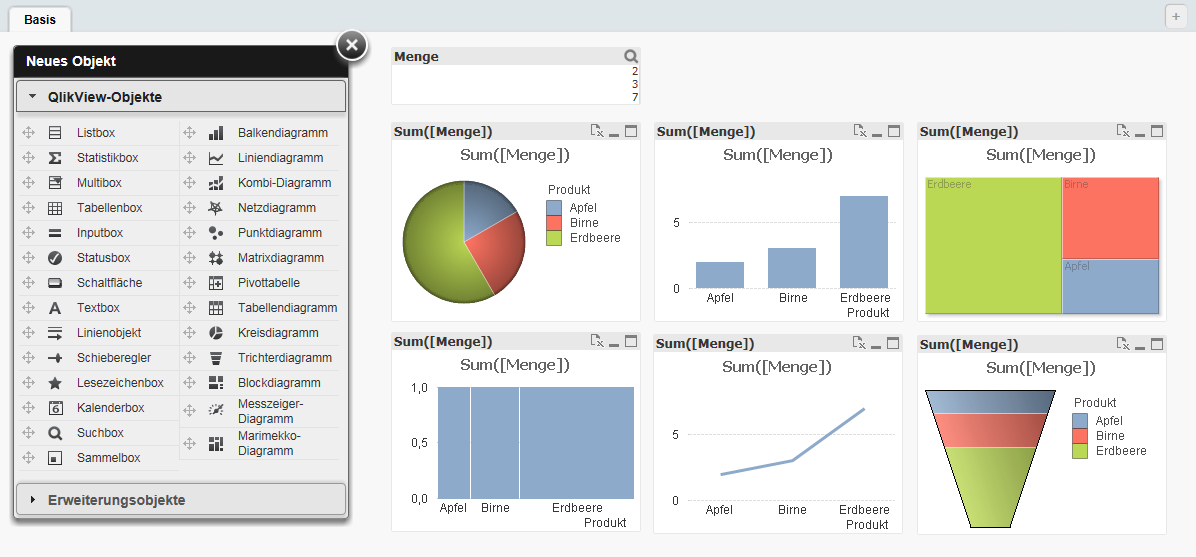
\includegraphics[width=0.95\textwidth]{img/QlikView/Sheet.png}
	\caption[Ein QlikView Sheet mit diversen Sheet Objects]{Ein QlikView Sheet mit diversen Sheet Objects, Quelle: Eigene Abbildung}
	\label{fig:Sheet}
\end{figure}


Ändert sich die Selektion der Daten, werden die Diagramme neu generiert, wie in Abbildung \ref{fig:SheetWithSelection} auf Seite \pageref{fig:SheetWithSelection} zu sehen ist. Nachdem zwei Datensätze ausgewählt wurden, zeigen die Diagramme ausschließlich die Daten der ausgewählten Selektion an.


\begin{figure}[htbp]
	\centering
		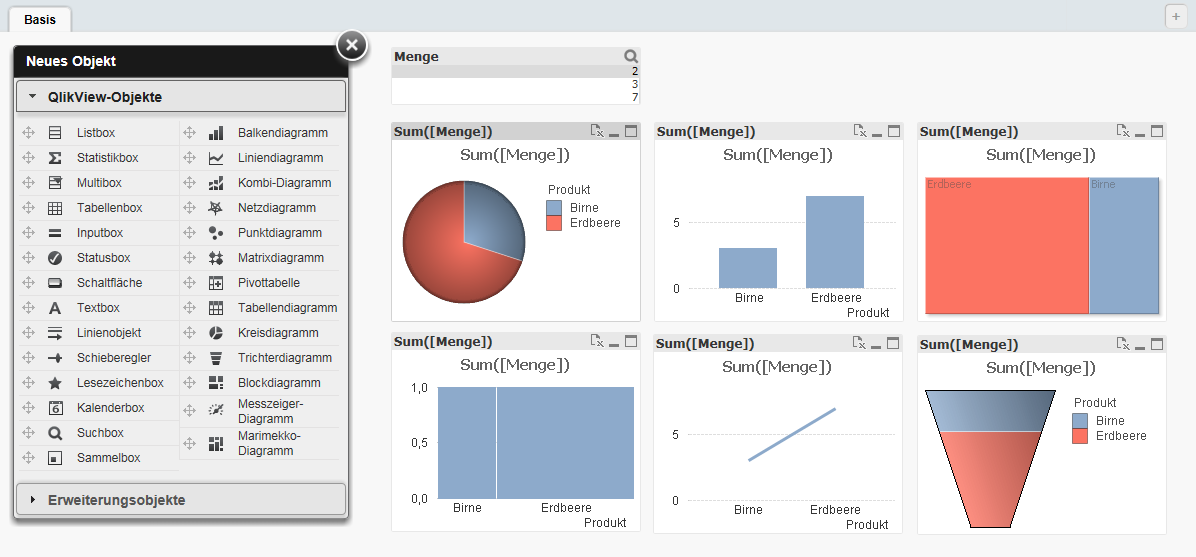
\includegraphics[width=0.95\textwidth]{img/QlikView/SheetWithSelection.png}
	\caption[Ein QlikView Sheet mit diversen Sheet Objects mit aktivierter Selektion]{Ein QlikView Sheet mit diversen Sheet Objects mit aktivierter Selektion, Quelle: Eigene Abbildung}
	\label{fig:SheetWithSelection}
\end{figure}

In QlikView erstellte Dokumente können über die Anzeige in einem Webbrowser auf unterschiedlichen Geräten dargestellt werden. Die Sheet Objects sind allerdings absolut positioniert und passen sich daher nicht der Größe des Displays an.

\newpage
\paragraph{Qlik Sense}
Qlik Sense ist eine weitere Business Intelligence Software der Firma, die sich mittlerweile in Qlik umbenannt hat.\footnote{Vgl. \cite{Qlik}} Die Software ähnelt QlikView in vielerlei Hinsicht, ist jedoch leichter zu bedienen und wurde für die Anzeige auf Geräten verschiedenster Größe vorbereitet. In Qlik Sense werden die Sheet Objects in einem Raster eingepasst. Das Raster füllt immer den zum Zeichnen verfügbaren Bereich aus.\footnote{Vgl. \cite[S. 11]{o2014qlik}}

Abbildung \ref{fig:SheetInSense} zeigt ein Arbeitsblatt in Qlik Sense, in der ähnliche Sheet Objects zum Einsatz kommen wie bereits in Abbildung \ref{fig:Sheet}. Einige der in QlikView verfügbaren Sheet Objects existierten jedoch zum Zeitpunkt der Erstellung der vorliegenden Arbeit nicht in Qlik Sense. In der Liste im linken Bereich der Abbildung erscheinen Sheet Objects sowie Extension Objects gleichermaßen und werden nicht wie in QlikView kategorisiert.

\begin{figure}[htbp]
	\centering
		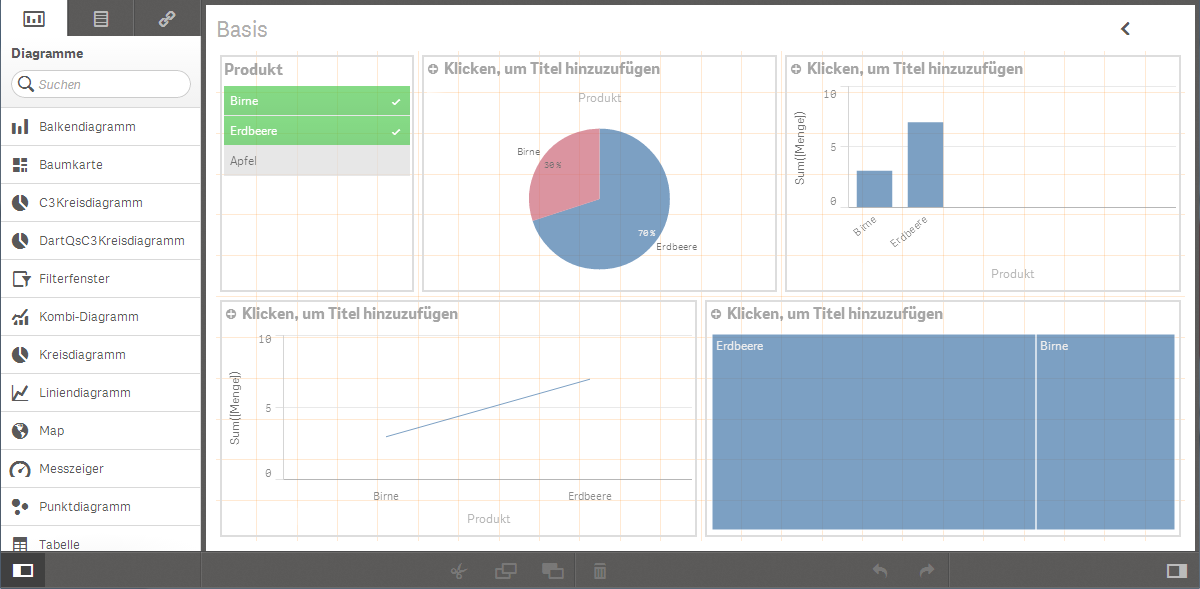
\includegraphics[width=0.95\textwidth]{img/QlikView/SheetInSense.png}
	\caption[Ein Qlik Sense Arbeitsblatt mit diversen Sheet Objects mit aktivierter Selektion]{Ein Qlik Sense Arbeitsblatt mit diversen Sheet Objects mit aktivierter Selektion, Quelle: Eigene Abbildung}
	\label{fig:SheetInSense}
\end{figure}






\subsection{Extension Objects und Document Extensions in QlikView}
% Kapitel richtet sich auch an Dart entwickler

QlikView verfügt bereits über eine Reihe von Diagrammtypen. Spezielle Anforderungen an die Anwendung erfordern jedoch auch speziellere Diagramme. Daher gibt es Bedarf nach neuen Diagrammtypen, die für einen individuellen Anwendungs\-fall benötigt werden, jedoch aufgrund ihrer Individualität nicht in QlikView integriert werden können. Zu diesem Zweck wurden in der Version 10 von QlikView die Extension Objects eingeführt.\footnote{Vgl. \cite[S. 163]{redmond2013qlikview}}

Diese Erweiterungen können genau wie die herkömmlichen Sheet Objects im Dokument frei positioniert und skaliert werden. Sie können Daten vom Server anfordern und sie mithilfe von Webtechnologien wie HTML, SVG, CSS und JavaScript beliebig visualisieren.
Eine weitere Möglich\-keit QlikView zu erweitern stellen die Document Extensions dar, die in der Version 11 von QlikView hinzugefügt wurden.\footnote{Vgl. \cite[S. 164]{redmond2013qlikview}} Anders als die Extension Objects handelt es sich hier nicht um positionierbare Objekte im Dokument, sondern um Erweiterungen des Dokumentes an sich. So kann beispielsweise mit den Document Extensions die Darstellung des Dokumentes angepasst werden.

In den weiteren Ausführungen dieses Kapitels wird beschrieben, wie Extension Objects und Document Extensions aufgebaut sind, wie sie erstellt und installiert werden, welche Nachteile Extension Objects in QlikView gegenüber den Sheet Objects haben und wie sich Extension Objects und Document Extensions auf die Performance auswirken.



\subsubsection{Struktur der Extension Objects und Document Extensions}

Extension Objects und Document Extensions in QlikView sind sich in ihrer Struktur sehr ähnlich. Sie haben beide eine \textit{Definition.xml}-Datei, in der beispielsweise Name und Typ definiert werden, und eine \textit{Skript.js}-Datei, in der das Verhalten der Erweiterung programmiert werden kann. Extension Objects haben darüber hinaus noch eine \textit{Properties.qvpp}-Datei, in welcher der Konfigurations\-dialog beschrieben wird, und eine \textit{Icon.png}-Datei, die als Vorschaubild in der Liste der verfügbaren Extension Objects angezeigt wird. Beide Dateien werden bei der Erstellung von Document Extensions ignoriert, da es keinen Konfigurations\-dialog und auch keine Liste verfügbarer Document Extensions gibt, in der ein Vorschaubild auftauchen könnte.

Im Nachfolgenden wird beschrieben, welche Funktion die einzelnen Dateien haben. 

\paragraph{Definition.xml}

Die \textit{Definition.xml}-Datei bestimmt die grundlegende Konfiguration des Extension Objects bzw. der Document Extension. Der Name, der Datei\-pfad und der Typ (Extension Object oder Document Extension) werden hier definiert. In der \textit{Definition.xml}-Datei wird die Anzahl der von dem Extension Object verwendeten Dimensionen und Formeln festgelegt. Außerdem müssen benutzerdefinierte Parameter in dieser Datei beschrieben werden. Zu guter Letzt können noch Startwerte für die Dimensionen, Formeln und benutzerdefinierten Parameter festgelegt werden.

In Abbildung \ref{fig:DefUndIcon2} auf Seite \pageref{fig:DefUndIcon2} ist unter anderem der Inhalt der Definition.xml-Datei zu sehen.

Der Wurzelknoten ist bei Document Extensions und Extension Objects gleich und lautet \textit{ExtensionObject}. Um festzulegen, dass es sich um eine Document Extension handelt, wird dem Knoten das Attribut \textit{Type} mit dem Wert \textit{document} zugewiesen. Für Extension Objects ist das Attribut optional, kann jedoch mit dem Wert \textit{object} gesetzt werden.\footnote{Vgl. \cite{ExtensionDefinitionFileQlikCommunity}}

Das Attribut \textit{Label} speichert die Bezeichnung von dem Extension Object. Diese taucht in der Liste der Extension Objects auf.

Für Document Extensions hat das Vergeben des Attributes \textit{Label} jedoch keinen Zweck. In der Dokumentation gibt es keinen Hinweis darauf, für welchen Typ von Erweiterungen das Attribut \textit{Label} verwendet werden kann und somit auch nicht darauf, dass es für Document Extensions keinen Effekt hat. Viele der im Internet öffentlich verfügbaren Document Extensions verwenden möglicherweise aus diesem Grund das Attribut dennoch, darunter die \textit{qvAutoRefresh} Document Extension\footnote{Vgl. \cite{qvAutoRefreshDefinitionXml}}. In der Liste der Document Extensions tauchen die Erweiterungen lediglich über den Datei\-pfad auf. In der Abbildung \ref{fig:DocumentExtensionListe} im Anhang \ref{lab:ScreenshotsVonQlikView} ist dies zu sehen. Statt dem Wert \textit{Inhalt Label} des Attributes \textit{Label} wird hier der Name des Ordners \textit{DocumentExtensionExample} angezeigt. In der Erweiterung \textit{DocumentExtensionWithoutLabel} wurde das Attribut \textit{Label} nicht gesetzt und taucht dennoch in der Liste auf.

Es ist auch möglich das Attribut \textit{Label} für Extension Objects zu entfernen, ohne eine Fehler\-meldung erwarten zu müssen. Ist das Attribut nicht auffindbar, so wird bei der Bezeich\-nung statt des Inhalts dieses Attributs wiederum der Ordnername angezeigt.

In dem Attribut \textit{Description} kann ein Beschreibungs\-text hinterlegt werden. Er taucht für eine Document Extension in dem Dialog für die Eigenschaften des Dokuments im Reiter \textit{Erweiterungen} in dem Textfeld \textit{Beschreibung der Erweiterung:} auf, wenn die Erweiterung in der Liste angewählt wurde. Für ein Extension Object steht der Beschreibungs\-text in der Kurzinfo. Die Kurzinfo wird angezeigt, wenn der Mauszeiger in der Liste der verfügbaren Extension Objects über die gewünschte Erweiterung bewegt wird.


\begin{figure}[htbp]
	\centering
		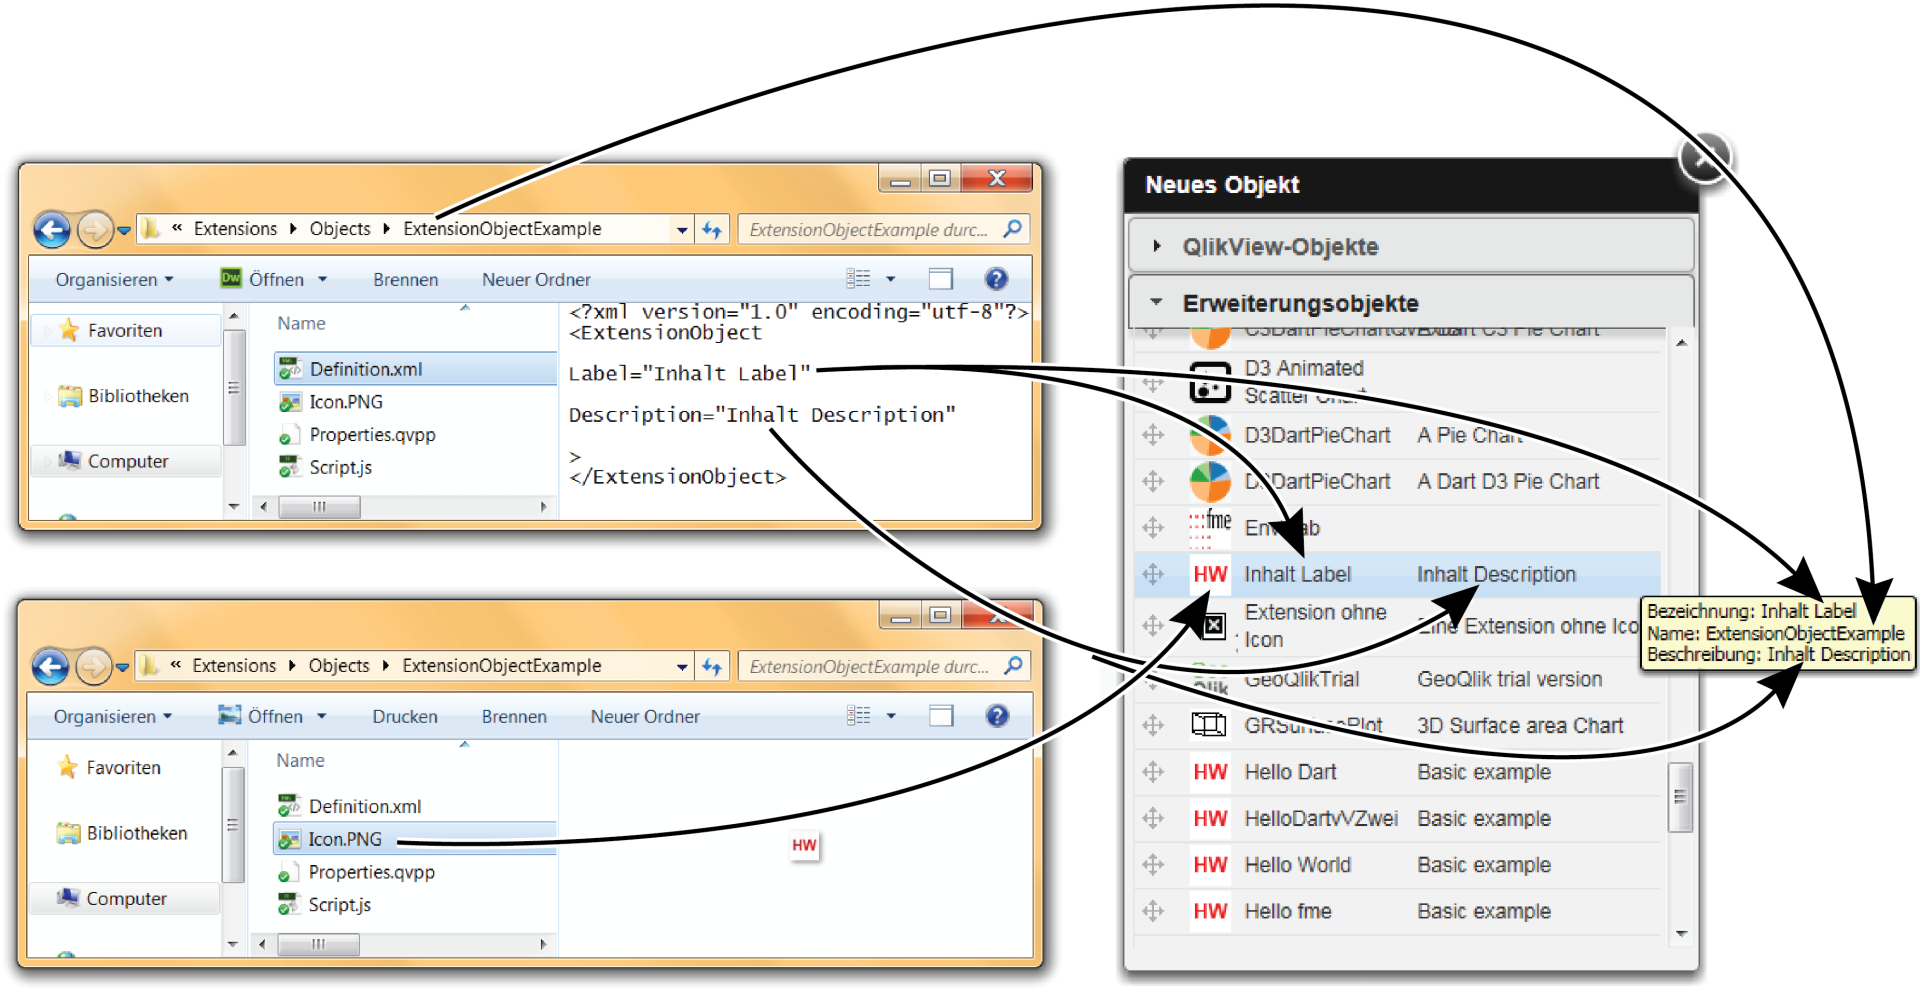
\includegraphics[width=1.00\textwidth]{./img/DefUndIcon/DefUndIcon2.png}
	\caption[Liste der verfügbaren Extension Objects]{Liste der verfügbaren Extension Objects mit der Visualisierung der Herkunft des Namens, der Bezeichnung, der Beschreibung und des Vorschaubildes, \\Quelle: Eigene Abbildung}
	\label{fig:DefUndIcon2}
\end{figure}

Alternativ kann auch das Attribut \textit{Path} zugewiesen werden. Der dort eingetragene Wert wird in der Kurzinfo für die Extension unter \textit{Name} angezeigt. Das Setzen des Attributes ist jedoch nicht notwendig, da hier der Name des Ordners, in dem die Extension gespeichert ist, eingetragen werden muss. Stimmt der Wert des Attributes nicht exakt mit dem Ordnernamen überein, so wird die Extension nicht in der Liste der verfügbaren Extensions auftauchen. Ist das Attribut einfach nicht vorhanden, so taucht der Ordnername ganz automatisch in dem Feld \textit{Name} der Kurzinfo auf. Die weniger redundante und sichere Methode ist es also, das Attribut bei der Erstellung der Datei einfach auszulassen.




\paragraph{Properties.qvpp}
\label{lab:PropertiesQvpp} 

Ab der Version QlikView 11 ist es möglich, das Erscheinungs\-bild des Dialoges für die Konfiguration des Extension Objects nach den Wünschen des Anwenders anzupassen. Zu diesem Zweck wird die automatische Generierung des Dialoges deaktiviert, wenn eine \textit{Properties.qvpp}-Datei im Ordner des Extension Objects vorhanden ist. In der Datei wird mittels HTML und CSS die visuelle Darstellung des Dialoges und seiner Eingabefelder beschrieben.\footnote{Vgl. \cite{QlikViewPropertiesPages}}

Für Document Extensions gibt es keinen Dialog für die Konfiguration, daher kann die \textit{Properties.qvpp}-Datei für diesen Anwendungs\-fall ignoriert werden.

\paragraph{Script.js}

In der \textit{Script.js}-Datei befindet sich der JavaScript-Code, der das Verhalten des Extension Objects bzw. der Document Extension steuert. Dies erfolgt durch Aufrufen von Funktionen der QlikView Ajax API. Sie ermöglichen die Interaktion der Erweiterung mit der QlikView Engine. So wird beispielsweise die Funktion \textit{AddExtension} verwendet, um ein Extension Object zu registrieren. Ihr werden der Name der Erweiterung sowie eine Funktion übergeben.\footnote{Vgl. \cite{QlikViewAjaxJavaScriptLibraryAddExtension}} Nach der Registrierung wird diese Funktion unter anderem immer dann aufgerufen, wenn die Erweiterung auf dem Sheet positioniert wird oder die Engine eine Veränderung der Selektion durch den Benutzer erkennt.



% XXX Ergänzen mit Infos zu den wichtigen Funktionen?
% XXX typische Fehler beim Umgang mit den Funktionen
% XXX Screenshots vom zugemüllten head element
% XXX Referenz von Stefan Walter

\newpage
\paragraph{Icon.png}

Die Icon.png-Bild\-datei repräsentiert das Vorschaubild der Extension. Es ist nur für Object Extensions verfügbar, da es für Document Extensions keinen Auswahldialog gibt, in dem Vorschaubilder angezeigt werden. Das Bild kann eine Auflösung von 24 × 24 Pixeln haben. Es wird in der Liste der verfügbaren Extension Objects angezeigt. Sollte die Datei nicht in demselben Ordner zu finden sein, in dem sich auch die Extension befindet, so wird statt des Vorschau\-bildes ein Fehler\-hinweis angezeigt. Dies ist in der Abbildung \ref{fig:OhneIcon} zu sehen.

\begin{figure}[htbp]
	\centering
		
\includegraphics[width=1.00\textwidth]{img/OhneIcon/OhneIcon.png}
	\caption[Fehlerhinweis für ein nicht auffindbares Vorschaubild eines Extension Objects]{Fehlerhinweis für ein nicht auffindbares Vorschaubild eines Extension Objects, Quelle: Eigene Abbildung}
	\label{fig:OhneIcon}
\end{figure}


\subsubsection{Installation von Extension Objects und Document Extensions}

Extension Objects und Document Extensions lassen sich auf die gleiche Art und Weise installieren. Für den QlikView Desktop Client gibt es dafür zwei Möglich\-keiten, für die Installation auf dem QlikView Server gibt es eine.
Die Installations\-methode, die für beide Technologien anwendbar ist, funktioniert folgendermaßen: Der Ordner, welcher den Namen des Extension Objects bzw. der Document Extension trägt und die benötigten Dateien enthält, wird dazu in ein spezielles Verzeichnis kopiert. Es befindet sich für den QlikView Desktop Client und für den QlikView Server an jeweils unterschiedlichen Orten. Für den QlikView Desktop Client ist der Pfad \textit{\%UserProfile\%\textbackslash{}AppData\textbackslash{}Local\textbackslash{}QlikTech\textbackslash{}QlikView\textbackslash{}Extensions\textbackslash{}Objects}.\footnote{Vgl. \cite[S. 164]{redmond2013qlikview}}

Sollte der Benutzername der Windows-Anmeldung beispielsweise \textit{user1} und der Datenträger, auf dem die Daten des Benutzers gespeichert sind, das Laufwerk \textit{C} sein, so wäre der Pfad \textit{C:\textbackslash{}Users\textbackslash{}user1\textbackslash{}AppData\textbackslash{}Local\textbackslash{}QlikTech\textbackslash{}QlikView\textbackslash{}Extensions\textbackslash{}Objects}.

Für den QlikView Server ist der Pfad \textit{\%ProgramData\%\textbackslash{}QlikTech\textbackslash{}QlikViewServer\textbackslash{}Extensions""\textbackslash{}Objects}.\footnote{Vgl. \cite[S. 164]{redmond2013qlikview}} 

Sollte sich der Ordner \textit{ProgramData} auf dem Laufwerk \textit{C} befinden, so ist der absolute Pfad \textit{C:\textbackslash{}ProgramData\textbackslash{}QlikTech\textbackslash{}QlikViewServer\textbackslash{}Extensions\textbackslash{}Objects}.

Nach dem Kopieren des Ordners ist die Installation bereits vollzogen.

Für den QlikView Desktop Client gibt es eine weitere Möglich\-keit, in der die Lokalisation des Ordners für die Erweiterungen erspart bleibt. Diese Option ist besonders für die Bereitstellung auf dem Zielrechner geeignet, da die Installation sehr einfach auch durch einen Laien mit einem Doppelklick erfolgen kann. Dazu wird der Ordner, der die Daten der Erweiterung enthält, in ein ZIP-Archiv gespeichert. Anschließend wird die Datei\-endung \textit{.zip} durch \textit{.qar} ersetzt. Sollte der QlikView Desktop auf dem Zielrechner verfügbar sein, muss die Datei auf dem Rechner lediglich ausgeführt werden, beispielsweise durch einen Doppelklick. Dabei werden die Ordner der Erweiterungen völlig automatisch in den korrekten Pfad kopiert.


\subsubsection{Nachteile von Extension Objects gegenüber Sheet Objects}
\label{lab:NachteileVonExtensionObjectsGegenüberSheetObjects} 

Einige der Funktionen, die in QlikView für die Sheet Objects zur Verfügung stehen, sind nicht für Extension Objects verfügbar.
% In Qlik Sense wurden diese Funktionen auch den Extension Objects hinzugefügt. Lesen Sie dazu das Kapitel XXX Kapitel einfügen XXX.
Eine sehr nützliche Funktion in QlikView sind die Dimension Limits. Sie sind in den Eigenschaften des Diagramms zu finden, welche sich über einen Rechtsklick auf das Diagramm und der Auswahl des Eintrages \textit{Eigenschaften…} aufrufen lassen. In der deutschen Version sind die Dimension Limits unter dem Reiter \textit{Beschränkung} zu finden. Die Dimension Limits erlauben die anzuzeigenden Daten zu beschränken und bieten sich vor allem dann an, wenn die Anzahl der Daten das Diagramm unübersichtlich werden lässt. Der Benutzer kann die anzuzeigenden Werte auf eine fixe Anzahl beschränken oder alternativ nur Werte anzeigen lassen, die eine vom Benutzer definierte Bedingung erfüllen. Alle sonstigen Daten können auf Wunsch unter einer beliebigen Bezeichnung zusammengefasst werden. Für Extension Objects in QlikView gibt es eine solche Funktion zur Begrenzung von Werten nicht. Lediglich durch eine eigene Implementation im Skript des Extension Objects kann eine solche Funktionalität hinzugefügt werden. 
% XXX Kapitel einfügen XXX
% XXX auf Beispiel verweisen? XXX

% XXX Colors?

\subsubsection{Erschwerte Fehlersuche durch das Fehlen von Entwicklerwerkzeugen}
\label{lab:ErschwerteFehlersucheDurchFehlenVonEntwicklerwerkzeugen} 

Der QlikView Desktop Client hat ausschließlich die Möglich\-keit über den sogenannten \textit{WebView} den Sheet in einer webbasierten Ansicht anzuzeigen. In der herkömmlichen Anzeige werden Extension Objects nicht dargestellt.\footnote{Vgl. \cite[S. 164]{redmond2013qlikview}}

Der integrierte \textit{WebView} hat keine Entwickler\-werkzeuge und nicht einmal eine JavaScript-Konsole ist vorhanden. Das Einsehen von Log- und Fehler-Ausgaben des Skriptes ist daher nicht möglich. Lediglich ein Extension Object mit dem Namen \textit{QvConsole} kann verwendet werden, um eine JavaScript-Konsole im Sheet darzustellen.\footnote{Vgl. \cite{walther2013comprehensive}} Doch dies ersetzt nicht die Entwickler\-werkzeuge eines Browsers, denn das Erstellen von Haltepunkten und Einsehen von Werten der Variablen ist damit nicht möglich. Dies erschwert die Fehler\-suche enorm.

Die einzige Möglich\-keit ist, die Anwendung auf einem QlikView Server auszuführen. Dann lässt sich das Dokument auch im Webbrowser öffnen und somit ist auch eine Fehler\-suche mithilfe der Entwickler\-werkzeuge des Browsers einfach möglich. Doch der QlikView Server ist nicht kostenfrei.\footnote{Vgl. \cite[S. 16 f.]{redmond2014qlikview}} Außerdem erfordert es deutlich mehr Aufwand ein QlikView-Dokument auf dem QlikView Server zu öffnen als im Desktop Client. Für das Dokument muss mithilfe der \textit{QlikView Management Console} zunächst ein sogenannter \textit{Task} erstellt werden, um es bereitzustellen.\footnote{Vgl. \cite[S. 111 ff.]{redmond2014qlikview}}

\newpage
\subsubsection{Auswirkungen auf die Performance}

Wird eine QlikView-Anwendung mit dem Browser geöffnet, werden die anzuzeigenden Diagramme von dem QlikView Server berechnet und als PNG-Datei an den Client übertragen. Damit liegt nicht nur der Großteil der Rechenlast auf dem Server, sondern auch die Aus\-last\-ung des Netzwerkes ist erhöht. Zudem muss jede Interaktion des Nutzers an den Server kommuniziert werden. Dazu gehört auch das Bewegen des Mauszeigers über einen Bereich im Diagramm. Dabei wird die Koordinate der Maus relativ zum Diagramm an den Server geschickt. Der Server berechnet, in welchem Bereich des Diagramms die Maus positioniert wurde und sendet die dazugehörigen Informationen an den Client zurück. Auf diese Weise werden in QlikView die Kurzinfos realisiert.

Extension Objects sowie Document Extensions verhalten sich anders. Sie werden mithilfe von Webtechnologien erstellt, die auf dem Webbrowser des Clients zur Ausführung gebracht werden. Die Rechenleistung wird damit auf dem Rechner des Clients beansprucht. Die Interaktion des Nutzers mit einem Extension Object wird nicht mehr zum Server übertragen, sondern kann direkt durch das dem Extension Object beigelegten Skript verarbeitet werden. Die anzuzeigenden Visualisierungen können mithilfe von dafür konzipierten Bibliotheken wie beispielsweise D3 erstellt und müssen so nicht über das Netzwerk übertragen werden. Ausschließlich die anzuzeigenden Daten, die durch das Extension Object dargestellt werden sollen, müssen an den Client gesendet werden.

\paragraph{Fazit}

Extension Objects und Document Extensions haben keinen negativen Einfluss auf die Ausführungs\-geschwindig\-keit des QlikView Servers, da lediglich die Rechenleistung des Clientrechners beansprucht wird. Darüber hinaus kann davon ausgegangen werden, dass Extension Objects die Ausführungs\-geschwindig\-keit sogar positiv beeinflussen können, wenn sie das Zeichnen der Diagramme auf dem Client Rechner ausführen, somit den Server entlasten und die Menge der über das Netzwerk zu übertragenden Daten verringern.










\subsection{Extension Objects in Qlik Sense}
Die Integration von Extension Objects in Qlik Sense ist deutlich besser, als dies noch in QlikView der Fall war. Qlik Sense verwendet die Technologien AngularJS und RequireJS, was die Entwicklung von Erweiterungen deutlich vereinfacht.\footnote{Vgl. \cite{ThirdPartySoftwareAttributionsCopyrightsLicensesAndDisclosure}} Dieses Kapitel beschreibt, welche Vorteile der neue webbasierte Ansatz bietet, welche Struktur Extension Objects in Qlik Sense haben und wie sie sich von den Sheet Objects unterscheiden. Weiterhin wird die Erstellung bzw. Installation von Extension Objects über das Datei\-system bzw. über die Qlik Sense Workbench erläutert.

\subsubsection{Webbasierte Anzeige und Entwicklerwerkzeuge}

Wie in Kapitel \ref{lab:ErschwerteFehlersucheDurchFehlenVonEntwicklerwerkzeugen} beschrieben, ist in QlikView die Fehler\-suche durch das Fehlen von Entwickler\-werkzeugen im \textit{WebView} deutlich erschwert.

In Qlik Sense ist dies nicht mehr der Fall, denn die Anzeige im QlikView Desktop Client wird über einen integrierten Chromium Browser realisiert.\footnote{Vgl. \cite[o. S.]{QlikSenseArchitecture}} Mit der Tasten\-kombination \textit{Steuerung} + \textit{Shift} + \textit{Rechtsklick} im Fenster des Qlik Sense Desktop Clients öffnet sich ein Dialog, in dem über den Eintrag \textit{Show DevTools} die Entwickler\-werkzeuge geöffnet werden können. Ist Qlik Sense gestartet, ist es jedoch auch möglich mit jedem anderen modernen Webbrowser über die Adresse \url{http://localhost:4848/hub/} den Qlik Sense Desktop-Hub zu öffnen.\footnote{Vgl. \cite[o. S.]{QlikSenseArchitecture}}

\subsubsection{RequireJS}

In der Vorgängerversion QlikView wurde das Anfordern von weiteren Dateien noch über herkömmliche Ajax-Anfragen über absolute Adressen realisiert.\footnote{Vgl. \cite{QlikViewAjaxJavaScriptLibraryLoadExtensionScripts}} Qlik Sense verwendet dagegen eine Bibliothek für die Definition von Modulen. 

\begin{quote}
Qlik Sense uses RequireJS for loading JavaScript modules [...].\footnote{\cite{QlikSenseWorkbenchRequirementsAndAssumptions}}
\end{quote}

Die Bibliothek erlaubt es, JavaScript-Module mit ihren Abhängig\-keiten von anderen Modulen zu definieren.

\subsubsection{Extension Objects gleichen Sheet Objects}

In QlikView bestand noch ein klarer Unterschied zwischen Extension Objects und Sheet Objects - siehe Kapitel \ref{lab:NachteileVonExtensionObjectsGegenüberSheetObjects}. Allerdings ist es in Qlik Sense schwer, Unterschiede zwischen diesen beiden Kategorien festzustellen. Ein leicht zu erkennender Unterschied ist jedoch, dass die herkömmlichen Sheet Objects nicht im Datei\-ordner zu finden sind, in dem die Extension Objects abgelegt werden.

Während Qlik Sense ausgeführt wird und ein Arbeitsblatt im Webbrowser geöffnet ist, kann in der JavaScript-Konsole über den Ausdruck \textit{requirejs.s.contexts.\_.defined} eine Liste aller definierten Module ausgegeben werden.\footnote{Vgl. \cite{FiveHelpfulTipsWhenUsingRequireJSTechPro}} In der Liste tauchen unter anderem alle Extension Objects auf, die zum aktuellen Arbeitsblatt hinzugefügt wurden. So ist zum Beispiel auch das im Kapitel \ref{lab:LeitfadenZurErstellungEinesQlikSenseExtensionObjectsMitJavaScript} erstellte Kreisdiagramm in der Liste unter dem Eintrag \textit{extensions""/C3Kreisdiagramm""/C3Kreisdiagramm} zu finden. Sofern das durch Qlik Sense mitgelieferte Kreisdiagramm dem Arbeitsblatt ebenso zugewiesen ist, lässt sich auch der Eintrag \textit{extensions.qliktech""/piechart""/piearea} finden. Dies lässt vermuten, dass die mitgelieferten Sheet Objects sowie die Extension Objects die gleichen Technologien verwenden und somit kein Unterschied in ihrer Anwendung besteht. Die Nachteile der Extension Objects in QlikView, welche im Kapitel \ref{lab:NachteileVonExtensionObjectsGegenüberSheetObjects} erläutert wurden, existieren in Qlik Sense nicht. So ist es beispielsweise möglich, auch für Extension Objects in Qlik Sense Limitierungen für Dimensionen zu definieren.\footnote{Vgl. \cite[S. 89 ff.]{o2014qlik}}

\subsubsection{Qlik Sense Workbench}
\label{lab:QlikSenseWorkbench} 

Ist Qlik Sense Desktop installiert und gestartet, so lässt sich über die URL \url{localhost:4848/workbench/} die Qlik Sense Workbench aufrufen.\footnote{Vgl. \cite{QlikSenseWorkbench,LaunchingQlikSenseWorkbench, QlikTipsExtensionsInQlikSense}} Im Anhang \ref{lab:ScreenshotsVonQlikSense} in Abbildung \ref{fig:Workbench} ist ein Screenshot der Workbench zu sehen. Über die Schaltfläche \textit{Create New} kann ein neues Extension Object oder auch ein neues Mashup - diese werden in der vorliegenden Arbeit nicht erläutert - erstellt werden.
Die Workbench erzeugt mithilfe von Schablonen alle benötigten Dateien selbstständig. Der Entwickler kann die Dateien direkt im Anschluss innerhalb der Workbench editieren.

\subsubsection{Qlik Sense Extension Objects auf dem Dateisystem}

Wird eine Erweiterung über die Qlik Sense Workbench erstellt, so tauchen die generierten Dateien im Datei\-system unter \textit{\%UserProfile\%\textbackslash{}Documents\textbackslash{}Qlik\textbackslash{}Sense\textbackslash{}Extensions} auf.\footnote{Vgl. \cite{QlikTipsExtensionsInQlikSense}}

Wenn der Benutzername der Windows-Anmeldung \textit{user1} und die Daten des Benutzerkontos auf dem Laufwerk C gespeichert sind, dann ist der Pfad \textit{C:\textbackslash{}Users""\textbackslash{}user1""\textbackslash{}Documents""\textbackslash{}Qlik""\textbackslash{}Sense""\textbackslash{}Extensions}.


Für die Erstellung der Dateien muss nicht zwingend die Qlik Sense Workbench verwendet werden. Sie können auch unabhängig von der Workbench durch beliebige Programme erstellt und modifiziert werden.

\subsubsection{Struktur von Qlik Sense Extension Objects}

Die beiden wichtigsten Dateien sind die \textit{.qext}-Datei und die \textit{.js}-Datei. Als Datei\-namen erhalten beide den exakten Namen des Extension Objects. Weiterhin gibt es eine \textit{wbfolder.wbl}-Datei, welche optional ist. Darüber hinaus können beliebig viele weitere Dateien hinzugefügt werden, die für das Skript verwendet werden sollen. Die Dateien erfüllen unterschiedliche Funktionen.

\paragraph{.qext-Datei}

Der Inhalt der \textit{.qext}-Datei ist im JSON-Format beschrieben und speichert grundlegende Informationen des Extension Objects.\footnote{Vgl. \cite{QlikTipsExtensionsInQlikSense}} Dazu gehören unter anderem der Name, die Beschreibung, der Typ oder aber ein Vorschaubild. In der Liste der verfügbaren Extension Objects tauchen diese Informationen entweder direkt in der Liste oder in einer Kurzinfo nach dem Klick auf einen der Einträge auf.

\paragraph{.js-Datei}

Der Haupteinstiegspunkt des Skriptes befindet sich in der Datei mit dem Namen der Erweiterung und der Endung \textit{.js}.\footnote{Vgl. \cite{QlikTipsExtensionsInQlikSense}} Anders als in QlikView kann die Definition der Dimensionen, der Formeln, der Parameter und deren Eingabefelder vollständig in dieser Datei erfolgen. Alternativ können auch weitere Module angelegt werden, die das RequireJS-Skript anfordert.

\paragraph{wbfolder.wbl-Datei}


Bei der \textit{wbfolder.wbl}-Datei handelt es sich um eine Liste der zu dieser Erweiterung gehörenden Dateien. Sie hat den Zweck, die Reiter in der Qlik Sense Workbench zu verwalten. Außerdem werden beim Duplizieren der Erweiterung innerhalb der Workbench ausschließlich die Dateien, die in dieser Liste eingetragen sind, kopiert. Alle anderen Dateien werden ignoriert.


\subsection{Die Programmiersprache Dart}




\subsubsection{Allgemeines zur Programmiersprache Dart}

Dart ist eine durch Google entwickelte Programmiersprache für die Entwicklung von komplexen und zugleich hochperformanten Webapplikationen. Die Sprache wurde entwickelt, da aus der Sicht von Google die Etablierung einer weiteren Sprache neben JavaScript für die Webentwicklung nötig war.

\begin{quote}
JavaScript is great for small scripts, and it has the performance chops to run large apps. But when a script evolves into a large web app, debugging and modifying that app can be a nightmare, especially when you have a large team.\footnote{Vgl. \cite[S. 1]{walrath2012dart}}
\end{quote}

Ziel der Programmiersprache Dart war es unter anderem, Entwicklern, die mit Sprachen wie Java und C\# vertraut sind, die Programmierung für das Web zu ermöglichen. Gleichzeitig sollte der Einstieg für JavaScript-Entwickler dadurch nicht erschwert werden. Um dem zu begegnen, ist die Verwendung von Typen in Dart optional. Wie in JavaScript gewohnt, kann eine Variable mit dem Schlüssel\-wort \textit{var} deklariert werden. Gleichermaßen kann anstelle des \textit{var}-Schlüssel\-wortes auch ein Typ wie zum Beispiel \textit{String}, \textit{int} oder \textit{Object} stehen.\footnote{Vgl. \cite[S. 5]{buckett2013dart}}

Dart verfügte bereits zum Zeitpunkt der Standardisierung als ECMA-408 Standard um einige Konzepte, die aus anderen objekt\-orientierten Programmier\-sprachen wie beispielsweise C++, Java und C\# bekannt sind. Dazu gehören unter anderem Klassen, Interfaces, Mixins, Properties, generische Daten\-typen und Annotationen.\footnote{Vgl. \cite[o. S.]{EcmaDartProgrammingLanguageSpecificationFirstEdition}}

Darüber hinaus äußerte die Community weitere Wünsche nach Funktionalitäten, die in der Sprache noch nicht enthalten waren. So wurden beispielsweise Enum-Typen gewünscht, wie sie in Java, C\# und C++ vorkommen.\footnote{Vgl. \cite{EnhancementEnumDart}}
Ein weiterer Vorschlag war das Hinzufügen der Schlüsselwörter \textit{async} und \textit{await} für eine deutlich verbesserte Lesbar\-keit im Umgang mit asynchroner Programmierung.\footnote{Vgl. \cite{SupportForAwaitInDart}}

Das Dart-Entwicklerteam antwortete darauf und so wurden die gewünschten Funktionalitäten der zweiten Edition des Standards bereits sechs Monate nach der initialen Standardisierung hinzugefügt.\footnote{Vgl. \cite[S. 43, 88]{EcmaDartProgrammingLanguageSpecificationSecondEdition}}


\subsubsection{Kompilierbarkeit zu JavaScript}

Um Dart auch auf jedem modernen Webbrowser ausführen zu können, kann der Compiler dart2js verwendet werden. Er übersetzt den Dart-Quellcode, inklusive aller Abhängig\-keiten, in JavaScript. Auch nach der Kompilierung kann die Ausführungs\-geschwindig\-keit des generierten JavaScript-Codes schneller sein als eine äquivalente Implementierung in reinem JavaScript. Dies konnte durch Benchmarks, wie zum Beispiel dem sogenannten Tracer-Test, ermittelt werden.\footnote{Vgl. \cite[S. 2 f]{belchin2015advanced}}
Weitere Benchmarks sind auf folgender Webseite einsehbar: \url{dartlang.org/performance/}.

\subsubsection{Werkzeuge}

Für die Programmierung mit Dart wurde der Dart Editor geschaffen. Dabei handelt es sich um eine auf Eclipse basierende integrierte Entwicklungsumgebung. Der Editor unterstützt den Entwickler unter anderem mit statischer Quellcodeanalyse und Debuggingtools. Mithilfe von Plug-ins ist die Programmierung von Dart-Anwendungen auch innerhalb von anderen Entwicklungsumgebungen möglich. Es existieren Plug-ins für IntelliJ IDEA, WebStorm, Sublime Text 3, Emacs und Vim.\footnote{Vgl. \cite[o. S.]{akopkokhyants2014mastering}}

\subsubsection{Bibliotheken in Dart}

Dart ist nicht nur eine Programmiersprache, sondern vielmehr eine Plattform. Dart wird bereits mit einer Reihe von integrierten Bibliotheken ausgeliefert. Kollektionen, reguläre Ausdrücke, mathematische Operationen und die Interaktion mit dem DOM sind nur einige von den vielen Funktionen, die durch diese Bibliotheken abgedeckt werden.\footnote{Vgl. \cite[S. 4]{walrath2012dart}}

Sollte dennoch eine Bibliothek benötigt werden, so kann sie über den Paketmanager Pub angefordert werden. Er ermöglicht es, Abhängig\-keiten zu anderen Bibliotheken hinzuzufügen. Welche aus unterschiedlichen Quellen stammen können. Google selbst bietet einen Service an, solche sogenannten packages auf der Seite \url{pub.dartlang.org} zu hinterlegen. Alternativ kann auch ein git repository gewählt werden und natürlich lassen sich auch packages im lokalen Datei\-system ablegen und einbinden. Dart wird mit einem Kommando\-zeilen\-programm ausgeliefert, welches ebenfalls den Namen \textit{pub} trägt. Jedes Dart-Projekt enthält eine Datei mit dem Datei\-namen \textit{pubspec.yaml}. Darin werden alle Abhängig\-keiten gelistet, die durch den Paketmanager verwaltet werden sollen. Über den Befehl \textit{pub get} werden alle eingetragenen Abhängig\-keiten des Projektes aufgelöst und gegebenenfalls heruntergeladen. Dabei werden auch die Abhängig\-keiten der angeforderten packages ermittelt und ebenfalls hinzugefügt.\footnote{Vgl. \cite[S. 183]{kopec2014dart}}

\subsubsection{Build Tools}


Die Automatisierung immer wiederkehrender Aufgaben beim Entwicklungsprozess kann eine Zeit sparende Erleichterung sein. Die Anwendungsgebiete sind vielfältig. Beispiele sind das Durchlaufen von Modultests, die automatische Kompilierung von Sass-Quell\-dateien in CSS-Code oder die Verringerung der Datei\-größe der generierten Dateien.\footnote{Vgl. \cite[S. 391]{odell2014pro}} Doch es kann sich auch einfach um das Kopieren der generierten Dateien auf einen entfernten Server handeln. Dieses Szenario wird auch bei der Entwicklung der QlikView und Qlik Sense Erweiterungen mithilfe von Dart eine Rolle spielen. 
Für JavaScript existiert ein sogenanntes build tool mit dem Namen Grunt.\footnote{Vgl. \cite[S. 392]{odell2014pro}} Doch um dieses build tool zu verwenden, müssen Node.js und anschließend unterschiedliche Node.js packages installiert werden.\footnote{Vgl. \cite[S. 393]{odell2014pro}}

Dart bietet dagegen die sogenannten Pub Transformer als ein build tool an, welches ohne weitere Installation verwendet werden kann. Die gewünschten Transformer werden in der \textit{pubspec.yaml}-Datei angegeben und bei jedem Build-Prozess durch den Befehl \textit{pub build} automatisch angestoßen.\footnote{Vgl. \cite{AssetsAndTransformers}}

In den Kapiteln \ref{lab:TransformerZumAnpassenDerSourceMapsFürQlikViewErweiterungen} und \ref{lab:TransformerZurBereitstellungDerQlikViewUndQlikSenseErweiterungen}   ist die Anwendung der Pub Transformer zu sehen.












































\section{Vorbereitende Entwicklung von Erweiterungen mit \\JavaScript}
\label{lab:VorbereitendeEntwicklungVonErweiterungenMitJavaScript} 

In diesem Kapitel werden ein QlikView Extension Object und eine QlikView Document Extension sowie ein Qlik Sense Extension Object mit JavaScript erstellt. Es dient Entwicklern, die Extension Objects bzw. Document Extensions in JavaScript oder auch Dart entwickeln möchten, gleichermaßen, denn viele der Schritte sind identisch. Lediglich bei der Erstellung des Skriptes gibt es Unterschiede. Daher sollten auch Entwickler, die in die Extension Entwicklung mit Dart einsteigen möchten, sich über die Grundlagen der Entwicklung von Extension Objects und Document Extensions in diesem Kapitel vertraut machen.

\subsection{Leitfaden zur Erstellung eines QlikView Extension Objects mit \\JavaScript}
\label{lab:LeitfadenZurErstellungEinesExtensionObjectsMitJavaScript} 
% Ordner erstellen mitden Skripten dises Kapitels 

In diesem Kapitel wird die Entwicklung eines Extension Objects am Beispiel eines Kreis\-diagramms mit JavaScript erklärt. Um das Beispiel möglichst knappzuhalten und dennoch auf die wichtigen Details bei der Extension Erstellung einzugehen, wurde die Bibliothek C3 verwendet. Sie verwendet im Kern D3, welcher eine sehr flexible und funktionsreiche Bibliothek zur Visualisierung von Daten ist. C3 bietet eine Reihe von wiederverwendbaren Diagrammen, die mit einem verhältnismäßig geringen Entwicklungsaufwand verwendet und konfiguriert werden können.\footnote{Vgl. \cite{C3D3BasedReusableChartLibrary}}

\subsubsection{Besonderheiten}

In der Mitte der Abbildung \ref{fig:Vergleich} auf Seite \pageref{fig:Vergleich} ist das Kreisdiagramm in einem QlikView-Dokument dargestellt. Die selektierten Daten der links im Bild befindlichen ListBox werden durch das Kreisdiagramm visualisiert. Rechts im Bild ist zum Vergleich ein durch QlikView mitgeliefertes Kreisdiagramm zu sehen. Das Dokument wird im Browser mit einem angewendeten Zoom dargestellt. Das von QlikView mitgelieferte Kreisdiagramm erscheint durch die erkennbaren Rasterpunkte weniger ästhetisch. Die Darstellung des C3 Kreis\-diagramms wird nicht verschlechtert, da es sich um eine Vektorgrafik handelt.

\begin{figure}
	\centering
		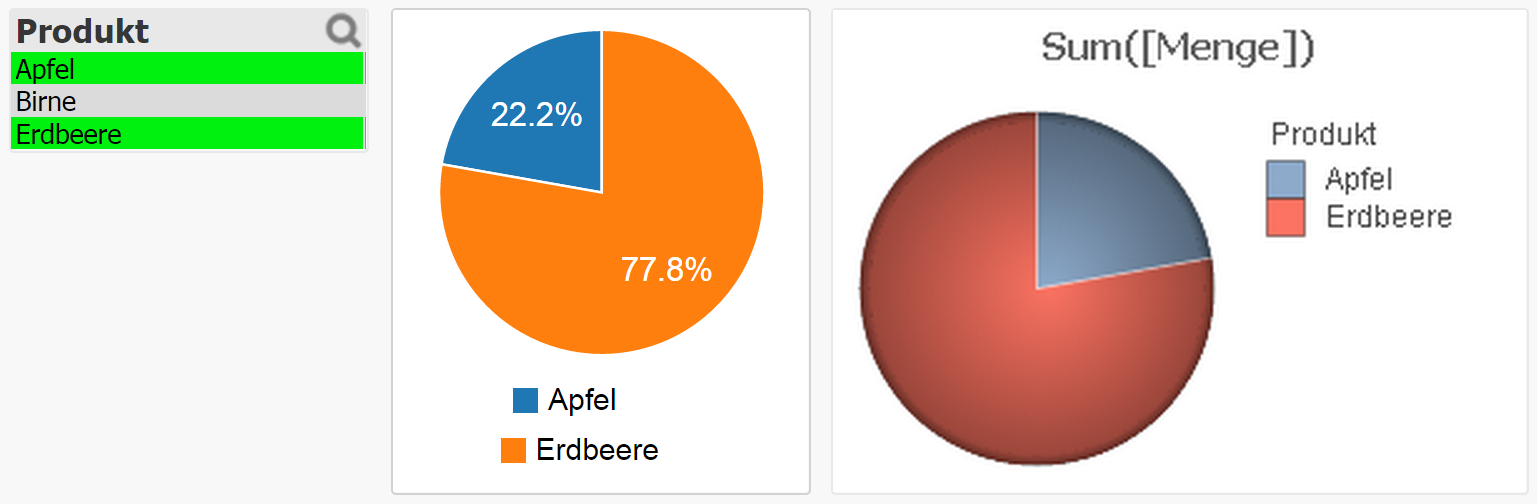
\includegraphics[width=1.00\textwidth]{img/KreisdiagrammScreenshot/Vergleich.PNG}
	\caption[Screenshot des C3 Kreisdiagramms]{Screenshot des C3 Kreisdiagramms - Mitte - sowie eines von QlikView mitgelieferten Kreisdiagramms - rechts, Quelle: Eigene Abbildung}
	\label{fig:Vergleich}
\end{figure}

\subsubsection{Erstellen der Dateistruktur}

Das Extension Object soll den Namen C3Kreisdiagramm erhalten. Daher erhält der Datei\-ordner genau diesen Ordner\-namen, da er den Namen des Extension Objects festlegt. Alle im Rahmen des Beispiels erstellten Dateien werden in diesem Ordner gespeichert. Weiterhin müssen die benötigten Dateien der Bibliotheken in diesen Ordner heruntergeladen werden. Die Dateien sind \textit{d3.min.js} \footnote{\url{https://github.com/mbostock/d3/blob/master/d3.min.js}}, \textit{c3.min.js} \footnote{\url{https://github.com/masayuki0812/c3/blob/master/c3.min.js}} und \textit{c3.min.css} \footnote{\url{https://github.com/masayuki0812/c3/blob/master/c3.min.css}}.

\subsubsection{Erstellen eines QlikView-Testdokumentes}
\label{lab:ErstellenEinesQlikViewTestdokumentes} 

Zur Visualisierung werden Daten benötigt. Weiterhin werden die Extension Objects bzw. die Document Extensions einem QlikView-Dokument zugewiesen. Daher muss zunächst ein Dokument im QlikView Desktop Client angefertigt werden. Für dieses Beispiel werden im QlikView load script Daten zum Test erstellt. Das Listing \ref{lst:InlineLoadFuerTestdaten} wird am Ende des Skriptes eingefügt. Es dient der Erzeugung von drei Daten\-sätzen, die für die Visualisierung verwendet werden können.

\begin{listing}[htbp]
\begin{minted}[mathescape,
               linenos,
               numbersep=5pt,							
							firstnumber=12,
               gobble=0,
               frame=lines,
							fontsize=\small,
               framesep=2mm]{javascript}
Produkte:
load * inline
[ Produkt, Menge,
  Apfel, 2,
  Birne, 3,
  Erdbeere, 7
];
\end{minted}
\caption[Inline Load für Testdaten]{Inline Load für Testdaten, \\Quellcode\textbackslash{}load script\textbackslash{}QlikView load script.txt, Quelle: Eigenes Listing}
\label{lst:InlineLoadFuerTestdaten}
\end{listing}

\subsubsection{Hinzufügen eines CSS-Stylesheet}
\label{lab:HinzufügenEinesCSSStylesheet}

Für die korrekte Darstellung des Kreis\-diagramms wird eine CSS-Anweisung benötigt. Sie ist im Listing \ref{lst:JavascriptC3KreisdiagrammCSSStylesheet} zu sehen und wird als Datei mit dem Namen \textit{style.css} im Ordner der Erweiterung abgelegt. Sie sorgt dafür, dass die generierte Vektorgrafik korrekt im zu zeichnenden Bereich erstellt wird. Fehlt die Anweisung, ist die generierte Vektorgrafik größer als der Bereich, welcher für die Erweiterung vorgesehen ist.

\begin{listing}[htbp]
\begin{minted}[mathescape,
               linenos,
               numbersep=5pt,
               gobble=0,				
               frame=lines,
							fontsize=\small,
               framesep=2mm]{css}
.kreisdiagramm { height: 100%; width: 100%; }
\end{minted}
\caption[\textit{style.css}-Datei des QlikView C3Kreisdiagramm Extension Objects]{\textit{style.css}-Datei des QlikView C3Kreisdiagramm Extension Objects, \\Quellcode\textbackslash{}JavaScript\textbackslash{}QlikView\textbackslash{}C3Kreisdiagramm\textbackslash{}style.css, \\Quelle: Eigenes Listing}
\label{lst:JavascriptC3KreisdiagrammCSSStylesheet}
\end{listing}

\subsubsection{Erstellung der Definition.xml-Datei}

In dem Listing \ref{lst:JavascriptC3KreisdiagrammDefinition} ist die \textit{Definition.xml}-Datei für das Extension Object zu sehen.


\begin{listing}[htbp]
\begin{minted}[mathescape,
               linenos,
               numbersep=5pt,
               gobble=0,
               frame=lines,
							fontsize=\small,
               framesep=2mm]{xml}
<?xml version="1.0" encoding="utf-8" ?>
<ExtensionObject Label="C3 Kreisdiagramm"
  Description="Ein simples Kreisdiagramm">

  <!-- Dimension 0 - Feld der anzuzeigenden Entitaeten im Kreisdiagramm -->
  <Dimension Initial="" />
  <!-- Formel 0 - Formel der anzuzeigenden Werte im Kreisdiagramm -->
  <Measurement Initial="" />
  <!-- Parameter 0 - Auswahlbox zum Festlegen der Anzeige der Legende. -->
  <Text Label="Show Legend" Type="checkbox" />

  <!-- Initialisiere Dimension 0 mit Produktname -->
  <Initiate Name="Chart.Dimension.0.Field" Value="Produkt" />
  <!-- Initialisiere Formel 0 mit Produktmenge -->
  <Initiate Name="Chart.Expression.0.0.Definition" Value="=Menge" />
  <!-- Initialisiere Parameter 0 (Legende) mit false -->
  <Initiate Name="Chart.Text.0.Content" Value="0" />

  <PropertiesPage Version="11" File="Properties.qvpp" />
</ExtensionObject>
\end{minted}
\caption[\textit{Definition.xml}-Datei des QlikView C3Kreisdiagramm Extension Objects]{\textit{Definition.xml}-Datei des QlikView C3Kreisdiagramm Extension Objects, \\Quellcode\textbackslash{}JavaScript\textbackslash{}QlikView\textbackslash{}C3Kreisdiagramm\textbackslash{}Definition.xml, \\Quelle: Eigenes Listing}
\label{lst:JavascriptC3KreisdiagrammDefinition}
\end{listing}
% = oder ohne?
% Initial="" bringt das was?

\paragraph{Dimensionen festlegen}

Das Kreisdiagramm soll genau eine Dimension visualisieren, in diesem Beispiel die Dimension \textit{Produkt}. In Zeile 6 wird die Dimension erstellt. Dafür kann keine Id festgelegt werden, denn die Dimensionen werden nach ihrer Reihenfolge des Auftretens in dieser Datei durchnummeriert. Die erste Dimension erhält deshalb die Referenz \textit{Chart.Dimension.0}, während eine weitere Deklaration einer Dimension die Referenz \textit{Chart.Dimension.1} erhalten würde.

Der Knoten Dimension enthält das Attribut \textit{Initial}, welches gesetzt werden muss. Ist das Attribut nicht auffindbar, so wird die Dimension nicht deklariert und somit ist sie in der Extension nicht verfügbar. Allerdings ist es aber auch unerheblich, welcher Wert dem Attribut hinzugefügt wird. Die für diese Arbeit durchgeführten Tests zeigten, dass dieses Attribut den Wert des Feldes nicht initialisiert. Es reicht aus, das Attribut zu deklarieren und ihm eine leere Zeichenkette als Wert zu übergeben. Das Initialisieren des Wertes der Dimension ist jedoch möglich und wird in der Zeile 13 mit dem Wert \textit{Produkt} vorgenommen.


\paragraph{Formeln festlegen}

In Zeile 8 erfolgt die Deklaration der Formel. Auch hier ist das Festlegen einer Id nicht möglich, sondern wird genau wie bei den Dimensionen über die Reihenfolge der Deklarationen in der Datei bestimmt. Allerdings gibt es hier einen Unterschied in der Syntax der Referenzierung. Die in der Zeile definierte Formel erhält die Referenz \textit{Chart.Expression.0.0}, während eine weitere Formel die Referenz \textit{Chart.Expression.1.0} erhalten würde. Die zweite Nummer scheint bei der Referenz immer eine \textit{0} zu sein. In Zeile 15 wird die Formel über die korrekte Referenz initialisiert. Zu jedem Daten\-satz soll die dazugehörige \textit{Menge} angezeigt werden.

\paragraph{Parameter festlegen}


Ob die Legende des Diagramms angezeigt wird, soll über einen Parameter, der in Zeile 10 definiert wird, konfigurierbar sein. Das Attribut \textit{Label} ist nur von Bedeutung, wenn der Konfigurations\-dialog automatisch generiert wird. Während der Entwicklung der Extension wird jedoch ein eigener Konfigurations\-dialog erstellt und somit ist das Attribut bedeutungslos. Das Attribut \textit{Type} legt fest, welche Art von Eingabefeld für den Parameter angewendet werden soll. In diesem Beispiel ist es \textit{checkbox}, da es sich um die Deklaration eines Wahrheits\-wertes handelt. 

Darüber hinaus gibt es weitere Typen von Eingabefeldern. Für Zeichenketten erhält das Attribut den Wert \textit{text}, für Farben den Wert \textit{color} und für eine Dropdown-Liste den Wert \textit{select}.\footnote{Vgl. \cite{ExtensionDefinitionFileQlikCommunity}}

Allerdings muss darauf hingewiesen werden, dass die Auswahlbox fehlerhaft ist. Damit die Dropdown-Liste verwendet werden kann, muss zusätzlicher Code zur JavaScript-Datei der Extension hinzugefügt werden.\footnote{Vgl. \cite{HTMLSelectInExtensionsQlikCommunity}}

Genau wie bei den Dimensionen und Formeln wird die Identifikation der Parameter über die Reihenfolge ihrer Definition in der Datei bestimmt. Die Referenz des ersten Parameters lautet \textit{Chart.Text.0}, während die des zweiten Parameters \textit{Chart.Text.1} wäre. In Zeile 17 wird der Wahrheits\-wert des Parameters mit der Nummer 0 - für unwahr - initialisiert. 
% Welches ist meine QLik View Version?

Das Festlegen eines Bezeichners für die Parameter wäre wünschenswert. Wird nämlich der erste Parameter entfernt, so werden auch die Identifikationsnummern wieder neu durch\-nummeriert. Wenn das passiert, müssen alle Parameter im Konfigurationsdialog, welcher in der \textit{Properties.qvpp}-Datei beschrieben wird, erneut verknüpft werden. Dort erhält der Parameter, welcher zuvor an zweiter Stelle war und nun auf die erste Stelle aufgerückt ist, die Referenz \textit{Chart.Text.0} statt vorher \textit{Chart.Text.1}. Ebenso müssen die Aufrufe der Parameter in der \textit{Script.js}-Datei angepasst werden. In dieser Datei erhält der Parameter, der zuvor der zweite Parameter war, nun die Referenz \textit{Layout.Text0} statt vorher \textit{Layout.Text1}. Dies wird mit einer zunehmenden Anzahl von Parametern immer mühsamer und verleitet dazu, so wenig Parameter wie möglich zu integrieren oder beim Löschen eines Parameters in der \textit{Definition.xml}-Datei die Lücke der Identifikationsnummern durch einen Parameter zu ersetzen, der keine Funktion hat. 
% Kapitel Verweis hinzufügen

\subsubsection{Properties.qvpp}

Listing \ref{lst:JavascriptC3KreisdiagrammKonfigurationsdialogAusschnitt} auf Seite \pageref{lst:JavascriptC3KreisdiagrammKonfigurationsdialogAusschnitt} ist ein Ausschnitt der \textit{Properties.qvpp}-Datei. Die komplette Datei lässt sich im Listing \ref{lst:QlikViewJavascriptC3KreisdiagrammSkript} in Anhang \ref{lab:QlikViewJavascriptC3KreisdiagrammKonfigurationsdialog} einsehen. Im Anhang \ref{lab:ScreenshotsVonQlikView} ist der Konfigurations\-dialog in seiner Darstellung im Browser in der Abbildung \ref{fig:QlikViewC3KreisdiagrammDialogScreenshot} zu sehen.

\begin{listing}[htbp]
\begin{minted}[mathescape,
               linenos,
               numbersep=5pt,
               gobble=0,
							firstnumber=4,
							fontsize=\small,
               frame=lines,
               framesep=2mm]{html}
<h3 class="prop-h3 accordion-shadow">
  <a href="#"> C3 Kreisdiagramm - Data Options </a>
</h3>
<div class="prop-grid_container accordion-shadow-enabler"
  style="overflow:auto;">
  <div class="prop-grid_clear 
    prop-grid_top-vertical-spacer-12px prop-grid_last"></div>
  <div class='prop-grid_clear prop-grid_prepend-1 prop-grid_span-5'
    avq='prop_label'>
    Dimension:
  </div>
  <div class='prop-grid_span-10 prop-grid_last'>
    <div class='prop-grid_span-7' 
      avq='prop_dynamicDropdown:.Chart.Dimension.0.Field'></div>
    <div class='prop-width-28px' propicontype='tool'
      avq='prop_dlgbuttonjqui:.Chart.Dimension.0:ExtensionDimDialog.qvpp'>
    </div>
  </div>
  <br />
  <div class='prop-grid_clear prop-grid_prepend-1 prop-grid_span-5'
    avq='prop_label'>
    Formel:
  </div>
  <div class='prop-grid_span-10 prop-grid_last'>
    <div class='prop-grid_span-7 prop-grid_last'
      style='width:94%;' 
      avq='prop_editexpression:.Chart.Expression.0.0.Definition'></div>
  </div>
  <br />
  <div class='prop-grid_clear prop-grid_prepend-1'>
    <div class='prop-grid_span-1'></div>
    <div class='prop-grid_span-1' 
      avq='prop_checkbox:.Chart.Text.0.Content'></div>
    <div class='prop-grid_span-7 prop-grid_last'
      avq='prop_label'>
      Zeige Legende:
    </div>
  </div>
</div>
\end{minted}
\caption[\textit{Properties.qvpp}-Datei des QlikView C3Kreisdiagramm Extension Objects]{\textit{Properties.qvpp}-Datei des QlikView C3Kreisdiagramm Extension Objects, \\Quellcode\textbackslash{}JavaScript\textbackslash{}QlikView\textbackslash{}C3Kreisdiagramm\textbackslash{}Properties.qvpp, \\Quelle: Eigenes Listing}
\label{lst:JavascriptC3KreisdiagrammKonfigurationsdialogAusschnitt}
\end{listing}

In dieser Datei wird der Konfigurations\-dialog des Kreis\-diagramms beschrieben. Durch einige bereits vordefinierte CSS-Klassen wird das Aussehen des Dialoges umgesetzt. Die CSS-Klassen realisieren das Einpassen der Eingabefelder und Labels in ein Gestaltungsraster. Unterschiedliche Kombinationen von Eingabefeldern mit Labels erfordern unterschiedliche Ausmaße, um im Gestaltungsraster eingebettet werden zu können. Eine einfache Möglich\-keit ist es, sich an den \textit{Properties.qvpp}-Dateien anderer QlikView Extension Objects zu orientieren, da das Erstellen sonst sehr mühselig werden könnte.

Das Attribut \textit{avq} bestimmt das Verhalten des jeweiligen Elementes für die Erweiterung. In dem Attribut wird der Typ des Elementes beschrieben. Ist weiterhin noch eine Angabe einer Dimension, einer Formel oder eines Parameters nötig, so erfolgt sie durch einen Doppelpunkt getrennt nach dem Typ des Elements. Die restlichen Attribute dienen im Wesentlichen der Darstellung des Dialoges.

In Zeile 5 wird die Überschrift des ersten Reiters mit \textit{C3 Kreisdiagramm - Data Options} gesetzt. In den Zeilen 11-14, 23-26 und 37-40 werden Labels für die Dimension, die Formel und für das Anzeigen der Legende erstellt. Die Labels der Dimension und der Formel sind jeweils vor dem Eingabefeld eingefügt, während das Label für die Darstellung der Legende nach dem Eingabefeld erscheint. Für die Labels hat das Attribut \textit{avq} den Wert prop\_label. 

In den Zeilen 16-17 wird für die Dimension das Eingabefeld definiert. Das Attribut \textit{avq} erhält hier den Wert \textit{prop\_dynamicDropdown:.Chart.Dimension.0.Field}. Es handelt sich um ein Eingabefeld mit einer automatischen Vervollständigungsfunktion. Im Anhang \ref{lab:ScreenshotsVonQlikView} ist in Abbildung \ref{fig:DimensionAutomatischeVervollstaendigung} ein Screenshot davon zu sehen. Wird in diesem Eingabefeld etwas eingegeben, werden mögliche Dimensionen des Daten\-modells vorgeschlagen. Dafür ist der erste Teil vor dem Doppelpunkt \textit{prop\_dynamicDropdown} verantwortlich. Nach dem Doppelpunkt ist die gewünschte Dimension anzugeben, in diesem Fall \textit{.Chart.Dimension.0.Field}.

In den Zeilen 18-20 wird vor dem Eingabefeld noch eine Schaltfläche hinzugefügt, die einen Dialog für zusätzliche Optionen der Dimension bereitstellt. Darüber lässt sich unter anderem die Sortierung konfigurieren. Ein Screenshot des Dialogs ist im Anhang \ref{lab:ScreenshotsVonQlikView} in der Abbildung \ref{fig:DimensionSortierung} zu sehen. 
%Das Attribut \textit{avq} hat den Wert \textit{prop\_dlgbuttonjqui:.Chart.Dimension.0:ExtensionDimDialog.qvpp}.

Das Eingabefeld für die Formel wird in den Zeilen 28-30 beschrieben. Dort wird das Attribut \textit{avq} mit dem Wert \textit{prop\_editexpression:.Chart.Expression.0.0.Definition} gefüllt. Wie bereits bei der Initialisierung der Formeln in der \textit{Definition.xml}-Datei ändert sich bei dem Zugriff auf weitere Formeln lediglich die Zweite der beiden Ziffern in diesem Ausdruck.

Die Checkbox für den Wahrheits\-wert zum Anzeigen der Legende wird in den Zeilen 35 und 36 erstellt. Der Wert des Attributes \textit{avq} ist hierfür \textit{prop\_checkbox:.Chart.Text.0.Content}.

\subsubsection{Erstellung der Script.js-Datei}
\label{lab:ErstellungDerScriptJsDateiQvEoJs} 

Im Listing \ref{lst:JavascriptC3KreisdiagrammSkript} auf Seite \pageref{lst:JavascriptC3KreisdiagrammSkript} ist das Skript für das Kreisdiagramm zu sehen.


\begin{listing}[htbp]
\begin{minted}[mathescape,
               linenos,
               numbersep=5pt,
               gobble=0,							
							 fontsize=\small,
               frame=lines,
               framesep=2mm]{javascript}
var EXTENSION_NAME = "C3Kreisdiagramm";

var remoteUrl = Qva.Remote + (Qva.Remote.indexOf('?') >= 0 ? '&' : '?') +
  'public=only&name=Extensions/' + EXTENSION_NAME;
var cssFiles = [remoteUrl + '/c3.min.css', remoteUrl + '/style.css'];
for (var i = 0; i < cssFiles.length; i++) {
  Qva.LoadCSS(cssFiles[i]);
}
var jsFiles = [remoteUrl + '/d3.min.js', remoteUrl + '/c3.min.js'];
Qv.LoadExtensionScripts(jsFiles, function() {
  Qva.AddExtension(EXTENSION_NAME, function() {
    var qvaWrapper = this;
    var objectId = qvaWrapper.Layout.ObjectId.replace("\\", "");
    window[EXTENSION_NAME + objectId] = this;

    var c3Columns = new Array();
    var idNameMap = {};
    for (var i = 0; i < qvaWrapper.Data.Rows.length; i++) {

      var row = qvaWrapper.Data.Rows[i];
      var id = row[0].value;
      var dimension = row[0].text;
      var value = row[1].data;

      var c3Column = [id, value];
      c3Columns.push(c3Column);
      idNameMap[id] = dimension;
    }
    var showLegend = Boolean(qvaWrapper.Layout.Text0.text);

    $(qvaWrapper.Element).empty();
    var chartDivElement = document.createElement("div");
    chartDivElement.className = "kreisdiagramm";
    qvaWrapper.Element.appendChild(chartDivElement);

    c3.generate({
      bindto: chartDivElement,
      data: {
        columns: c3Columns,
        type: 'pie',
        onclick: function(data) {
          qvaWrapper.Data.SelectValuesInColumn(0, [data.id], false);
        },
        names: idNameMap
      },
      legend: {
        show: showLegend
      }
    });
  });
});
\end{minted}
\caption[\textit{Script.js}-Datei des QlikView C3Kreisdiagramm Extension Objects]{\textit{Script.js}-Datei des QlikView C3Kreisdiagramm Extension Objects, \\Quellcode\textbackslash{}JavaScript\textbackslash{}QlikView\textbackslash{}C3Kreisdiagramm\textbackslash{}Script.js, \\Quelle: Eigenes Listing}
\label{lst:JavascriptC3KreisdiagrammSkript}
\end{listing}
% = oder ohne? Kein Unterschied
% Initial="" bringt das was? Nö aber muss da sein :/



In Zeile 1 wird eine Variable mit dem Namen der Extension gespeichert, da er sich in dem Skript wiederholt. Änderungen an dem Namen sollten nur hier durchgeführt werden.

\paragraph{Anfordern von weiteren Dateien}
\label{lab:QlikViewQvExtAnfordernVonWeiterenDateien} 

Bei der Entwicklung von QlikView Erweiterungen ist das Nachladen von weiteren Dateien nicht sehr intuitiv gelöst. Es ist nicht möglich, über eine relative Adresse - beispielsweise eine Datei im selben Ordner - auf Dateien zuzugreifen. Die Dateien müssen über eine absolute Adresse angefordert werden. Der Adresse sind Parameter zur Identifikation der Erweiterung zu übergeben.

In Zeile 3 und 4 wird die absolute Adresse erstellt. Zunächst wird die absolute Adresse des Servers über die API-Funktion \textit{Qva.Remote} ausgelesen. Anschließend wird festgestellt, ob die Adresse bereits das Fragezeichen als Trennsymbol für die Parameterliste enthält oder ob es noch hinzugefügt werden muss. Anschließend werden die Parameter übertragen. Der Parameter \textit{public} enthält standardmäßig den Wert \textit{only} und der Parameter \textit{name} erhält die Zeichenkette \textit{Extensions/} gefolgt von dem Namen der Erweiterung. Über die Adresse ist es möglich, auf die Dateien, die in dem Ordner der Erweiterung liegen, zuzugreifen.

In den Zeilen 5-8 werden CSS-Dateien einem Array von absoluten Adressen hinzugefügt und anschließend in einer Schleife nacheinander angefordert. Die QlikView Ajax API stellt dafür die Funktion \textit{Qva.LoadCSS} bereit.

In den Zeilen 9 und 10 erfolgt nun Gleiches mit den JavaScript-Dateien mit dem Unterschied, dass hierfür die API-Funktion \textit{Qv.LoadExtensionScripts} verwendet wird und dass sie als zweiten Parameter eine Callback-Funktion verlangt. Da die Funktionen in dieser Erweiterung auf die Bibliotheken angewiesen sind, ist es nötig, auf das Laden der Skripte zu warten. Daher müssen alle Anweisungen, die auf die Funktionen der angeforderten Bibliotheken zurückgreifen, innerhalb der übergebenen Funktion erfolgen.

% Bei der Erklaerung die Verweise auf die C3 js Doku machen!!!

% Props qvpp chache issue


\paragraph{Funktionsobjekt des Extension Objects}

Der Name der Extension wird in Zeile 11 der Funktion \textit{AddExtension} der \textit{QlikView Ajax API} zusammen mit einem Funktionsobjekt übergeben. Hier ist besonders wichtig darauf zu achten, dass der hier übergebene Name mit dem Namen der Extension übereinstimmt. Die hier übergebene Zeichenkette muss also dem Namen des Datei\-ordners entsprechen, in dem die Extension gespeichert ist.

Das der Funktion \textit{AddExtension} als zweites Argument übergebene Funktionsobjekt wird bei jedem Erstellen und bei jedem Zeichnen des Extension Objects aufgerufen. Alle Anweisungen außerhalb dieser Funktion werden nur einmalig ausgeführt, nämlich das erste Mal, wenn das Skript angefordert wird. Dies ist der Fall, wenn die erste Instanz der Erweiterung entweder auf einem Arbeitsblatt gefunden oder durch Platzieren auf der Arbeitsfläche erstellt wurde. Bei jedem weiteren Auffinden bzw. Erstellen einer neuen Instanz der Erweiterung werden die Anweisungen außerhalb der in Zeile 11 übergebenen Funktion nicht erneut ausgeführt. In diesem Fall wird nun immer diese übergebene Funktion aufgerufen. Befindet sich also bereits eine Instanz der Erweiterung auf dem Arbeitsblatt und wird eine neue hinzugefügt, so wird diese Funktion für beide Instanzen erneut aufgerufen. Gleiches gilt für Veränderungen an anderen Objekten auf dem Arbeitsblatt oder für die Selektionen von Daten.

Das Funktionsobjekt enthält einige Attribute, die für die Visualisierung der Daten benötigt werden. So sind in diesem Funktionsobjekt beispielsweise bei jedem Zeichnen die übergebenen Daten und ebenfalls die definierten Parameter mit ihren Werten enthalten. Zugriff auf die Attribute wird über die Referenz \textit{this} gewährt. In Zeile 12 wird das Funktionsobjekt über die Referenz \textit{this} in eine lokale Variable mit dem Namen \textit{qvaWrapper} gespeichert. Das Objekt selbst trägt keinen Namen und wurde daher vom Autor der vorliegenden Arbeit \textit{qvaWrapper} genannt, da es sich vom Prototyp \textit{Qva.Public.Wrapper} ableitet. Entwickler anderer Extension Objects speichern das Funktionsobjekt unter anderem unter dem Bezeichner \textit{\_this} ab.\footnote{Vgl. \cite{qvD3BulletChartsScriptJs}} Das Zwischenspeichern dieser Referenz ist wichtig, da das Definieren einer neuen Funktion die Referenz \textsl{this} innerhalb des Funktionskörpers verdecken würde.


Jede Instanz eines Extension Objects ist über eine sogenannte ObjectId eindeutig identifizierbar. Die Id wird in Zeile 13 ausgelesen und in Zeile 14 verwendet, um das Funktionsobjekt auch als globale Variable zu speichern. Doch die ObjectId enthält einen Rückschrägstrich, der innerhalb eines Bezeichners für ein Attribut unzulässig ist. Daher wird das Sonderzeichen in Zeile 13 entfernt. Bereits jetzt hat der Entwickler die Möglich\-keit in den Entwickler\-werkzeugen seines Webbrowsers das Objekt zu inspizieren und somit einen Überblick über die Funktionsweise von QlikView Extensions zu bekommen. Da die Dokumentation für die Entwicklung von Extension Objects und Document Extensions für QlikView sehr rar ist, ist dies eine hervorragende Methode, um Informationen über die API zu erhalten. Diese Entwickler\-werkzeuge stehen allerdings nur dann zur Verfügung, wenn ein QlikView Server vorhanden ist. Allein mit dem QlikView Desktop Client ist dies nicht möglich, da der WebView des Desktop Clients nicht durch andere Webbrowser aufgerufen werden kann und der WebView selbst keine Entwickler\-werkzeuge zur Verfügung stellt. Dies ändert sich allerdings in Qlik Sense, denn bei Starten des Qlik Sense Desktop Clients wird ein lokaler Server gestartet, der sich auch von anderen Webbrowsern aufrufen lässt.

% Verweis auf Qlik sense local Host

\paragraph{Inspizieren des Funktionsobjektes eines Extension Objects}


Wurde auf dem QlikView Server das Extension Object installiert und in einem Dokument zu einem Arbeitsblatt hinzugefügt, so kann in der JavaScript-Konsole nach dem Objekt gesucht werden. In der Abbildung \ref{fig:AutoCompl} ist zu sehen, dass das Funktionsobjekt durch automatische Vervollständigung sehr einfach gefunden werden kann. Die automatische Vervollständigung ist sehr nützlich, da die eindeutige \textit{ObjectId} nicht zwingend bekannt ist.

\begin{figure}[htbp]
	\centering
		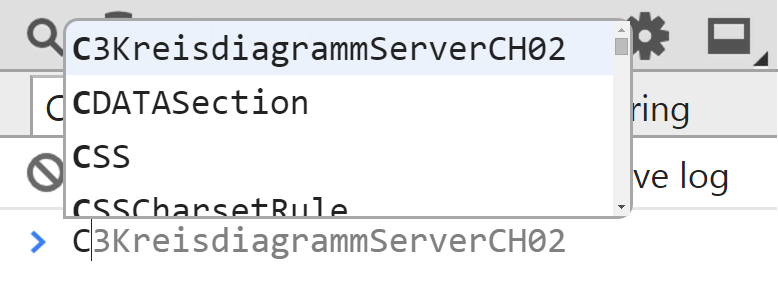
\includegraphics[width=0.50\textwidth]{./img/DevTools/AutoCompl.png}
	\caption[Automatische Vervollständigung der Referenz zum Extension Object]{Automatische Vervollständigung der Referenz zum Extension Object, Quelle: Eigene Abbildung}
	\label{fig:AutoCompl}
\end{figure}


Wenn der Bezeichner des Funktionsobjektes richtig vervollständigt wurde, kann nach Bestätigung der Eingabe das Objekt inspiziert werden. Dies ist in Abbildung \ref{fig:InspectExtensionObject} auf Seite \pageref{fig:InspectExtensionObject} zu sehen.

\begin{figure}[htbp]
	\centering
		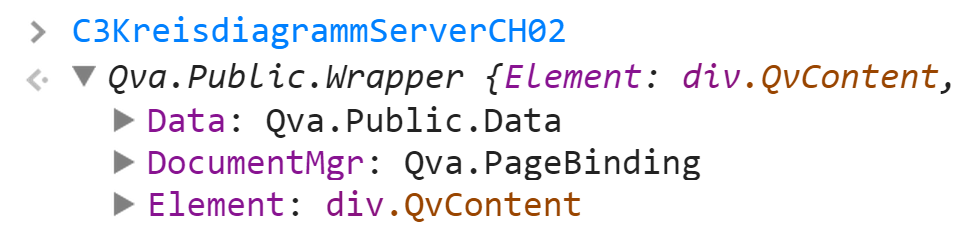
\includegraphics[width=0.60\textwidth]{./img/DevTools/Inspect.png}
	\caption[Inspizierung des Extension Objects in den Chrome DevTools]{Inspizierung des Extension Objects in den Chrome DevTools, \\Quelle: Eigene Abbildung}
	\label{fig:InspectExtensionObject}
\end{figure}


\paragraph{Inspizieren der übermittelten Daten}
\label{lab:InspizierenDerUebermitteltenDaten} 

Ein weiterer Blick in das Funktionsobjekt der Erweiterung mithilfe der Entwicklertools eines Webbrowsers gibt einen Überblick, wie die Daten der Erweiterung strukturiert sind. In der Abbildung \ref{fig:InspectDataRowsAll} sind drei Daten\-sätze zu sehen, die der Erweiterung zur Visualisierung bereitgestellt wurden. Innerhalb des Funktionsobjektes der Erweiterung befinden sich die Daten im Attribut \textit{Data}. Darin ist unter anderem das Attribut \textit{Rows} gespeichert, bei dem es sich um ein Array handelt, in dem jedes Element einen Daten\-satz darstellt. Bei jedem dieser Daten\-sätze handelt es sich wiederum um ein Array, in dem das erste Element die Dimension und das zweite Element den dazugehörigen Wert beschreibt.

\begin{figure}[htbp]
	\centering
		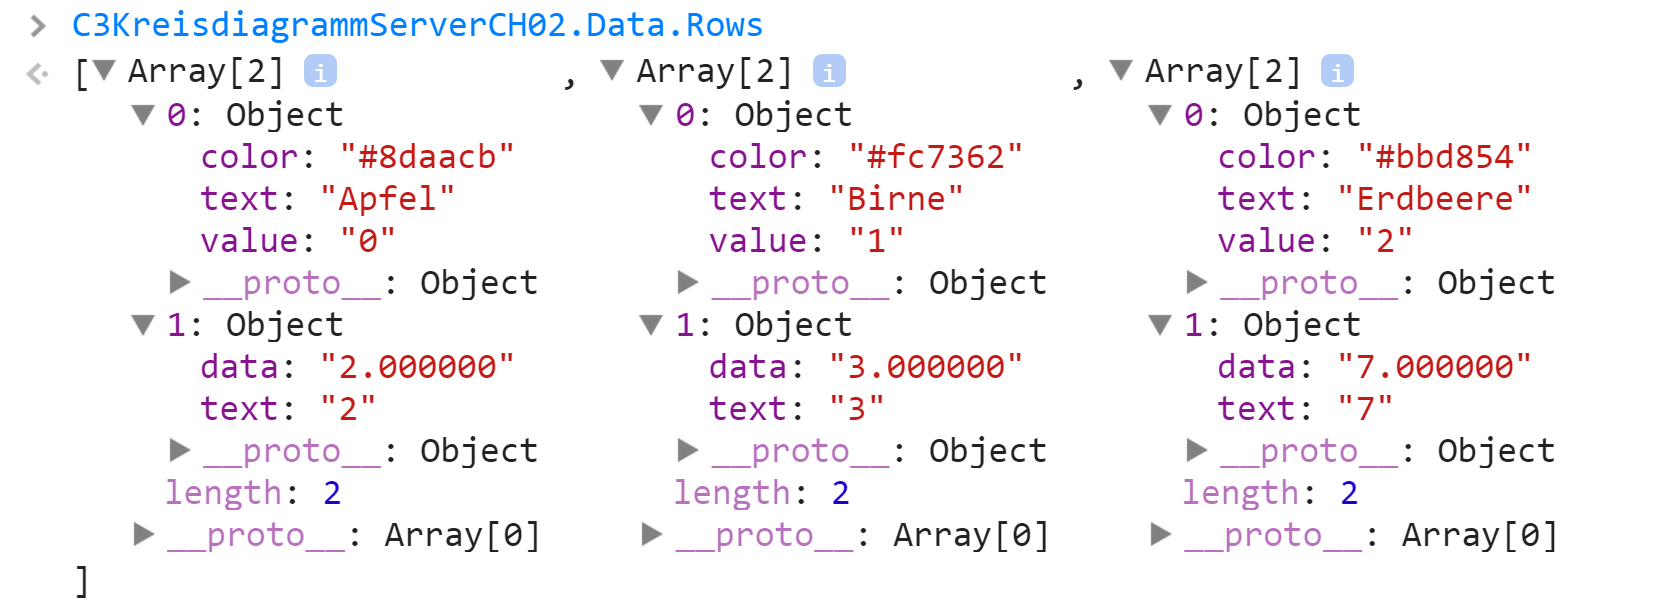
\includegraphics[width=1.00\textwidth]{./img/DevTools/DataRowsAll.png}
	\caption[Inspizierung der Daten des Extension Objects in den Chrome DevTools]{Inspizierung der Daten des Extension Objects in den Chrome DevTools,\\Quelle: Eigene Abbildung}
	\label{fig:InspectDataRowsAll}
\end{figure}

Das Element der Dimension enthält unter anderem das Attribut \textit{text}, welches den anzu\-zeigenden Namen der Dimension repräsentiert, und das Attribut \textit{value}, welches nicht den Wert, aber die Identifikationsnummer des Daten\-satzes speichert. Die Id ist vor allem für die Selektion der Daten wichtig.

Das Element des Wertes enthält die Attribute \textit{data} und \textit{text}, welche beide den gleichen Wert, aber mit einem unterschiedlichen Daten\-typ bereitstellen.


In den Zeilen 16-28 werden die Daten in eine Daten\-struktur überführt, die von der Bibliothek C3.js verstanden wird. In Zeile 16 wird ein Array definiert, dem die Daten\-sätze übergeben werden sollen. In den Zeilen 25 und 26 werden die Daten\-sätze in Form von einem weiteren Array übergeben. C3.js interpretiert das erste Element in diesen Arrays als den Bezeichner und alle weiteren Elemente als Werte, die für das Kreisdiagramm aufsummiert werden würden.\footnote{Vgl. \cite{C3ColumnOrientedData}} Da jedoch lediglich ein Wert als zweites Element hinzugefügt wird, ist eine Summierung nicht nötig.

% XXX Ist das ein Vergleich?


Das Übergeben der Identifikationsnummer als Bezeichner der Spalte ist nötig, da die Selektion der Daten über den Namen nicht ausreicht. Die Namen könnten zur Identifikation des Daten\-satzes übergeben werden. Allerdings wird die Id zur Selektion der Daten benötigt. Für den beim Klick auf den gewünschten Daten\-satz ausgegebenen Namen müsste daher die dazugehörige Id ermittelt werden. Es ist daher mit weniger Implementationsaufwand verbunden, wenn die Id direkt übergeben wird. Die Identifikationsnummern werden jedoch auch in der Legende des Diagramms angezeigt. Stattdessen sollen jedoch die Namen der entsprechenden Dimensionen verwendet werden. Dafür bietet C3.js die Möglich\-keit, für jeden Daten\-satz über die Id einen anzuzeigenden Namen zu deklarieren.\footnote{Vgl. \cite{C3DataName}} Dies geschieht in der Zeile 17, in welcher die Map erstellt wird und in der Zeile 27, in welcher jeder Id der dazugehörige Name der Dimension zugewiesen wird.

% XXX Ist das ein Vergleich?


\paragraph{Auslesen der Parameter}

Alle Parameter, die in der \textit{Definition.xml}-Datei deklariert werden, sind im Funktionsobjekt des Extension Objects im Attribut \textit{Layout} zu finden. In der Abbildung \ref{fig:InspectLayoutParams} wird der Parameter zum Anzeigen der Legende in den Entwicklertools des Chrome Browsers dargestellt.

\begin{figure}[htbp]
	\centering
		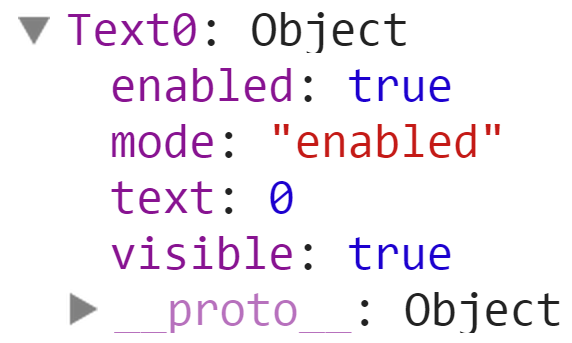
\includegraphics[width=0.25\textwidth]{./img/DevTools/LayoutParams.png}
	\caption[Inspizierung der Parameter des Extension Objects in den Chrome DevTools]{Inspizierung der Parameter des Extension Objects in den Chrome DevTools, Quelle: Eigene Abbildung}
	\label{fig:InspectLayoutParams}
\end{figure}

In der Zeile 29 der \textit{Script.js}-Datei wird der Parameter \textit{Text0} über sein Attribut \textit{text} eingelesen und direkt in einen Wahrheits\-wert konvertiert. Verwendet wird der Wahrheits\-wert in Zeile 47, um das Anzeigen der Legende ein- bzw. auszuschalten.


\paragraph{Vorbereiten der Darstellung}

Jedes Extension Object erhält über das Funktionsobjekt mit der Referenz \textit{Element} Zugriff auf das \textit{div}-Element, in welchem das HTML-Markup gespeichert wird. In Zeile 31 wird dieses \textit{div}-Element zunächst geleert, da sonst Elemente aus dem vorherigen Zeichenvorgang erhalten bleiben würden. In den Zeilen 32-34 wird ein neues \textit{div}-Element mit der CSS-Klasse \textit{kreisdiagramm} erstellt und im Extension Object eingefügt. Es wird bei der Generierung des Diagramms verwendet.
% XXX JQuery wird auch hier genutzt


\paragraph{Generierung des Diagramms}
\label{lab:JsQvGenerierungDesDiagramms} 

Die Zeilen 36-49 zeigen die Generierung des Diagramms. In Zeile 37 wird übermittelt, in welchem Element das Diagramm angezeigt werden soll. Die Daten werden in Zeile 39 übergeben. In Zeile 40 wird festgelegt, dass die Daten als Kreisdiagramm visualisiert werden sollen und in Zeile 44 werden die Ids der Spalten mit den jeweils anzuzeigenden Namen verknüpft.

\paragraph{Selektion der Daten}

In den Zeilen 41-43 wird eine Funktion übergeben, die aufgerufen werden soll, wenn auf einen der Abschnitte des Kreis\-diagramms geklickt wird. In Zeile 42 wird die Funktion \textit{SelectValuesInColumn} der QlikView Ajax API aufgerufen, um eine Selektion der angeklickten Daten vorzunehmen. Der erste Parameter dabei ist die Id der Dimension. Für die Erweiterung wurde ausschließlich eine Dimension deklariert und diese hat die Id 0. Der zweite Parameter erhält die Id des Daten\-satzes, der ausgewählt werden soll. Die Id wurde in der Daten\-struktur von C3 in dem Attribut \textit{id} abgelegt.

Der letzte Parameter trägt den Namen \textit{isFinal}. Die QlikView Ajax Referenz beschreibt den Parameter folgendermaßen:
\begin{quote}
Whether to toggle the selection.\footnote{\cite{JsDocReferenceQvDocumentObjectDataSelectValuesInColumn}}
\end{quote}
Doch diese Erklärung kann für viel Verwirrung sorgen, denn die Funktion des Parameters ist es nicht, die Selektion umzukehren. Tatsächlich legt der Parameter fest, ob die vorige Selektion beibehalten werden soll. Wird als Argument \textit{false} übergeben, ersetzt die neue Selektion die vorige Selektion. Wird \textit{true} übergeben, bleibt die vorige Selektion erhalten und die neue Selektion wird hinzugefügt.

\subsection{Leitfaden zur Erstellung einer QlikView Document Extension mit \\JavaScript}
\label{lab:LeitfadenZurErstellungEinerQlikViewDocumentExtensionMitJavaScript} 

In diesem Kapitel wird die Entwicklung einer Document Extension beschrieben, deren Ziel es ist, das aktuell sichtbare Arbeitsblatt mit dem Drücken der F10-Taste als PNG-Datei herunterzuladen. Sie nutzt die Bibliothek \textit{html2canvas.js}, um die sichtbaren Elemente im Dokument Object Model in ein \textit{canvas}-Element zu zeichnen. Das erstellte Bild soll dann automatisch heruntergeladen werden.

\subsubsection{Erstellen der Dateistruktur}


Die Document Extension wird im Ordner mit dem Namen \textit{DownloadArbeitsblattAlsPng} abgelegt. Die für jede Document Extension benötigten Dateien sind die \textit{Definition.xml}- sowie die \textit{Script.js}-Datei. Darüber hinaus müssen die für die im Folgenden erstellte Document Extension benötigten Bibliotheken in den Ordner heruntergeladen werden. Diese sind \textit{html2canvas.js}\footnote{\url{https://github.com/niklasvh/html2canvas/releases/download/0.4.1/html2canvas.js}}, \textit{canvg.js}\footnote{\url{https://raw.githubusercontent.com/gabelerner/canvg/master/canvg.js}}, \textit{rgbcolor.js}\footnote{\url{https://raw.githubusercontent.com/gabelerner/canvg/master/rgbcolor.js}} und \textit{StackBlur.js}\footnote{\url{https://raw.githubusercontent.com/gabelerner/canvg/master/StackBlur.js}}.










\newpage
\subsubsection{Erstellen eines QlikView-Testdokumentes}

Zum Testen der Document Extension kann das gleiche Dokument zur Anwendung kommen, welches schon im Kapitel \ref{lab:ErstellenEinesQlikViewTestdokumentes} erstellt wurde. Alternativ kann jedoch ein völlig anderes QlikView-Dokument verwendet werden, da die Document Extension nicht von dem Daten\-modell des Dokuments beeinflusst wird. Um die Document Extension zu testen oder bereitzustellen, muss sie dem QlikView-Dokument im Menü über \textit{Einstellungen} > \textit{Eigenschaften des Dokuments…} > \textit{Erweiterungen} hinzugefügt werden. Im Anhang \ref{lab:ScreenshotsVonQlikView} ist dies in den Abbildungen \ref{fig:EigenschaftendesDokumentes} und \ref{fig:DocumentExtensionListe} zu sehen.



\subsubsection{Erstellung der Definition.xml-Datei}

\begin{listing}[htbp]
\begin{minted}[mathescape,
               linenos,
               numbersep=5pt,
               gobble=0,
               frame=lines,
							fontsize=\small,
               framesep=2mm]{xml}
<?xml version="1.0" encoding="utf-8"?>
<ExtensionObject
  Description="Mit F10 das Arbeitsblatt als PNG-Datei herunterladen."
  Type="document">
</ExtensionObject>
\end{minted}
\caption[\textit{Definition.xml}-Datei der DownloadArbeitsblattAlsPng Document Extension]{\textit{Definition.xml}-Datei der DownloadArbeitsblattAlsPng Document Extension, \\Quellcode\textbackslash{}JavaScript\textbackslash{}QlikView\textbackslash{}DownloadArbeitsblattAlsPng\textbackslash{}Definition.xml, \\Quelle: Eigenes Listing}
\label{lst:ArbeitsblattAlsPngDocumentExtensionDefinition}
\end{listing}

Im Listing \ref{lst:ArbeitsblattAlsPngDocumentExtensionDefinition} ist die Definition der Document Extension zu sehen. Ein Label wird nicht angegeben, denn dieses wird in der Liste der verfügbaren Document Extensions nicht angezeigt. Lediglich die Beschreibung kann dort eingesehen werden und wird daher über das Attribut \textit{Description} gesetzt. Anders als bei Extension Objects ist hier das Attribut \textit{Type} mit dem Wert \textit{document} anzugeben, um es als Document Extension zu deklarieren.

\subsubsection{Erstellung der Script.js-Datei}

\begin{listing}[htbp]
\begin{minted}[mathescape,
               linenos,
               numbersep=5pt,
               gobble=0,
               frame=lines,
							fontsize=\small,
               framesep=2mm]{javascript}
var EXTENSION_NAME = "DownloadArbeitsblattAlsPng";
var F10_KEY = 121;

var remoteUrl = Qva.Remote + (Qva.Remote.indexOf('?') >= 0 ? '&' : '?') +
  'public=only&type=document&name=Extensions/' + EXTENSION_NAME;
var jsFiles = [remoteUrl + '/html2canvas.js', remoteUrl + '/rgbcolor.js',
  remoteUrl + '/StackBlur.js', remoteUrl + '/canvg.js'
];
Qv.LoadExtensionScripts(jsFiles, function() {
  Qva.AddDocumentExtension(EXTENSION_NAME, function() {
    $(document).keydown(function(event) {
      if (F10_KEY == event.keyCode) {
        var sheetSize = getSheetSize();
        canvg();
        downloadSheetAsPng(sheetSize);
      }
    });
  });
});

function getSheetSize() {
  var sheetSize = {};
  var elements = document.querySelectorAll('#MainContainer *');
  sheetSize.right = 0;
  sheetSize.bottom = 0;

  for (var i = 0; i < elements.length; i++) {
    var elementRight = elements[i].offsetLeft + elements[i].offsetWidth;
    var elementBottom = elements[i].offsetLeft + elements[i].offsetWidth;
    sheetSize.right = Math.max(sheetSize.right, elementRight);
    sheetSize.bottom = Math.max(sheetSize.bottom, elementBottom);
  }

  return sheetSize;
}

function downloadSheetAsPng(sheetSize) {
  html2canvas(document.body, {
    width: sheetSize.right,
    height: sheetSize.bottom,
    onrendered: function(canvas) {
      var link = document.createElement('a');
      link.href = canvas.toDataURL();
      link.download = 'print.png';
      link.click();
    }
  });
}
\end{minted}
\caption[\textit{Script.js}-Datei der DownloadArbeitsblattAlsPng Document Extension]{\textit{Script.js}-Datei der DownloadArbeitsblattAlsPng Document Extension, \\Quellcode\textbackslash{}JavaScript\textbackslash{}QlikView\textbackslash{}DownloadArbeitsblattAlsPng\textbackslash{}Script.js, \\Quelle: Eigenes Listing}
\label{lst:ArbeitsblattAlsPngDocumentExtensionSkript}
\end{listing}


Das Skript der Document Extension ist im Listing \ref{lst:ArbeitsblattAlsPngDocumentExtensionSkript} auf Seite \pageref{lst:ArbeitsblattAlsPngDocumentExtensionSkript} abgebildet. Einige der Schritte ähneln der Erstellung der \textit{Script.js}-Datei des Extension Objects im Kapitel \ref{lab:ErstellungDerScriptJsDateiQvEoJs}.

Da der Name der Erweiterung mehrmals Verwendung findet, wird er in Zeile 1 einer Variablen zugewiesen. Weiterhin wird in Zeile 2 eine Variable für den Tastencode der F10-Taste gespeichert.

\paragraph{Anfordern von weiteren Dateien}

In den Zeilen 4-9 erfolgt das Nachladen der zusätzlich benötigten JavaScript-Dateien. Beim Zusammensetzen der absoluten Adresse des Ordners, in dem die Erweiterung abgelegt ist, gibt es einen Unterschied zu den Extension Objects. Für Document Extensions muss hier zusätzlich der Parameter \textit{type} mit dem Wert \textit{document} übergeben werden, wie in Zeile 5 zu sehen ist. Die Reihenfolge der in den Zeilen 6 und 7 gelisteten Bibliotheken ist wichtig, da \textit{canvg.js} von \textit{rgbcolor.js} und \textit{StackBlur.js} abhängt und daher nach diesen geladen werden muss.

\paragraph{Funktionsobjekt der Document Extension}


Auch in der Zeile 10 ist ein Unterschied beim Hinzufügen der Erweiterung zu erkennen. Statt \textit{Qva.AddExtension} hat die hier verwendete Methode den Namen \textit{Qva.AddDocumentExtension}. Die beiden Parameter sind jedoch gleich, denn auch hier repräsentiert der erste Parameter den Namen der Erweiterung und der zweite Parameter die dazugehörige Funktion. Diese Funktion wird allerdings im Unterschied zu den Extension Objects nur einmal beim Laden des Dokumentes aufgerufen. 

In der Zeile 11 erfolgt die Deklaration der Funktion, die beim Druck der F10-Taste ausgeführt werden soll. Für solche Events kann, wie in diesem Beispiel zu sehen, \textit{JQuery} verwendet werden. Die Bibliothek wird bereits von der QlikView API importiert und muss daher nicht zusätzlich der Erweiterung hinzugefügt werden.

In Zeile 13 werden die Maße des Bereiches berechnet, indem sich sichtbare Objekte befinden. Die dazugehörige Funktion ist in den Zeilen 21-32 definiert.

Die Bibliothek \textit{html2canvas} arbeitet fehlerhaft beim Zeichnen von SVG-Elementen im Dokument. Das im Kapitel \ref{lab:LeitfadenZurErstellungEinesExtensionObjectsMitJavaScript} erstellte Kreisdiagramm erscheint daher nicht im Bild, da es ebenfalls als SVG-Grafik gezeichnet wird. Mit dem Aufruf der Methode \textit{canvg} in Zeile 14 erfolgt eine Umwandlung aller \textit{svg}-Elemente im Document Object Model in \textit{canvas}-Elemente, die dann korrekt durch \textit{html2canvas} gezeichnet werden. Allerdings ist die Umwandlung ungenau und daher behalten die \textit{svg}-Elemente oft nicht ihre exakte Darstellung, wie in Anhang \ref{lab:BeispielScreenshotDownloadArbeitsblattAlsPng} in Abbildung \ref{fig:ScreenshotSheet} zu sehen ist.

Nach der Umwandlung wird in Zeile 15 die Funktion \textit{downloadSheetAsPng} zum Zeichnen der sichtbaren Elemente aufgerufen. Ihr werden die Maße als erstes Argument übergeben. Die Funktion ist in den Zeilen 37-47 deklariert. Dem ersten Argument der Methode \textit{html2canvas} wird in Zeile 38 das zu zeichnende Element übergeben. Der gesamte Körper des Dokumentes soll gezeichnet werden und daher wird \textit{document.body} übergeben. Beim zweiten Argument handelt es sich um weitere Parameter in Form eines assoziativen Arrays. In den Zeilen 39 und 40 wird der zu zeichnende Bereich auf die bereits berechnete Fläche von sichtbaren Objekten begrenzt. Die Zeilen 41-46 beschreiben die Funktion, die aufgerufen werden soll, wenn das Zeichnen abgeschlossen ist. Die Funktion erstellt ein \textit{a}-Element, welches den Download der im Attribut \textit{href} verwiesenen Datei ermöglicht. Anders als bei herkömmlichen Hyperlinks erhält das Attribut keine Adresse, sondern die Bild\-daten in Form einer Base64-Zeichenkette. Für die Umwandlung sorgt die Funktion \textit{toDataURL} des \textit{canvas}-Objektes. Das Attribut \textit{download} beschreibt den Namen, mit dem das Bild heruntergeladen werden soll. Der Link wird dem Dokument nicht hinzugefügt und ist daher für den Benutzer nicht sichtbar. Dies ist auch nicht nötig, da der Klick auf diesen Link in der Zeile 45 automatisch simuliert wird. Somit startet der Download sofort.

\subsection{Leitfaden zur Erstellung eines Qlik Sense Extension Objects mit \\JavaScript}
\label{lab:LeitfadenZurErstellungEinesQlikSenseExtensionObjectsMitJavaScript} 

Für das im Kapitel \ref{lab:LeitfadenZurErstellungEinesExtensionObjectsMitJavaScript} erstellte Kreisdiagramm wird im Folgenden ein Äquivalent in Qlik Sense erstellt. Im Anhang \ref{lab:ScreenshotsVonQlikSense} in Abbildung \ref{fig:ArbeitsblattQlikSense} ist die Erweiterung in einem Qlik Sense Arbeitsblatt zu sehen.

Für das Beispiel der vorliegenden Arbeit wird die Qlik Sense Workbench verwendet, welche im Kapitel \ref{lab:QlikSenseWorkbench} näher erläutert wurde. Nach dem Klick auf die Schaltfläche \textit{Create New} wird ein Dialog geöffnet. Er ist im Anhang \ref{lab:ScreenshotsVonQlikSense} in Abbildung \ref{fig:WorkbenchCreateNew} dargestellt. Im Eingabefeld \textit{Name} wird \textit{C3Kreisdiagramm} eingetragen. Im Eingabefeld \textit{Template} kann eine beliebige Schablone für die Erweiterung gewählt werden. Für dieses Extension Object wird der Eintrag \textit{Chart template} gewählt. Nach einem Klick auf die Schaltfläche \textit{Create} erscheint das Extension Object unter dem eingegebenen Namen in der Liste der Erweiterungen. Mit einem Klick auf die Erweiterung öffnet sich ein Dialog, in welchem man über die Schaltflächen \textit{Edit} in den Bearbeitungsmodus für die Erweiterung gelangt. Es öffnet sich eine neue Seite mit zwei Reitern für die Dateien \textit{C3Kreisdiagramm.qext} und \textit{C3Kreisdiagramm.js}.

\subsubsection{C3Kreisdiagramm.qext}


An der Datei \textit{C3Kreisdiagramm.qext} sollten einige Änderungen durchgeführt werden. Das Attribut \textit{icon} erhält statt dem Wert \textit{bar-chart-vertical} den Wert \textit{pie-chart,} damit die Erweiterung in der Liste der verfügbaren Erweiterungen mit einem Kreisdiagramm als Vorschaubild erscheint. Alternativ kann für das Attribut \textit{preview} der Name einer Bild\-datei angegeben werden. Für diese Erweiterung wird das Attribut entfernt. Außerdem erhält das Attribut \textit{author} den Namen des Verfassers dieser Arbeit. Das Listing \ref{lst:QlikSenseC3KreisdiagrammC3Kreisdiagrammqext} zeigt die durchgeführten Änderungen an der Datei.

\begin{listing}[htbp]
\begin{minted}[mathescape,
               linenos,
               numbersep=5pt,
							fontsize=\small,
               gobble=0,
               frame=lines,
               framesep=2mm]{javascript}
{
  "name": "C3Kreisdiagramm",
  "description": "${name}",
  "icon": "pie-chart",
  "type": "visualization",
  "version": 1,
  "author": "Alexander Johr"
}
\end{minted}
\caption[\textit{.qext}-Datei des Qlik Sense C3Kreisdiagramm Extension Objects]{\textit{.qext}-Datei des Qlik Sense C3Kreisdiagramm Extension Objects, \\Quellcode\textbackslash{}JavaScript\textbackslash{}Qlik Sense\textbackslash{}C3Kreisdiagramm\textbackslash{}C3Kreisdiagramm.qext, \\Quelle: Eigenes Listing}
\label{lst:QlikSenseC3KreisdiagrammC3Kreisdiagrammqext}
\end{listing}

\subsubsection{Weitere Module erstellen}
\label{lab:QlikSenseWeitereModuleErstellen} 

Da Qlik Sense die Bibliothek RequireJS verwendet, ist es sehr einfach möglich, die Definition und die initialen Eigenschaften der Erweiterung in externe JavaScript-Dateien auszulagern. Dies ist in Vorbereitung auf die Portierung der Erweiterung nach Dart sehr nützlich, da die JavaScript-Dateien nicht verändert werden müssen. Es handelt sich bei den Parametern lediglich um assoziative Arrays, bei denen es keinen Vorteil hat, sie in die Dart-Syntax zu überführen. Vielmehr erfordert es einen zusätzlichen Aufwand, wie in Anhang \ref{lab:initialPropertiesQlikSenseExtensionObjectDartSyntax} im Listing \ref{lst:initialPropertiesQlikSenseExtensionObjectDartSyntax} zu sehen ist. Außerdem wird der Erweiterung ein CSS-Stylesheet hinzugefügt. Dieser kann ebenso durch RequireJS eingebunden werden.


Über die Schaltfläche \textit{New File} können weitere Dateien hinzugefügt werden. In dem Eingabefeld \textit{Name} wird daher zunächst \textit{initialProperties.js} anschließend \textit{definition.js} und schließlich \textit{style.css} eingegeben und jeweils mit der Schaltfläche \textit{Create} bestätigt. Im Folgenden wird in beiden JavaScript-Dateien jeweils mit dem Befehl \textit{define} die Definition des Moduls eingeleitet. Bei der CSS-Datei ist dies nicht nötig, da diese nur als Text eingelesen wird.

\paragraph{CSS-Stylesheet}

Wie schon bereits im Kapitel \ref{lab:HinzufügenEinesCSSStylesheet} für das QlikView Extension Object beschrieben, bedarf es einer CSS-Anweisung für die Erweiterung. Sie sorgt dafür, dass die generierte Vektorgrafik korrekt im zu zeichnenden Bereich erstellt wird. Der Inhalt, der im Reiter \textit{style.css} eingetragen wird, ist im Listing \ref{lst:QlikSenseC3KreisdiagrammStyleCss} zu sehen.

\begin{listing}[htbp]
\begin{minted}[mathescape,
               linenos,
               numbersep=5pt,
							fontsize=\small,
               gobble=0,
               frame=lines,
               framesep=2mm]{css}
.kreisdiagramm { height: 100%; width: 100%; }
\end{minted}
\caption[\textit{style.css}-Datei des Qlik Sense C3Kreisdiagramm Extension Objects]{\textit{style.css}-Datei des Qlik Sense C3Kreisdiagramm Extension Objects, \\Quellcode\textbackslash{}JavaScript\textbackslash{}Qlik Sense\textbackslash{}C3Kreisdiagramm\textbackslash{}style.css, \\Quelle: Eigenes Listing}
\label{lst:QlikSenseC3KreisdiagrammStyleCss}
\end{listing}

\paragraph{Initiale Eigenschaften}

Im Listing \ref{lst:QlikSenseC3KreisdiagrammInitialPropertiesJs} werden die initialen Eigenschaften des Extension Objects deklariert. Hier können beispielsweise Standardwerte für die Dimensionen - in Zeile 4 - und für die Formeln - in Zeile 5 - festgelegt werden. Durch den Befehl \textit{define} in Zeile 1 wird das assoziative Array unter dem Namen der JavaScript-Datei definiert. Es gibt keine Abhängig\-keiten von anderen Modulen, daher erhält die Funktion nur einen Parameter, nämlich die aufzurufende Funktion des Moduls. Sie gibt das Array zurück.

\begin{listing}[htbp]
\begin{minted}[mathescape,
               linenos,
               numbersep=5pt,
							fontsize=\small,
               gobble=0,
               frame=lines,
               framesep=2mm]{javascript}
define(function() {
  return {
    version: 1.0,
    qHyperCubeDef: {
      qDimensions: [],
      qMeasures: [],
      qInitialDataFetch: [{
        qWidth: 10, qHeight: 50
      }]
    }
  };
});
\end{minted}
\caption[\textit{initialProperties.js}-Datei des Qlik Sense C3Kreisdiagramm Extension Objects]{\textit{initialProperties.js}-Datei des Qlik Sense C3Kreisdiagramm Extension Objects, \\Quellcode\textbackslash{}JavaScript\textbackslash{}Qlik Sense\textbackslash{}C3Kreisdiagramm\textbackslash{}initialProperties.js, \\Quelle: Eigenes Listing}
\label{lst:QlikSenseC3KreisdiagrammInitialPropertiesJs}
\end{listing}

\paragraph{Definition der Dimensionen, Formeln, Parameter und Eingabefelder}

Eine Datei zum Beschreiben des Konfigurationsdialoges, wie es sie unter dem Namen \textit{Properties.qvpp} in QlikView gab - siehe Kapitel \ref{lab:PropertiesQvpp} -, existiert in Qlik Sense nicht. Das Aussehen des Dialoges ist bereits festgelegt und lediglich die gewünschten Eingabefelder müssen angegeben werden.

Listing \ref{lst:QlikSenseC3KreisdiagrammDefinitionJs} zeigt die Definition des Extension Objects. Die Hauptnavigation ist eine Liste von Menüpunkten - deklariert in Zeile 3 - die in einem \textit{accordion} - zugewiesen in Zeile 4 - dargestellt werden. In einigen Einträgen ist die Zuweisung des Attributes \textit{uses} angegeben. Damit wird die Standardkonfiguration geladen. Alle weiteren Eigenschaften konfigurieren diese Standardeinstellungen.

\begin{listing}[htbp]
\begin{minted}[mathescape,
               linenos,
               numbersep=5pt,
							fontsize=\small,
               gobble=0,
               frame=lines,
               framesep=2mm]{javascript}
define(function() {
  return {
    type: "items",
    component: "accordion",
    items: {
      dimensions: {
        uses: "dimensions",
        min: 1, max: 1
      },
      measures: {
        uses: "measures",
        min: 1, max: 1
      },
      sorting: {
        uses: "sorting"
      },
      settings: {
        uses: "settings",
        items: {
          legend: {
            type: "boolean",
            defaultValue: true,
            label: "Zeige Legende",
            ref: "showLegend"            
          },
        },
      }
    }
  };
});
\end{minted}
\caption[\textit{definition.js}-Datei des Qlik Sense C3Kreisdiagramm Extension Objects]{\textit{definition.js}-Datei des Qlik Sense C3Kreisdiagramm Extension Objects, \\Quellcode\textbackslash{}JavaScript\textbackslash{}Qlik Sense\textbackslash{}C3Kreisdiagramm\textbackslash{}definition.js, \\Quelle: Eigenes Listing}
\label{lst:QlikSenseC3KreisdiagrammDefinitionJs}
\end{listing}

Es sollen genau eine Dimension und eine Formel für das Extension Object existieren. Daher werden das Minimum und das Maximum für die Dimensionen - in Zeile 8 - und für die Formeln - in Zeile 12 - auf \textit{1} gesetzt. Neben der Standardkonfiguration soll eine komplett neue Eigenschaft hinzugefügt werden, nämlich der Wahrheits\-wert zum Anzeigen der Legende. Diese soll in der Rubrik der Einstellungen erscheinen und wird daher dem Eintrag \textit{settings} in den Zeilen 17-27 hinzugefügt. Durch den Eintrag \textit{items} kann eine weitere Unternavigation hinzugefügt werden. In dieser ist nur das Eingabefeld \textit{Legend} präsent. In den Zeilen 21 und 23 wird festgelegt, dass es sich um einen Wahrheits\-wert handelt, der standardmäßig den Wert \textit{wahr} hat und der anzuzeigende Text \textit{Zeige Legende} lauten soll. In Zeile 24 wird ein Bezeichner dem Attribut \textit{ref} zugewiesen, unter welchem die Eingabe des Feldes im Skript zu finden sein wird.



\subsubsection{Herunterladen der Bibliotheken}
\label{lab:HerunterladenDerBibliothekenQlikSense} 

Wie bereits für das Extension Object C3Kreisdiagramm für QlikView müssen ebenfalls die Dateien der Bibliotheken D3 und C3 in den Ordner der erstellten Erweiterung heruntergeladen werden. Anders als im Kapitel \ref{lab:QlikViewQvExtAnfordernVonWeiterenDateien} wird diesmal nicht die verkleinerte \textit{c3.min.js}-Datei, sondern die vollständige \textit{c3.js}-Datei verwendet. Der Grund dafür ist, dass diese Datei für das Funktionieren mit RequireJS modifiziert werden muss.
Die im Folgenden notwendigen Dateien sind also: \textit{d3.min.js} \footnote{\url{https://github.com/mbostock/d3/blob/master/d3.min.js}}, \textit{c3.js} \footnote{\url{https://github.com/masayuki0812/c3/blob/master/c3.js}} und \textit{c3.min.css} \footnote{\url{https://github.com/masayuki0812/c3/blob/master/c3.min.css}}.

\paragraph{Modifizieren der c3.js-Datei }

Die Definition der Module erfolgt durch RequireJS nicht nur über den Dateinamen, sondern auch über den Dateipfad.\footnote{Vgl. \cite{RequireJSAPILoadJavaScriptFiles}} So wird beispielsweise die Datei \textit{C3Kreisdiagramm.js} mit dem Pfad \textit{extensions/C3Kreisdiagramm/C3Kreisdiagramm} erstellt. Die \textit{d3.min.js}-Datei befindet sich in demselben Ordner und wird daher auch relativ zu diesem Pfad definiert, und zwar unter \textit{extensions/C3Kreisdiagramm/d3.min}. Dies ist jedoch problematisch, da die Bibliothek C3 die Abhängig\-keit D3 im Pfad \textit{d3} erwartet. Dies ist im Listing \ref{lst:RequireJsBefehlDefineC3Js} in der Zeile 6902 zu sehen.

\begin{listing}[htbp]
\begin{minted}[mathescape,
               linenos,
               numbersep=5pt,
							firstnumber=6901,
							fontsize=\small,
               gobble=0,
               frame=lines,
               framesep=2mm]{javascript}
if (typeof define === 'function' && define.amd) {
  define("c3", ["d3"], c3);
} else if ('undefined' !== typeof exports && 'undefined' !== typeof module) {
  module.exports = c3;
} else {
  window.c3 = c3;
}
\end{minted}
\caption[RequireJS-Befehl \textit{define} in der C3.js-Bibliothek]{RequireJS-Befehl \textit{define} in der C3.js-Bibliothek der Version 0.4.9, c3.js, \\Quelle: \cite{c3masayuki0812c3}}
\label{lst:RequireJsBefehlDefineC3Js}
\end{listing}

Unter dem Pfad \textit{d3} ist die Abhängig\-keit nicht zu finden, was dazu führt, dass C3 nicht initialisiert werden kann und die Referenz auf die Bibliothek im Skript \textit{null} sein wird. Dies wird bei der Generation des Diagramms zu einem Fehler führen. Daher ist es nötig den Ausdruck zu modifizieren, indem der tatsächliche Pfad der Bibliotheken angegeben wird. Im Listing \ref{lst:KorrekturDesDefineBefehlsInC3FuerJavaScript} auf Seite \pageref{lst:KorrekturDesDefineBefehlsInC3FuerJavaScript} ist die modifizierte Zeile 6902 einsehbar.
% XXXX Abbildung einfügen

\begin{listing}[htbp]
\begin{minted}[mathescape,
               linenos,
               numbersep=5pt,
							firstnumber=6901,
               gobble=0,
							fontsize=\small,
               frame=lines,
               framesep=2mm]{javascript}
if (typeof define === 'function' && define.amd) {
  define("extensions/C3Kreisdiagramm/c3", ["extensions/C3Kreisdiagramm/d3.min"]
    , c3);
} else if ('undefined' !== typeof exports && 'undefined' !== typeof module) {
  module.exports = c3;
} else {
  window.c3 = c3;
}
\end{minted}
\caption[Korrektur des \textit{define}-Befehls in der C3.js-Bibliothek]{Korrektur des \textit{define}-Befehls in der C3.js-Bibliothek, \\Quellcode\textbackslash{}JavaScript\textbackslash{}Qlik Sense\textbackslash{}C3Kreisdiagramm\textbackslash{}c3.js, \\Quelle: \cite{c3masayuki0812c3} modifiziert durch Verf.}
\label{lst:KorrekturDesDefineBefehlsInC3FuerJavaScript}
\end{listing}

\newpage
\paragraph{Anpassen der wbfolder.wbl-Datei}

Damit die soeben hinzugefügten Dateien auch in der Qlik Sense Workbench als Reiter auftauchen, müssen sie in der \textit{wbfolder.wbl}-Datei gelistet werden. Im Listing \ref{lst:QlikSenseC3KreisdiagrammWbfolderWblDatei} ist die \textit{wbfolder.wbl}-Datei nach dem Hinzufügen der betroffenen Dateien zu sehen.

\begin{listing}[htbp]
\begin{minted}[mathescape,
               linenos,
               numbersep=5pt,
							fontsize=\small,
               gobble=0,
               frame=lines,
               framesep=2mm]{javascript}
C3Kreisdiagramm3.qext;
C3Kreisdiagramm3.js;
initialProperties.js;
definition.js;
style.css;
d3.min.js;
c3.min.css;
c3.js;
\end{minted}
\caption[\textit{wbfolder.wbl}-Datei des Qlik Sense C3Kreisdiagramm Extension Objects ]{\textit{wbfolder.wbl}-Datei des Qlik Sense C3Kreisdiagramm Extension Objects, \\Quellcode\textbackslash{}JavaScript\textbackslash{}Qlik Sense\textbackslash{}C3Kreisdiagramm\textbackslash{}wbfolder.wbl, \\Quelle: Eigenes Listing}
\label{lst:QlikSenseC3KreisdiagrammWbfolderWblDatei}
\end{listing}

\subsubsection{C3Kreisdiagramm.js}
\label{lab:C3KreisdiagrammJs} 

Im Listing \ref{lst:QlikSenseC3KreisdiagrammC3KreisdiagrammJs} auf Seite \pageref{lst:QlikSenseC3KreisdiagrammC3KreisdiagrammJs} ist der Haupteinstiegspunkt des Extension Objects zu sehen. In den Zeilen 1 und 2 werden die erstellten Module für die Definition und die initialen Eigenschaften sowie die benötigten Bibliotheken als Abhängig\-keiten dieses Moduls definiert. Der zweite Parameter in der Zeile 3 ist eine Funktion, welche die angegebenen Abhängig\-keiten als Parameter erhält. Aus diesem Grund ist die Anzahl der Parameter gleich der Anzahl der Einträge der Liste von Abhängig\-keiten. Weiterhin ist auch die Reihenfolge gleich, sodass der erste Eintrag der Abhängig\-keiten auch dem ersten Parameter der Funktion zugewiesen wird.

\begin{listing}[htbp]
\begin{minted}[mathescape,
               linenos,
               numbersep=5pt,
							fontsize=\small,
               gobble=0,
               frame=lines,
               framesep=2mm]{javascript}
define(["./initialProperties", "./definition", "./c3",
  "text!./c3.min.css", "text!./style.css"], 
  function(initialPropertiesJs, definitionJs, c3Js, c3Css, styleCss) {
  'use strict';

  $("<style>").html(c3Css).appendTo("head");
  $("<style>").html(styleCss).appendTo("head");

  return {
    initialProperties: initialPropertiesJs,
    definition: definitionJs,
    paint: function($contentDiv, extensionData) {
      var extensionObject = this;
      var objectId = extensionData.qInfo.qId;
      window["C3KreisdiagrammObject" + objectId] = extensionObject;
      window["C3KreisdiagrammData" + objectId] = extensionData;

      var c3Columns = new Array();
      var idNameMap = {};
      extensionObject.backendApi.eachDataRow(function(rownum, row) {
        var id = row[0].qElemNumber;
        var dimension = row[0].qText;
        var value = row[1].qText;
        var c3Column = [id, value];
        c3Columns.push(c3Column);
        idNameMap[id] = dimension;
      });

      $contentDiv.empty();
      var chartDivElement = $("<div>");
      chartDivElement.className = "kreisdiagramm";
      $contentDiv.append(chartDivElement);

      c3Js.generate({
        bindto: $contentDiv[0],
        data: {
          columns: c3Columns,
          type: 'pie',
          onclick: function(data) {
            extensionObject.backendApi.selectValues(0, [parseInt(
              data.id)], false);
          },
          names: idNameMap
        },
        legend: { show: extensionData.showLegend }
      });
    }
  };
});
\end{minted}
\caption[\textit{.js}-Datei des Qlik Sense C3Kreisdiagramm Extension Objects ]{\textit{.js}-Datei des Qlik Sense C3Kreisdiagramm Extension Objects, \\Quellcode\textbackslash{}JavaScript\textbackslash{}Qlik Sense\textbackslash{}C3Kreisdiagramm\textbackslash{}C3Kreisdiagramm.js, \\Quelle: Eigenes Listing}
\label{lst:QlikSenseC3KreisdiagrammC3KreisdiagrammJs}
\end{listing}


Bei den beiden letzten Abhängig\-keiten \textit{text!./c3.min.css} und \textit{text!./style.css} handelt es sich um CSS-Dateien, welche nicht als JavaScript-Objekte eingelesen werden können und daher als Text interpretiert werden müssen. Aufgrund dessen beginnen beide Abhängig\-keiten mit dem Ausdruck \textit{text!}, welcher angibt, dass der Inhalt der Datei als Zeichenkette dem Parameter übergeben werden soll.\footnote{Vgl. \cite{SpecifyATextFileDependency}}

In den Zeilen 6 und 7 werden die Inhalte dieser CSS-Dateien über die Parameter \textit{c3Css} und \textit{styleCss} im \textit{head}-Element des Dokuments als \textit{style}-Elemente eingefügt. Auffällig an den beiden Codezeilen ist die Ähnlich\-keit der Syntax mit JQuery. Qlik Sense bindet diese Bibliothek nicht ein, dennoch sind JQuery-Befehle verfügbar, da Qlik Sense das AngluarJS-Framework verwendet.
\begin{quote}
AngularJS [...] builds on the core functionality of jQuery. In fact, AngularJS contains a cut-down version of jQuery called jqLite [...].\footnote{\cite[S. 47]{Freeman2014}}
\end{quote}


Beginnend ab der Zeile 9 wird das assoziative Array des in dieser Datei definierten Moduls zurückgegeben. In den Zeilen 10 und 11 können nun die in den vorherigen beiden Schritten erstellten Module für das \textit{initialProperties}- und das \textit{definition}-Attribut übergeben werden.

Das letzte wichtige Attribut für das Extension Object ist \textit{paint}, welches die Funktion erhält, die für das Zeichnen verwendet werden soll. Sie wird beispielsweise bei der Erstellung oder Manipulation der Instanz der Erweiterung und bei der Selektion von Daten aufgerufen. 

Die Funktion erhält zwei Parameter. Der erste Parameter enthält das \textit{div}-Element, welches dem Extension Object zum Zeichnen zur Verfügung gestellt wird. Über diese Referenz können JQuery-Funktionen aufgerufen werden. Daher wurde dem Namen der Referenz ein Dollarzeichen vorangestellt, um zu verdeutlichen, dass es sich um eine JQuery-Referenz und nicht um eine herkömmliche Referenz auf ein \textit{div}-Element handelt. Dem zweiten Parameter werden die aktuellen Daten und die aktuelle Selektion, sowie weitere Informationen zum Extension Object übergeben. 

Darüber hinaus gibt es jedoch noch weitere Informationen des Extension Objects, welche über die Referenz \textit{this} im Kontext der Funktion verfügbar sind. Damit die Referenz nicht von einem weiteren Funktionskörper überschrieben wird, erfolgt eine Zuweisung von \textit{this} zur lokalen Variable \textit{extensionObject} in Zeile 13.

Das Attribut \textit{extensionData.qInfo.qId} wird in Zeile 14 ausgelesen, um sie einer lokalen Variable \textit{objectId} zuzuweisen. Sie wird in den Zeilen 15 und 16 verwendet, um die Information zum Objekt sowie die Information zu den aktuellen Daten und Selektionen im globalen Kontext \textit{window} zu speichern. Auf diese Weise ist es möglich, im Browser durch Inspektion der Objekte Hinweise für das weitere Vorgehen zu erhalten.

\paragraph{Inspektion der Daten}


Nachdem die Erweiterung installiert und einer Anwendung hinzu\-gefügt wurde, ist es möglich, in den Entwicklungswerkzeugen des Browsers weitere Informationen über die globalen Variablen zu erhalten. Für dieses Beispiel wird dem Extension Object die Dimension \textit{Produkt} und die Formel \textit{Menge} hinzugefügt.
% XXX erstellung einer Anwendung woanders erläutern

Durch Eintippen der Zeichenkette \textit{C3KreisdiagrammData} in der JavaScript-Konsole wird das konkrete Objekt vorgeschlagen. Dies ist ratsam, da die Id, die für die Referenz verwendet wird, variabel ist. Das Objekt enthält unter anderem das Attribut \textit{qHyperCube.qDataPages}, in welchem die aktuellen Daten einsehbar sind. Dies ist in Abbildung \ref{fig:qDataPages} auf Seite \pageref{fig:qDataPages} zu sehen.

Die Daten sind ähnlich aufgebaut wie in QlikView, was im Kapitel \ref{lab:InspizierenDerUebermitteltenDaten} nachgeschlagen werden kann. Jeder Daten\-satz ist ein Array mit zwei Elementen.
Im ersten Element ist unter anderem die Id, welche zur Selektion des Daten\-satzes notwendig ist, im Attribut \textit{qElemNumber} gespeichert. Weiterhin ist die Bezeichnung der Dimension im Attribut \textit{qText} zu finden. 

\begin{figure}
	\centering
		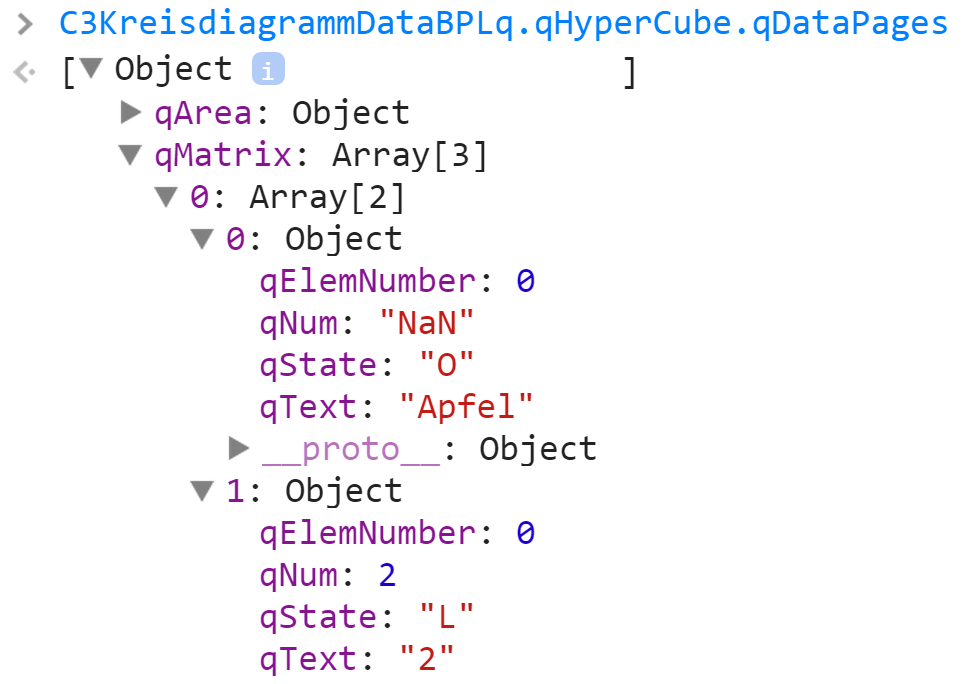
\includegraphics[width=0.60\textwidth]{img/QsDevTools/qDataPages.PNG}
	\caption[Daten des Qlik Sense Extension Object C3Kreisdiagramm]{Daten des Qlik Sense Extension Object C3Kreisdiagramm, \\Quelle: Eigene Abbildung}
	\label{fig:qDataPages}
\end{figure}

Im zweiten Element des Arrays ist der Wert des Daten\-satzes in unterschiedlichen Daten\-formaten vorhanden. Das Attribut \textit{qText} speichert den Wert als Zeichenkette während \textit{qNum} den Wert als Zahl beinhaltet.

\paragraph{Auslesen der Daten}

In den Zeilen 18-28 des Listings \ref{lst:QlikSenseC3KreisdiagrammC3KreisdiagrammJs} auf Seite \pageref{lst:QlikSenseC3KreisdiagrammC3KreisdiagrammJs} wird das Auslesen der Daten vorgenommen. Wie bereits für das Kreisdiagramm Extension Object unter QlikView werden auch hier die Daten in ein Format überführt, die von der C3-Bibliothek verwendet werden können. Ebenso erfolgt wiederum eine Zuweisung des Dimensionsnamens, zu der dazugehörigen Id. Dies kann im Kapitel \ref{lab:InspizierenDerUebermitteltenDaten} nachgelesen werden. Für Qlik Sense unterscheiden sich hier lediglich der Zugriff auf die Daten mittels einer Funktion statt einer Schleife und die Bezeichner der Attribute.

In Qlik Sense kann über die Funktion \textit{eachDataRow} des Attributes \textit{backendApi} des Funktions\-objektes \textit{extensionObject} auf die Daten zugegriffen werden.\footnote{Vgl. \cite{eachDataRowMethod}} Ihr wird eine Funktion übergeben, welcher im ersten Parameter die Zeilen\-nummer des Daten\-satzes und im zweiten Parameter der Daten\-satz selbst übergeben wird. In den Zeilen 21-23 werden die Attribute dieses Daten\-satzes ausgelesen. Die Zeilennummer findet hier keine Anwendung.

\paragraph{Zeichnen des Diagramms}

In den Zeilen 29-32 wird das \textit{div}-Element zunächst geleert und ihm anschließend ein weiteres \textit{div}-Element mit der CSS-Klasse \textit{kreisdiagramm} hinzugefügt.
In den Zeilen 34-46 erfolgt die Generierung des Diagramms. Wie schon im Kapitel \ref{lab:JsQvGenerierungDesDiagramms} beschrieben, werden auch hier die Daten, der Diagrammtyp und die Dimensionsnamen über\-geben. 

Die Unterschiede zum Vorgehen in QlikView sind die folgenden:

Da es sich bei dem \textit{\$contentDiv} nicht um eine herkömmliche Referenz auf ein \textit{div}-Element handelt, sondern um eine Referenz auf ein JQuery-Objekt, welches das \textit{div}-Element referenziert, ist die direkte Zuweisung der Referenz nicht möglich. Bei dem Objekt handelt es sich um eine Liste, welche genau ein Element enthält, nämlich die Referenz auf das tatsächliche \textit{div}-Element. Daher wird dem Attribut \textit{bindto} dieses erste Element mit dem Ausdruck \textit{\$contentDiv[0]} übergeben. Die Selektion der Daten wird in Qlik Sense mit der Methode \textit{selectValues} des Attributes \textit{backendApi} des Funktionsobjektes \textit{extensionObject} umgesetzt. 

Die Parameter sind weitestgehend die gleichen geblieben. Der erste Parameter ist die Id der Dimension. Der zweite Parameter ist diesmal eine Liste an auszuwählenden Ids. Da nur eine Id ausgewählt werden soll, enthält die Liste nur ein Element. In QlikView war es möglich, ausschließlich eine Id anzugeben. Sollten mehrere Ids ausgewählt werden, so bedarf es in QlikView der Übergabe einer einzelnen Zeichenkette, welche die Ids durch Kommata getrennt enthält. In Qlik Sense ist dagegen nur noch die Auswahl über eine Liste von Ids möglich. Der letzte Parameter gibt den Selektionsmodus an. Ist der Wert wahr, wird die neue Selektion der vorherigen Selektion hinzugefügt. Ist der Wert unwahr, so ersetzt die neue Selektion die vorherige.\footnote{Vgl. \cite{JsDocReferenceQvDocumentObjectDataSelectValuesInColumn}}



\section{Entwicklung von Erweiterungen mit Dart}
\label{lab:EntwicklungVonErweiterungenMitDart} 

Dieses Kapitel beschäftigt sich mit der Entwicklung von Extension Objects und Document Extensions für QlikView und Qlik Sense mithilfe der Programmiersprache Dart. Zu diesem Zweck wird jedoch zunächst eine Klassen\-bibliothek entwickelt, mit der die QlikView Ajax API sowie die Qlik Sense Extensions API abstrahiert werden soll. Die für die Entwicklung von Erweiterungen essenziellen Funktionen der jeweiligen Implementationen sollen in der Klassen\-bibliothek über dieselben Schnittstellen erreichbar sein. Anschließend erfolgt die Implementierung zweier sogenannter Pub Transformer zur automatisierten Bereitstellung der Erweiterungen auf den jeweiligen Servern. Abschließend werden die Erweiterungen, die in dem Kapitel \ref{lab:VorbereitendeEntwicklungVonErweiterungenMitJavaScript} entwickelt wurden, in die Dart Programmiersprache portiert.

\subsection{Entwicklung einer Klassenbibliothek zur Verallgemeinerung der \\QlikView und Qlik Sense API}
\label{lab:EntwicklungKlassenbibliothekVerallgemeinerungQlikViewQlikSenseAPI} 

Die QlikView Ajax API sowie die Qlik Sense Extensions API lassen kaum Gemeinsam\-keiten erkennen. Die Objekte, deren Attribute und Funktionen haben unterschiedliche Namen. Auch die Parameter unterscheiden sich teilweise in ihrem Daten\-typ. Im weiteren Verlauf dieses Kapitels werden einige dieser Funktionen vorgestellt und ihre Unterschiede erläutert.

Die enorme Ungleich\-heit hat zwei Nachteile zur Folge. Hat man bereits den Umgang mit einer API kennengelernt, hilft dies nur sehr wenig, um sich in die andere einzuarbeiten. Weiterhin ist das Portieren einer Erweiterung zwischen den beiden Plattformen sehr schwierig, da fast jede Anweisung ausgetauscht werden muss.

Darüber hinaus weist die QlikView Ajax API einige Inkonsistenzen und fehlleitende Bezeichner für Funktionen und Parameter auf. So gibt es beispielsweise die Methode \textit{GetCurrentSelections}. Statt der aktuellen Selektion gibt die Methode \textit{undefined} zurück. Ungleich einer gewöhnlichen Getter-Funktion muss ihr ein Objekt im ersten Parameter übergeben werden. Das Objekt sollte ein Attribut \textit{onChange} haben, bei dem es sich um eine Callback-Funktion handelt. Die Funktion wird immer dann aufgerufen, wenn sich an der aktuellen Selektion etwas ändert.\footnote{Vgl. \cite{JsDocReferenceGetCurrentSelections}} Es handelt sich daher also nicht um eine Getter-Funktion, obwohl ihr Name dies vermuten lässt. 

Ein weiteres Beispiel dafür, dass die QlikView Ajax API sich nur sehr schwer bedienen lässt, ist im Anhang \ref{lab:FehlerhafteVerwendungDerQlikViewAjaxAPI} zu sehen.

Aufgrund der Ungleich\-heit beider APIs sowie der erschwerten Anwendung wurde für diese Arbeit eine Klassen\-bibliothek erstellt, die die Entwicklung von Erweiterungen stark ver\-einfachen soll. Ein Klassendiagramm der Klassenbibliothek ist im Anhang \ref{lab:KlassendiagrammDerKlassenbibliothek} in Abbildung \ref{fig:Klassendiagramm} zu sehen.


\subsubsection{Erstellen des Projektes}

Das Projekt wird als sogenanntes Pub Package erstellt. Der Dart Editor kann dabei sehr hilfreich sein, da es für diese Art von Projekt eine Vorlage mit dem Namen \textit{package} gibt. Das Projekt erhält den Namen qlikview\_qlik\_sense\_extensions. Für die Programmiersprache Dart existiert ein Styleguide, der empfiehlt, Bibliotheken und Dateinamen mit Kleinbuchstaben und Unterstrichen zu benennen.\footnote{Vgl. \cite{DartStyleGuide}}


Das Pub Package enthält unter anderem den Ordner \textit{lib}. Es handelt sich um den Ordner, in dem die Quelldateien abgelegt werden sollen, die von anderen Projekten verwendet werden. Andere Ordner, wie beispielsweise die Ordner \textit{test} und \textit{example}, können ebenfalls Dart-Quelldateien enthalten, welche jedoch nicht in andere Projekte eingebunden werden.\footnote{Vgl. \cite{PubPackageLayoutConventions}}
 
Ein Dartprojekt enthält im Wurzelordner eine \textit{pubspec.yaml}-Datei. Dabei handelt es sich sozusagen um die Projektdatei, in welcher grundlegende Informationen zum Projekt gespeichert werden. Sie enthält auch eine Liste aller Abhängig\-keiten des Projektes, die automatisch heruntergeladen werden können. Darüber hinaus gibt es die Möglich\-keit, sogenannte Pub Transformer anzugeben, die bei jedem Bildprozess aufgerufen werden.\footnote{Vgl. \cite{PubspecFormat}} Im Listing \ref{lst:QlikviewQlikSenseExtensionsPubspecYaml} ist die \textit{pubspec.yaml}-Datei des soeben erstellten Projektes mit den nötigen Änderungen zu sehen.



\begin{listing}[htbp]
\begin{minted}[mathescape,
               linenos,
               numbersep=5pt,
							fontsize=\small,
               gobble=0,
               frame=lines,
               framesep=2mm]{yaml}
name: qlikview_qlik_sense_extensions
description: >
  A library for QlikView and Qlik Sense Extensions.
version: 0.0.1
transformers:
- $dart2js:
    commandLineOptions: [--enable-enum]
\end{minted}
\caption[\textit{pubspec.yaml}-Datei der Abstraktionsbibliothek]{\textit{pubspec.yaml}-Datei der Abstraktionsbibliothek, \\Quellcode\textbackslash{}Dart\textbackslash{}Projekte\textbackslash{}qlikview\_qlik\_sense\_extensions\textbackslash{}pubspec.yaml, \\Quelle: Eigenes Listing}
\label{lst:QlikviewQlikSenseExtensionsPubspecYaml}
\end{listing}

In Zeile 7 wird mit dem Kommandozeilenparameter \textit{--enable-enum} angegeben, dass auch Enum-Typen verwendet werden sollen. 
\begin{quote}
To use dart2js on code that includes enumerated types, opt in by specifying the --enable-enum flag.\footnote{\cite{dart2js}}
\end{quote}


\subsubsection{Dateiorganisation}

\begin{listing}[htbp]
\begin{minted}[mathescape,
               linenos,
               numbersep=5pt,
							fontsize=\small,
							firstnumber=3,
               gobble=0,
               frame=lines,
               framesep=2mm]{dart}
library qlikview_qlik_sense_extensions;

import 'dart:js';
import 'src/qlikview_qlik_sense_extensions_base.dart';

export 'src/qlikview_qlik_sense_extensions_base.dart'
  hide Extension, ExtensionObject;

part 'src/qlikview_extension_object.dart';
part 'src/qlikview_document_extension.dart';
part 'src/qlik_sense_extension_object.dart';
\end{minted}
\caption[Organisation der Quelldateien der Abstraktionsbibliothek]{Organisation der Quelldateien der Abstraktionsbibliothek, Quellcode\textbackslash{}Dart""\textbackslash{}Projekte\textbackslash{}qlikview\_qlik\_sense\_extensions\textbackslash{}lib\textbackslash{}qlikview\_qlik\_sense\_extensions.dart, \\Quelle: Eigenes Listing}
\label{lst:OrganisationDerQuelldateien}
\end{listing}

In Listing \ref{lst:OrganisationDerQuelldateien} auf Seite \pageref{lst:OrganisationDerQuelldateien} ist die Haupteinstiegsdatei \textit{qlikview\_qlik\_sense\_extensions.dart} der Bibliothek zu sehen. In der Datei werden lediglich der Name der Bibliothek – Zeile 3 - und alle dazugehörigen Dateien angegeben. Es wird eine Bibliothek zur Interoperabilität mit JavaScript in Zeile 5 angefordert. 

Alle anderen Dateien gehören zu der Bibliothek und befinden sich im Unterordner \textit{src}. Die Schlüsselwörter \textit{import} und \textit{part} sorgen dafür, dass die angegebenen Dateien zum Projekt hinzugefügt werden. Sie unterscheiden sich jedoch etwas in ihrer Funktion. 

Ein durch das Schlüssel\-wort \textit{import} angefordertes package ist nur in dieser Bibliothek verwendbar und wird vor Projekten, die diese Bibliothek einbinden, versteckt. Das package \textit{dart:js} ist daher nur in diesem package sichtbar. Die in Zeile 6 angeforderte Datei beinhaltet Basisklassen, die durch den Anwender der Bibliothek nicht sichtbar sein sollen. Dennoch ist in der Datei auch das Enum \textit{SelectionMode} zu finden, welches von dem Anwender verwendet werden soll. Daher wird die Datei in Zeile 8 durch das Schlüssel\-wort \textit{export} verfügbar gemacht. Durch \textit{hide} können jedoch Klassen ausgeschlossen werden. \textit{Extension} und \textit{ExtensionObject} sind Basisklassen, auf die der Anwender keinen Zugriff haben sollte. Durch das Verstecken tauchen diese Klassen in der automatischen Vervollständigung nicht auf.

Eine Datei, die mit dem Schlüssel\-wort \textit{part} angegeben ist, wird so behandelt, als gehöre sie zur selben Datei. Ein Projekt, welches diese Bibliothek einbindet, hat Zugriff auf alle Klassen und Funktionen, welche in diesen Dateien deklariert sind.

\subsubsection{Allgemeine Basisklassen}


\begin{listing}[htbp]
\begin{minted}[mathescape,
               linenos,
               numbersep=5pt,
							fontsize=\small,
							firstnumber=3,
               gobble=0,
               frame=lines,
               framesep=2mm]{dart}
library qlikview_qlik_sense_extensions.base;

import 'dart:async';
import 'dart:html';
part 'qlikview_extension.dart'; 

abstract class Extension {
  void onCreate();
}

enum SelectionMode{
  replacePrevious,
  keepPrevious
}

abstract class ExtensionObject extends Extension {

  ExtensionObject(this.objectId, this.contentDiv);

  static final Map<String, ExtensionObject> extensionMap 
	  = new Map<String, ExtensionObject>();

  final String objectId;
  final DivElement contentDiv;

  List get dataAsList;
  Map<int, String> get idNameMap;
  void selectValues(int dimensionId, List rowIds
         , {SelectionMode selectionMode: SelectionMode.replacePrevious});
  
  void onPaint();
}

void registerExtensionObject
  (String objectId, ExtensionObject factoryFunc()) {
  bool alreadyCreated = ExtensionObject.extensionMap.containsKey(objectId);

  if (alreadyCreated) {
    ExtensionObject.extensionMap[objectId].onPaint();
  } else {
    ExtensionObject createdExtension = factoryFunc();
    ExtensionObject.extensionMap[objectId] = createdExtension;
    createdExtension.onCreate();
  }
}
\end{minted}
\caption[Enum \textit{SelectionMode} und die Basisklassen \textit{Extension} und \textit{ExtensionObject}]{Enum \textit{SelectionMode} und die Basisklassen \textit{Extension} und \textit{ExtensionObject}, \\Quellcode\textbackslash{}Dart\textbackslash{}Projekte\textbackslash{}qlikview\_qlik\_sense\_extensions\textbackslash{}lib\textbackslash{}src""\textbackslash{}qlikview\_qlik\_sense\_extensions\_base.dart, \\Quelle: Eigenes Listing}
\label{lst:QlikViewQlikSenseExtensionsBaseDart}
\end{listing}

Listing \ref{lst:QlikViewQlikSenseExtensionsBaseDart} auf Seite \pageref{lst:QlikViewQlikSenseExtensionsBaseDart} zeigt die Datei \textit{qlikview\_qlik\_sense\_extensions\_base.dart}. In Zeile 9 wird die abstrakte Klasse Extension deklariert. Jede Document Extension sowie jedes Extension Object verfügt über eine \textit{onCreate}-Methode. Die Methode wird für jede Instanz nur einmal während seiner Erstellung aufgerufen. Sollte die Methode in den erbenden konkreten Klassen nicht implementiert werden, wird es dementsprechende Fehler\-meldungen geben. Die Methode selbst erhält kein \textit{abstract} Schlüssel\-wort. Dadurch, dass sie sich in einer abstrakten Klasse befindet und ihr Methodenkörper fehlt, ist sie automatisch abstrakt.

Das Enum \textit{SelectionMode} in Zeile 13 wird bei der Selektion der Daten den Parameter \textit{isFinal} bzw. \textit{toogleMode} ersetzen. Durch die beiden Werte \textit{replacePrevious} und \textit{keepPrevious} ist nun klar erkennbar, welche Selektionsoptionen auswählbar sind.

\textit{ExtensionObject} erbt von \textit{Extension}. Die Klasse wird in Zeile 18 deklariert und ist ebenfalls abstrakt. In den Zeilen 25 und 26 werden die \textit{objectId} und der \textit{contentDiv} als Felder der Klasse deklariert. Das Schlüssel\-wort \textit{final} gibt an, dass die Referenz zum Zeitpunkt der Objekterstellung gesetzt werden muss und im späteren Verlauf nicht verändert werden kann. In Zeile 20 wird über den Konstruktor mithilfe einer verkürzten Schreibweise die Zuweisung dieser beiden Felder vorgenommen.
Jedes Extension Object muss die Getter-Methoden \textit{dataAsList} und \textit{idNameMap} implementieren. Diese sind in den Zeilen 28 und 29 zu finden. Getter-Methoden haben für gewöhnlich keine Parameter. In Dart werden solche Methoden mit dem Schlüssel\-wort \textit{get} gekennzeichnet. Dann muss die Parameterliste entfallen.

Ein Extension Object muss im Gegensatz zu einer Document Extension auch die Methode \textit{onPaint} implementieren. Nach der Erstellung eines Extension Objects wird die Methode bei jedem Zeichnen aufgerufen. Weiterhin soll jedes Extension Object auch die Methode \textit{selectValues} – Zeile 30 - implementieren. In Zeile 31 ist zu sehen, dass sie einen optionalen dritten Parameter namens \textit{selectionMode} besitzt. Er hat den Standardwert \textit{replacePrevious} und muss daher nur gesetzt werden, wenn ein anderer Selektionsmodus gewünscht ist.


In Zeile 22 wird der Klasse \textit{ExtensionObject} ein assoziatives Array als statische Variable mit dem Namen \textit{extensionMap} hinzugefügt. Die dazugehörige Methode \textit{registerExtensionObject} ist in Zeile 36 deklariert. Sie steuert den Mechanismus, ob ein neues Extension Object erzeugt wird oder ob es bereits existiert und nur neu gezeichnet werden muss. Dazu erhält es die \textit{objektId}. Diese existiert in QlikView als auch in Qlik Sense. In Zeile 38 wird ermittelt, ob die \textit{objectId} dem assoziativen Array schon einmal hinzugefügt wurde. Ist dies der Fall, wird das dazugehörige Extension Object neu gezeichnet – Zeile 41. Ist die \textit{objectId} neu, wird ein neues Extension Object in den Zeilen 43-45 erstellt. Zu diesem Zweck muss der Funktion ebenfalls die Fabrikmethode \textit{factoryFunc} übergeben werden, welche ein Objekt der konkreten Klasse zurückgeben muss.

\begin{listing}[htbp]
\begin{minted}[mathescape,
               linenos,
               numbersep=5pt,
							fontsize=\small,
							firstnumber=3,
               gobble=0,
               frame=lines,
               framesep=2mm]{dart}
part of qlikview_qlik_sense_extensions.base;

abstract class QlikViewExtension {

  String get remoteAddress;
  final HeadElement documentHead = querySelector("head") as HeadElement;

  Future loadScripts(List<String> paths) 
	  => _loadDependencies(paths, loadScript);
  Future loadStyleSheets(List<String> paths) 
	  => _loadDependencies(paths, loadStyleSheet);
  
  Future loadScript(String path) {
    ScriptElement scriptElement = new ScriptElement()
        ..src = path
        ..charset = "UTF-8"
        ..type = "text/javascript";
    return _appendNodeToHeadAndLoad(scriptElement);
  }
  Future loadStyleSheet(String path) {
    LinkElement cssElement = new LinkElement()
        ..rel = "stylesheet"
        ..type = "text/css"
        ..href = path;
    return _appendNodeToHeadAndLoad(cssElement);
  }  

  Future _loadDependencies(List<String> paths
	  , Future loadFunction(String path)) {
    var completer = new Completer();
    var loadTasks = new List<Future>();
    for (String relativePath in paths) {
      var absolutePath = getAbsolutePath(relativePath);
      loadTasks.add(loadFunction(absolutePath));
    }
    Future.wait(loadTasks).then((List results) => completer.complete());
    return completer.future;
  }

  String getAbsolutePath(String resource) => "${remoteAddress}/${resource}";
  
  Future _appendNodeToHeadAndLoad(HtmlElement node) {
    Completer completer = new Completer();
    node.onLoad.listen((event) => completer.complete());
    documentHead.append(node);
    return completer.future;
  }
}
\end{minted}
\caption[Die Basisklasse \textit{QlikViewExtension}]{Die Basisklasse \textit{QlikViewExtension}, \\Quellcode\textbackslash{}Dart\textbackslash{}Projekte\textbackslash{}qlikview\_qlik\_sense\_extensions\textbackslash{}lib\textbackslash{}src""\textbackslash{}qlikview\_extension.dart, \\Quelle: Eigenes Listing}
\label{lst:BasisklasseQlikViewExtension}
\end{listing}

Die abstrakte Klasse \textit{QlikViewExtension} behandelt alle Gemeinsam\-keiten von QlikView Extensions, demnach alles, was QlikView Document Extensions und QlikView Extension Objects gemeinsam haben. Die Klasse ist im Listing \ref{lst:BasisklasseQlikViewExtension} auf Seite \pageref{lst:BasisklasseQlikViewExtension} abgebildet. Zunächst taucht hier zum ersten Mal in der Zeile 3 der Ausdruck \textit{part of} auf. Jede Datei, die in einer Bibliothek mit dem Schlüssel\-wort \textit{part} hinzugefügt wird, muss eine \textit{part of} Anweisung besitzen. Dabei wird nach der Anweisung der Name ihrer zugehörigen Bibliothek angegeben.

Zuvor wurde die Basisklasse \textit{ExtensionObject} deklariert und nun ist in Zeile 5 die Deklaration der abstrakten Basisklasse \textit{QlikViewExtension} zu sehen. Hier kündigt sich bereits an, dass dies zu einer Mehrfachvererbung führen muss.

\paragraph{Mixins}
Eine Art Mehrfachvererbung ist in Dart mithilfe der sogenannten Mixins möglich. Um einer Vererbung eine weitere Klasse hinzuzufügen, muss diese jedoch einige Voraussetzungen erfüllen. Die Klasse darf keinen explizit deklarierten Konstruktor haben, muss direkt von \textit{Object} erben und darf nicht die Referenz \textit{super} verwenden. 

\newpage

Zum Zeitpunkt der Erstellung dieser Arbeit führte ein Verstoß gegen diese Regeln zu Fehlern während der Kompilierzeit. Das Dart-Entwicklerteam gibt im ECMA Standard 408 an, dass die Einschränkungen temporär sind und mit kommenden Versionen entfernt werden.\footnote{Vgl. \cite[S. 41]{EcmaDartProgrammingLanguageSpecificationSecondEdition}}

In Zeile 7 wird die Getter-Methode \textit{remoteAddress} deklariert. Auch hier handelt es sich um eine abstrakte Methode, da sich die absolute Adresse bei QlikView Extension Objects und QlikView Document Extensions unterscheidet. Dennoch kann die Referenz innerhalb dieser Klasse verwendet werden, da sie hier als Schnittstelle deklariert wird.

Über die Methoden \textit{loadScripts} – Zeile 10 – und \textit{loadStyleSheets} – Zeile 12 - sollen weitere Ressourcen geladen werden. Bei beiden Funktionen wurde eine abkürzende Schreibweise verwendet. Das \textit{return}-Statement sowie die öffnenden und schließenden Klammern fehlen. Stattdessen wird die Rückgabe mit einem fetten Pfeil eingeleitet. Die Deklaration der Methode endet mit einem Semikolon. Diese kompakte Schreibweise empfiehlt sich für solche Methoden, welche nur eine Anweisung besitzen. 

\paragraph{Asynchrone Programmierung}
Darüber hinaus ist hier zum ersten Mal der Daten\-typ \textit{Future} zu sehen. Er wird in Dart für die asynchrone Programmierung verwendet. Die Funktionsweise soll an der Methode \textit{\_appendNodeToHeadAndLoad} in den Zeilen 44-49 erklärt werden. Sie hat die Aufgabe, ein beliebiges HTML-Element dem \textit{head}-Element des Dokumentes hinzuzufügen. Dies wird in Zeile 47 durchgeführt. Wird dabei beispielsweise ein Stylesheet oder ein Skript eingefügt, so muss dieses erst heruntergeladen und geparst werden. Auf einen Abschluss dieses Vorgangs wird in Zeile 47 jedoch nicht gewartet. Das Skript wird weiter ausgeführt. Zu diesem Zweck wird in Zeile 45 ein \textit{Completer}-Objekt erstellt. Es dient dazu, nach Abschluss einer asynchronen Funktion, eine Callback-Funktion aufzurufen. In der Zeile 48 wird das Attribut \textit{future} sofort zurückgegeben. In dem Objekt ist die aufzurufende Callback-Funktion enthalten. In Zeile 46 wird festgelegt, dass die Callback-Funktion aufgerufen werden soll, wenn das \textit{onLoad}-Ereignis des zu ladenden HTML-Elements ausgelöst wird.
Die gewünschte Funktion, die nach dem Erledigen der asynchronen Aufgabe aufgerufen werden soll, wird dem \textit{Future}-Objekt über die Funktion \textit{then} übergeben.

Die Funktion \textit{\_loadDependencies} welche in Zeile 30 deklariert wurde, zeigt ein Beispiel für das Warten auf mehrere asynchrone Aufgaben. In der Zeile 38 wird der Methode \textit{Future.wait} eine Liste von \textit{Future}-Objekten übergeben. Die Rückgabe ist wiederum ein \textit{Future}-Objekt. Wenn alle asynchronen Aufgaben innerhalb der Liste abgearbeitet wurden, wird für alle zusammenfassend eine Callback-Funktion aufgerufen. Diese wird der Methode \textit{then} als Parameter übergeben.


\paragraph{Öffentlichkeit}
Die Methoden \textit{\_loadDependencies} und \textit{\_appendNodeToHeadAndLoad} beginnen aus dem Grund mit einem Unterstrich, da sie für fremde Bibliotheken nicht sichtbar sein sollen. Es gibt eine verbreitete Konvention, privaten Attributen und Methoden einen Unterstrich voranzustellen, damit sie beim Lesen des Quellcodes sofort auffallen. In den verwendeten Programmiersprachen, wie beispielsweise Java und C\#, muss jedoch trotzdem die Deklaration dieser Attribute und Methoden mit dem Schlüssel\-wort \textit{private} erfolgen. In Dart gibt es das Schlüssel\-wort \textit{private} nicht. Es ist der beginnende Unterstrich, der die Attribute und Methoden als nicht öffentlich deklariert. Die Sichtbar\-keit bezieht sich in Dart jedoch nicht auf die Klassen, sondern auf die Bibliothek.\footnote{Vgl. \cite[S. 10]{EcmaDartProgrammingLanguageSpecificationSecondEdition}}

\paragraph{Cascade operator} 
Dart verfügt über einen sogenannten cascade Operator, dessen Anwendung in den Zeilen 17-19 und 24-26 zu sehen ist. Der Operator erspart das wiederholende Eingeben des Bezeichners des Objektes, dessen Attribute manipuliert werden. Diese Syntax trägt auch den Namen method chaining und wird beispielsweise in den Bibliotheken jQuery und d3 verwendet. Um in JavaScript eine solche Syntax zu ermöglichen, müssen die Funktionen die Referenz \textit{this} zurückgeben. In Dart ist das nicht nötig, da der cascade Operator in die Sprache selbst integriert ist. Aus diesem Grund kann das Verketten von Methodenaufrufen bzw. Zuweisungen von Attributen an jedem Objekt durchgeführt werden.

\paragraph{String interpolation}
\label{lab:StringInterpolation}
Es befindet sich noch eine weitere syntaktische Besonder\-heit von Dart in dem Listing \ref{lst:BasisklasseQlikViewExtension}. Sie ist in Zeile 42 zu sehen. Es werden die Zeichenketten \textit{remoteAddress} und \textit{resource} durch einen Schrägstrich voneinander getrennt miteinander konkateniert. Soll eine Variable innerhalb einer Zeichenkette eingetragen werden, so muss sie nur von geschweiften Klammern und einem führenden Dollarzeichen umgeben werden. Auf diese Weise bleibt die Übersichtlich\-keit erhalten.

\subsubsection{Die Basisklasse QlikViewExtensionObject}
\label{lab:DieBasisklasseQlikViewExtensionObject}

Listing \ref{lst:BasisklasseQlikViewExtensionObject} auf Seite \pageref{lst:BasisklasseQlikViewExtensionObject} zeigt die angesprochene Klasse \textit{QlikViewExtensionObject}. Der Anwender der Klassen\-bibliothek wird von dieser Klasse erben, wenn er eine eigene konkrete Klasse für ein QlikView Extension Object erstellen möchte. Sie erbt direkt von der Klasse \textit{ExtensionObject}. Mithilfe des Schlüssel\-wortes \textit{with} wird in Zeile 6 definiert, dass sie auch Funktionalitäten und Schnittstellen der Klasse \textit{QlikViewExtension} erhalten soll.


\begin{listing}[htbp]
\begin{minted}[mathescape,
               linenos,
               numbersep=5pt,
							fontsize=\small,
							firstnumber=5,
               gobble=0,
               frame=lines,
               framesep=2mm]{dart}
abstract class QlikViewExtensionObject extends ExtensionObject
  with QlikViewExtension {
  QlikViewExtensionObject(JsObject qvaWrapper)
      : super(qvaWrapper['Layout']['ObjectId'], qvaWrapper['Element']),
        this.qvaWrapper = qvaWrapper;

  final JsObject qvaWrapper;
  String get name => qvaWrapper['ObjectMgr']['Extension'];

  @override
  String get remoteAddress {
    String remoteRoot = context['qva']['Remote'] as String;
    return "${remoteRoot}${remoteRoot.
      contains('?') ? '&' : '?'}public=only&name=Extensions/${name}";
  }

  @override
  List get dataAsList {
    var data = new List<List>();
    for (int i = 0; i < qvaWrapper['Data']['Rows']['length']; i++) {
      var row = qvaWrapper['Data']['Rows'][i];
      var id = row[0]['value'];
      var value = row[1]['data'];
      data.add([id, value]);
    }
    return data;
  }

  @override
  Map<int, String> get idNameMap {
    var idNameMap = new Map<int, String>();
    for (int i = 0; i < qvaWrapper['Data']['Rows']['length']; i++) {
      var row = qvaWrapper['Data']['Rows'][i];
      var id = row[0]['value'];
      var dimension = row[0]['text'];
      idNameMap[id] = dimension;
    }
    return idNameMap;
  }

  @override
  void selectValues(int dimensionId, List rowIds
	  , {SelectionMode selectionMode}) {
    bool toggle = selectionMode == SelectionMode.keepPrevious ? true : false;
    qvaWrapper['Data'].callMethod('SelectValuesInColumn'
		  , [dimensionId, rowIds.join(" "), toggle]);
  }
}
\end{minted}
\caption[Die Basisklasse \textit{QlikViewExtensionObject}]{Die Basisklasse \textit{QlikViewExtensionObject}, \\Quellcode\textbackslash{}Dart\textbackslash{}Projekte\textbackslash{}qlikview\_qlik\_sense\_extensions\textbackslash{}lib\textbackslash{}src""\textbackslash{}qlikview\_extension\_object.dart, \\Quelle: Eigenes Listing}
\label{lst:BasisklasseQlikViewExtensionObject}
\end{listing}

\paragraph{Initialisierungsliste des Konstruktors} 


In den Zeilen 7-9 ist der Konstruktor zu sehen, der genau einen Parameter erhält. An dieser Stelle konnte die kompakte Schreibweise \textit{this.qvaWrapper} nicht angewendet werden, da der gleiche Parameter auch für den Konstruktor der Basisklasse benötigt wird. Diesem muss die \textit{objektId} und das \textit{div}-Element zum Zeichnen übergeben werden. Beide Parameter sind als Attribute im \textit{qvaWrapper}-Objekt zu finden. Mit einem Doppelpunkt nach der Parameterliste des Konstruktors wird der Beginn der Initialisierungsliste gekennzeichnet. Durch das Schlüssel\-wort \textit{super} kann der Konstruktor der Basisklasse aufgerufen werden. Felder der Klasse, die mit dem Schlüssel\-wort \textit{final} gekennzeichnet sind, können nicht im Körper des Konstruktors zugewiesen werden. Die Initialisierung muss bereits im statischen Kontext der Objekterstellung durchgeführt werden. Daher wird nach dem Aufruf des Konstruktors der Basisklasse, das Feld \textit{qvaWrapper} in der Initialisierungsliste zugewiesen. Deklariert ist das Feld in der Zeile 11.

Nachdem die Objektinitialisierung abgeschlossen ist, kann nun die in Zeile 12 deklarierte Getter-Methode \textit{name} aufgerufen werden. Der Name des Extension Objects kann in JavaScript über den Ausdruck \textit{qvaWrapper.ObjectMgr.Extension} gefunden werden. Doch soll in Dart auf das Attribut zugegriffen werden, so ist es mit dieser Syntax nicht möglich.

\paragraph{Zugriff auf Attribute von JavaScript Objekten} Der Typ des Objektes \textit{qvaWrapper} ist \textit{JsObject} aus dem package \textit{dart:js}. Der Typ ermöglicht die Interaktion mit Objekten, welche in JavaScript erstellt wurden. In JavaScript gibt es zwei mögliche Vorgehensweisen, um auf Attribute von Objekten zuzugreifen. Zum Einen können der Bezeichner des Objektes und die Bezeichner der Attribute mit jeweils einem Punkt voneinander getrennt aufgelistet werden, also \textit{qvaWrapper.ObjectMgr.Extension}. Zum Anderen können die Attribute als Einträge in einem assoziativen Array verstanden werden, demnach \textit{qvaWrapper['ObjectMgr']['Extension']}. Wenn auf Attribute von JavaScript Objekten innerhalb von Dart zugegriffen werden soll, ist das nur über die letztere Syntax möglich.

In den Zeilen 14-19 ist die überschriebene Getter-Methode \textit{remoteAddress} zu sehen. Die Methode wurde in der Klasse \textit{QlikViewExtension} deklariert und wird auch nur dort verwendet, um Ressourcen der Erweiterung nach zu laden. 

Da die Klasse als Mixin verwendet wird, darf sie keinen Konstruktor mit Parametern deklarieren. Um allerdings die absolute Adresse des Ordners der Erweiterung zu konstruieren, müssen der Typ und der Name der Erweiterung feststehen. Beide können aber nicht an die Klasse übergeben werden und somit muss die Konstruktion der absoluten Adresse an einer anderen Stelle vorgenommen werden. Daher wurde in der Klasse \textit{QlikViewExtension} lediglich die Schnittstelle der Methode \textit{remoteAddress} deklariert. Die Implementierung der Methode übernehmen dann die Klassen \textit{QlikViewExtensionObject} und \textit{QlikViewDocumentExtension}. In beiden Klassen steht bereits der Typ der Erweiterung fest. Allein der Name fehlt für die Zusammensetzung der Zeichenkette. Die in Zeile 12 implementierte Getter-Methode \textit{name} wird durch string interpolation in Zeile 18 verwendet, um den Pfad zu vervollständigen.



In den Zeilen 21-31 wurde die Schnittstelle \textit{dataAsList} der abstrakten Klasse \textit{ExtensionObject} überschrieben. Sie erleichtert den Zugriff auf die zu visualisierenden Daten erheblich. Dem Anwender wird erspart, die Struktur, der durch die QlikView Ajax API gelieferten Daten, zu analysieren. Durch die Annotation \textit{@override} wird erreicht, dass der Compiler eine Warnung ausgibt, sollte sich die Methode nicht in den Klassen befinden, von denen geerbt wird. Die Annotation ist optional, doch sie ist hilfreich, wenn der Methodenname oder die Parameterliste innerhalb der Hierarchie verändert wird.

In der Methode wird zunächst eine Liste für die Daten\-sätze angelegt. Bei den Elementen der Liste handelt es sich wiederum um Listen, welche die einzelnen Daten\-sätze repräsentieren. Die Art und Weise, in der die Daten gegliedert sind, kann im Kapitel \ref{lab:InspizierenDerUebermitteltenDaten} nachgelesen werden. In einer Schleife werden die Id und der Wert ausgelesen. Für jeden Daten\-satz wird eine Liste erstellt, in der das erste Element die Id und das zweite Element den Wert erhält. Der Daten\-satz wird der Liste \textit{data} über die Methode \textit{add} hinzugefügt.
\newpage


Damit für die anzuzeigenden Werte auch die Namen der Dimensionen auftauchen, wird in den Zeilen 33-43 die Getter-Methode \textit{idNameMap} implementiert. Für jeden Daten\-satz werden die Id und der Dimensionsname in einem assoziativen Array gespeichert. Die Assoziation der Dimensionsnamen vom Typ \textit{String} erfolgt über die Id vom Typ \textit{int}.

In den Zeilen 45-51 wird der Aufruf der QlikView Methode \textit{SelectValuesInColumn} vereinfacht. Dafür gibt es zwei Gründe. Zum einen soll es mithilfe des Enums \textit{SelectionMode} transparenter werden, welche Funktion der dritte Parameter hat. Zum anderen handelt es sich um eine JavaScript-Methode, dessen Aufruf innerhalb von Dart schwierig ist.


\paragraph{Aufruf von JavaScript-Funktionen} 
Objekte vom Typ \textit{JsObject} besitzen die Methode \textit{callMethod} die zum Aufrufen von JavaScript-Funktionen des Objektes verwendet wird. Der erste Parameter repräsentiert den Namen der Methode und hat den Typ \textit{String}. Der zweite Parameter repräsentiert die Parameterliste vom Typ \textit{List}.\footnote{Vgl. \cite{DartJsCallMethod}}

Die Methode \textit{selectValues} erwartet im zweiten Parameter die auszuwählenden Ids als Liste. Der Methode \textit{SelectValuesInColumn} der QlikView Ajax API müssen diese Ids jedoch als Zeichenkette übergeben werden, indem die Ids durch Leerzeichen voneinander getrennt sind. Objekte der Klasse \textit{List} haben dafür eine Methode namens \textit{join}, die dazu dient, alle Listeneinträge in eine Zeichenkette umzuwandeln. Das Zeichen, welches zwischen den Listeneinträgen eingetragen werden soll, kann als Parameter übergeben werden. Die Anwendung der Methode ist in Zeile 50 zu sehen.

Um eine QlikView Erweiterung zu registrieren, soll die Funktion \textit{register""QlikView""Extension""Object} verwendet werden. Sie ist im Listing \ref{lst:registerQlikViewExtensionObject} zu sehen. Auch diese Funktion hat vor allem den Zweck, dem Anwender die komplexen Aufrufe von JavaScript-Methoden zu ersparen. Auf die globale JavaScript-Variable \textit{Qva} kann über die Syntax \textit{context['Qva']} zugegriffen werden. Über das Objekt wird die Methode \textit{AddExtension} aufgerufen. Sie erwartet den Namen der Erweiterung und die Funktion, welche bei jedem Zeichnen aufgerufen werden soll. 

\begin{listing}[htbp]
\begin{minted}[mathescape,
               linenos,
               numbersep=5pt,
							fontsize=\small,
							firstnumber=46,
               gobble=0,
               frame=lines,
               framesep=2mm]{dart}
void registerQlikViewExtensionObject(String name
  , QlikViewExtensionObject factoryFunc(JsObject qvaWrapper)) {
  var addExtension = new JsFunction.withThis((JsObject qvaWrapper) {
    String objectId = qvaWrapper['Layout']['ObjectId'];
    registerExtensionObject(objectId, () => factoryFunc(qvaWrapper));
  });
  context['Qva'].callMethod('AddExtension', [name, addExtension]);
}
\end{minted}
\caption[Die Funktion \textit{registerQlikViewExtensionObject}]{Die Funktion \textit{registerQlikViewExtensionObject}, \\Quellcode\textbackslash{}Dart\textbackslash{}Projekte\textbackslash{}qlikview\_qlik\_sense\_extensions\textbackslash{}lib\textbackslash{}src""\textbackslash{}qlikview\_extension\_object.dart, \\Quelle: Eigenes Listing}
\label{lst:registerQlikViewExtensionObject}
\end{listing}

\newpage
\paragraph{Benannte Konstruktoren} 
In Zeile 48 ist der Ausdruck \textit{new JsFunction.withThis} zu sehen. Es handelt sich hier um einen Konstruktor der Klasse \textit{JsFunction} mit dem zusätzlichen Namen \textit{withThis}. Den Konstruktoren Namen zu geben, ist in Dart nötig, da das Überladen von Methoden und somit auch von Konstruktoren durch Manipulation der Parameterliste nicht möglich ist. Für Methoden sollte daher ein anderer Bezeichner verwendet werden und Konstruktoren erhalten zusätzliche Namen.\footnote{Vgl. \cite[S. 133]{kopec2014dart}}

\paragraph{Verwendung der Referenz this von JavaScript-Funktionen}
Die Funktion, welche der Methode \textit{AddExtension} übergeben werden muss, erhält beim Aufruf das \textit{qvaWrapper}-Objekt in der \textit{this} Referenz. In Dart referenziert das Schlüssel\-wort \textit{this} jedoch auf das Objekt der Klasse, in dem es sich befindet. Auf das Funktionsobjekt kann in Dart mit \textit{this} nicht zugegriffen werden. Um die Referenz auf das Funktionsobjekt zu erhalten, muss das Objekt mit dem Konstruktor \textit{JsFunction.withThis} erstellt werden. Es muss eine Funktion übergeben werden, welcher das Funktionsobjekt im ersten Parameter mitgegeben wird.

In Zeile 50 wird die Funktion \textit{registerExtensionObject} aus Listing \ref{lst:QlikViewQlikSenseExtensionsBaseDart} von Seite \pageref{lst:QlikViewQlikSenseExtensionsBaseDart} aufgerufen. Sie verwaltet auch Qlik Sense Erweiterungen, welche andere Parameter als das \textit{qvaWrapper}-Objekt benötigen. Die Methode wurde daher so abstrahiert, dass ihr eine Funktion übergeben werden muss, die keine Parameter hat und ein Objekt vom Typ \textit{ExtensionObject} zurückgibt. Die Verarbeitung der Parameter muss also vor dem Aufruf vorgenommen werden. Daher wird dem zweiten Parameter von \textit{registerExtensionObject} eine anonyme Funktion übergeben, welche die Fabrikmethode \textit{factoryFunc} mit dem \textit{qvaWrapper}-Objekt als Argument aufruft und die erstellte Instanz direkt zurückgibt. Die anonyme Funktion hat keine Parameter und die zurückgegebene Instanz ist vom Typ \textit{QlikViewExtensionObject}, welcher eine Erweiterung des Typs \textit{ExtensionObject} ist. Somit muss in der Implementation von \textit{registerExtensionObject} lediglich die übergebene Funktion aufgerufen werden, denn das \textit{qvaWrapper}-Objekt ist in ihr schon vorhanden. 


\subsubsection{Die Basisklasse QlikViewDocumentExtension}
\label{lab:DieBasisklasseQlikViewDocumentExtension}

In Listing \ref{lst:QlikViewDocumentExtension} auf Seite \pageref{lst:QlikViewDocumentExtension} ist die Klasse \textit{QlikViewDocumentExtension} abgebildet. Der Anwender der Klassen\-bibliothek kann von dieser Klasse erben, um eigene QlikView Document Extensions zu erstellen. Die Klasse erbt diesmal direkt von \textit{Extension}. Außerdem erhält sie die Funktionalitäten und Schnittstellen der Klasse \textit{QlikViewExtension}.

\begin{listing}[htbp]
\begin{minted}[mathescape,
               linenos,
               numbersep=5pt,
							fontsize=\small,
							firstnumber=6,
               gobble=0,
               frame=lines,
               framesep=2mm]{dart}
abstract class QlikViewDocumentExtension extends Extension
  with QlikViewExtension {

  QlikViewDocumentExtension(this.name);  
  final String name;

  @override
  String get remoteAddress {
    String remoteAddress = context['qva']['Remote'] as String;
    return "${remoteAddress}${remoteAddress.contains('?') ? '&' : '?'}"
           "public=only&type=document&name=Extensions/${name}";
  }
}
\end{minted}
\caption[Die Basisklasse \textit{QlikViewDocumentExtension}]{Die Basisklasse \textit{QlikViewDocumentExtension}, \\Quellcode\textbackslash{}Dart\textbackslash{}Projekte\textbackslash{}qlikview\_qlik\_sense\_extensions\textbackslash{}lib\textbackslash{}src""\textbackslash{}qlikview\_document\_extension.dart, \\Quelle: Eigenes Listing}
\label{lst:QlikViewDocumentExtension}
\end{listing}

Der Name der Erweiterung, der in Zeile 10 deklariert ist, kann im Konstruktor in der Zeile 9 über die kompakte Schreibweise \textit{this.name} initialisiert werden. Anders als in der Klasse \textit{QlikViewExtensionObject} handelt es sich dieses Mal um ein Feld. Trotzdem kann es auf die gleiche Weise zur Vervollständigung des Pfades der Getter-Methode \textit{remoteAddress} verwendet werden. Üblicherweise ist die Parameterliste von Getter-Methoden leer. In Dart wird die Parameterliste nicht angegeben. Damit hat der Aufruf die gleiche Syntax wie der Zugriff auf ein Feld. Gleiches gilt für Setter-Methoden.



Die Methode zum Registrieren der QlikView Document Extensions ist im Listing \ref{lst:registerQlikViewDocumentExtension} auf Seite \pageref{lst:registerQlikViewDocumentExtension} zu sehen. Nur die Fabrikmethode für die Erstellung der Erweiterung muss übergeben werden. Anders als bei Extension Objects existiert für QlikView Document Extensions keine Methode zum Zeichnen. Die Funktion der Erweiterung wird genau einmal nach dem Laden der Seite aufgerufen. Darüber hinaus kann eine Document Extension auch nicht mehrmals einem Dokument zugewiesen werden. Somit gibt es auch keine \textit{objectId}, über welche die Identifizierung stattfinden könnte. Aus diesem Grund wird die Fabrikmethode lediglich einmal in Zeile 20 aufgerufen, um das Objekt zu erzeugen. 

Die Funktion, welche \textit{AddDocumentExtension} übergeben werden soll, wird in der Zeile 21 deklariert und initialisiert. Es handelt sich um eine gewöhnliche Dart-Funktion, welche die \textit{onCreate}-Methode der Erweiterung aufruft. Es muss kein Objekt vom Typ \textit{JsFunction} erstellt werden, da der Methode auch kein \textit{qvaWrapper}-Objekt in der \textit{this} Referenz übergeben wird.

Der Name der Erweiterung muss bereits im Konstruktor der Klasse \textit{QlikView""Document""Extension} übergeben werden. Genauso wie die Methode \textit{Add""Extension} zum Registrieren von QlikView Extension Objects erwartet \textit{Add""Document""Extension} den Namen der Erweiterung als ersten Parameter. Er wird in Zeile 23 aus der bereits erstellten Instanz \textit{created""Extension} über das Feld \textit{name} ausgelesen und der Parameterliste übergeben.


\begin{listing}[htbp]
\begin{minted}[mathescape,
               linenos,
               numbersep=5pt,
							fontsize=\small,
							firstnumber=17,
               gobble=0,
               frame=lines,
               framesep=2mm]{dart}
void registerQlikViewDocumentExtension
  (QlikViewDocumentExtension factoryFunc()) {
  
  QlikViewDocumentExtension createdExtension = factoryFunc();
  var extensionFunction = () => createdExtension.onCreate();

  List addExtensionParams = [createdExtension.name, extensionFunction];
  context['Qva'].callMethod('AddDocumentExtension', addExtensionParams);
}
\end{minted}
\caption[Die Funktion \textit{registerQlikViewDocumentExtension}]{Die Funktion \textit{registerQlikViewDocumentExtension}, \\Quellcode\textbackslash{}Dart\textbackslash{}Projekte\textbackslash{}qlikview\_qlik\_sense\_extensions\textbackslash{}lib\textbackslash{}src""\textbackslash{}qlikview\_document\_extension.dart, \\Quelle: Eigenes Listing}
\label{lst:registerQlikViewDocumentExtension}
\end{listing}


\subsubsection{Die Basisklasse QlikSenseExtensionObject}
\label{lab:DieBasisklasseQlikSenseExtensionObject}

Listing \ref{lst:QlikSenseExtensionObject} auf Seite \pageref{lst:QlikSenseExtensionObject} zeigt die Basisklasse \textit{QlikSenseExtensionObject}. Sie hat viele Gemeinsam\-keiten mit der Basisklasse \textit{QlikViewExtensionObject}, welche im Kapitel \ref{lab:DieBasisklasseQlikViewExtensionObject} beschrieben wird. Sie erbt ebenso von der Klasse \textit{ExtensionObject}. 


\begin{listing}[htbp]
\begin{minted}[mathescape,
               linenos,
               numbersep=5pt,
							fontsize=\small,
							firstnumber=5,
               gobble=0,
               frame=lines,
               framesep=2mm]{dart}
abstract class QlikSenseExtensionObject extends ExtensionObject {

  QlikSenseExtensionObject(JsObject extensionObject, JsObject extensionData)
      : super(extensionData['qInfo']['qId'], extensionObject[r'$element'][0])
      , this.extensionObject = extensionObject
      , this.extensionData = extensionData;
			
  final JsObject extensionObject, extensionData;
	JsObject get backendApi => extensionObject['backendApi'];
  
  @override
  List get dataAsList {
    var data = new List<List>();
    backendApi.callMethod('eachDataRow', [(JsObject rownum, JsObject row) {
        var id = row[0]['qElemNumber'];
        var value = row[1]['qText'];
        data.add([id, value]);
      }]);
    return data;
  }

  @override
  Map<int, String> get idNameMap {
    var idNameMap = new Map<int, String>();
    backendApi.callMethod('eachDataRow', [(JsObject rownum, JsObject row) {
        var id = row[0]['qElemNumber'];
        var dimension = row[0]['qText'];
        idNameMap[id] = dimension;
      }]);
    return idNameMap;
  }

  @override
  void selectValues(int dimensionId, List rowIds
    , {SelectionMode selectionMode}) {
    bool toggle = selectionMode == SelectionMode.keepPrevious ? true : false;
    backendApi.callMethod('selectValues'
        , [dimensionId, new JsObject.jsify(rowIds), toggle]);
  }
}
\end{minted}
\caption[Die Basisklasse \textit{QlikSenseExtensionObject}]{Die Basisklasse \textit{QlikSenseExtensionObject}, \\Quellcode\textbackslash{}Dart\textbackslash{}Projekte\textbackslash{}qlikview\_qlik\_sense\_extensions\textbackslash{}lib\textbackslash{}src""\textbackslash{}qlik\_sense\_extension\_object.dart, \\Quelle: Eigenes Listing}
\label{lst:QlikSenseExtensionObject}
\end{listing}

\newpage
Der in Zeile 7 deklarierte Konstruktor erhält zwei Parameter, nämlich \textit{extensionObject} und \textit{extensionData}. Die \textit{objectId} und der \textit{contentDiv} werden in Zeile 8 übergeben. Dabei gibt es einige Unterschiede im Vergleich zu QlikView Extension Objects. Die \textit{objectId} befindet sich im Attribut \textit{['qInfo']['qId']} des Objektes \textit{extensionData}. Der \textit{contentDiv} wird im \textit{extensionObject} über \textit{[r'\$element'][0]} adressiert. In Dart kennzeichnet ein klein geschriebenes \textit{r} vor dem beginnenden Anführungsstrich die Zeichenkette als sogenannten raw string.\footnote{Vgl. \cite[S. 19]{kopec2014dart}} Das Dollarzeichen, welches in Dart für die string interpolation - siehe \ref{lab:StringInterpolation} - verwendet wird, hat daher in dieser Zeichenkette keine Bedeutung. Da es sich bei \textit{\$element} um ein JQuery-Objekt handelt, muss die tatsächliche Referenz des \textit{div}-Elementes extrahiert werden. Sie befindet sich im ersten Element des Arrays.

Nachdem die Felder \textit{extensionObject} und \textit{extensionData} in den Zeilen 9 und 10 initialisiert wurden, kann auf die Getter-Methode \textit{backendApi} – Zeile 12 - zugegriffen werden. Sie wird in den Implementierungen \textit{dataAsList} und \textit{idNameMap} verwendet, um durch die gelieferten Daten zu iterieren. Im Unterschied zur Basisklasse \textit{QlikViewExtensionObject} erfolgt die Iteration nicht über eine \textit{for}-Schleife, sondern über eine Funktion, welche in den Zeilen 18 bzw. 29 der Funktion \textit{eachDataRow} übergeben wird. Außerdem werden andere Attributnamen zur Adressierung der Id, des Dimensionsnamens und des Wertes verwendet.

Die in den Zeilen 37-43 implementierte Methode \textit{selectValues} ähnelt ebenso der Implementierung in der Klasse \textit{QlikViewExtensionObject}. Die aufzurufende Methode der Qlik Sense Extensions API ist \textit{selectValues}, welche ebenfalls über das Objekt der Getter-Methode \textit{backendApi} aufgerufen wird. Im Gegensatz zur Funktion \textit{SelectValuesInColumn} wird im zweiten Parameter ein Array anstatt einer Zeichenkette erwartet. Es soll die zu selektierenden Ids enthalten. Beim Übergeben von Kollektionen als Argumente von JavaScript-Funktionen muss jedoch zuerst eine Umwandlung durchgeführt werden.

\newpage
\paragraph{Dart-Kollektionen als Argumente von JavaScript-Funktionen}
Bei einem Großteil der Objekte, welche an JavaScript-Funktionen übergeben werden, erfolgt die Umwandlung automatisch. Bei Kollektionen vom Typ \textit{Map} und \textit{Iterable} ist das nicht der Fall. Sie müssen manuell in ein Objekt vom Typ JsObject umgewandelt werden. Dazu wird die Kollektion dem Konstruktor \textit{JsObject.jsify} übergeben.\footnote{Vgl. \cite{JsObjectJsify}}


In Listing \ref{lst:defineModuleRegisterQlikSenseExtensionObject} sind die zwei Methoden zu sehen, welche der Registrierung des Qlik Sense Extension Objects dienen. Es soll weiterhin RequireJS verwendet werden. Dem Anwender soll jedoch das Erarbeiten der korrekten Syntax für den Aufruf der Funktion \textit{define} in Dart erspart bleiben. Die Funktion \textit{defineModule} in den Zeilen 46-49 erleichtert den Aufruf. Sie erwartet die Namen der Module als Liste vom Typ String und die aufzurufende Callback-Funktion. Beide Parameter werden der Funktion \textit{define} übergeben, wobei die Liste der Abhängig\-keiten zunächst manuell mithilfe des Konstruktors \textit{JsObject.jsify} in ein JavaScript-Objekt umgewandelt wird.


%  //contentDiv = extensionObject[r'$element'];

\begin{listing}[htbp]
\begin{minted}[mathescape,
               linenos,
               numbersep=5pt,
							fontsize=\small,
							firstnumber=46,
               gobble=0,
               frame=lines,
               framesep=2mm]{dart}
void defineModule(List<String> dependencies, Function moduleFunc) {
  context.callMethod('define'
      , [new JsObject.jsify(dependencies), moduleFunc]);
}

void registerQlikSenseExtensionObject(JsObject extensionData
  , QlikSenseExtensionObject factoryFunc()) {
  String objectId = extensionData['qInfo']['qId'];
  registerExtensionObject(objectId, factoryFunc);
}
\end{minted}
\caption[Die Funktionen \textit{defineModule} und \textit{registerQlikSenseExtensionObject}]{Die Funktionen \textit{defineModule} und \textit{registerQlikSenseExtensionObject}, \\Quellcode\textbackslash{}Dart\textbackslash{}Projekte\textbackslash{}qlikview\_qlik\_sense\_extensions\textbackslash{}lib\textbackslash{}src""\textbackslash{}qlik\_sense\_extension\_object.dart, \\Quelle: Eigenes Listing}
\label{lst:defineModuleRegisterQlikSenseExtensionObject}
\end{listing}

In den Zeilen 51-55 ist die Methode \textit{registerQlikSenseExtensionObject} zu sehen. Sie soll innerhalb der Funktion des Attributes \textit{paint} vom RequireJS-Modul aufgerufen werden. Dabei soll das Objekt \textit{extensionData} sowie die Fabrikmethode \textit{factoryFunc} übergeben werden. Nachdem die \textit{objectId} extrahiert wurde, wird genau wie für die QlikView Extension Objects die Funktion \textit{registerExtensionObject} aufgerufen. Sie verwaltet das Erstellen bzw. das Zeichnen des Extension Objects über die \textit{objectId}.

%\subsection{Verwenden der Pub Transformer zur Automatisierung des Build-Prozesses}
%\label{lab:VerwendenDerPubTransformerZurAutomatisierungDesBuildProzesses} 


\subsection{Transformer zum Anpassen der source maps für QlikView Erweiterungen}
\label{lab:TransformerZumAnpassenDerSourceMapsFürQlikViewErweiterungen} 

Wie bereits im Kapitel \ref{lab:QlikViewQvExtAnfordernVonWeiterenDateien} beschrieben, können auf Dateien von QlikView Erweiterungen nicht über einen relativen Pfad zugegriffen werden. In der aus dem Dart-Quellcode generierten JavaScript-Datei befindet sich jedoch der Verweis auf eine relative Adresse der dazugehörigen source map. Listing \ref{lst:BeispielVerweisSourceMap} im Anhang \ref{lab:ListingsZuSourceMaps} zeigt ein Beispiel für einen solchen Verweis. Auf derselben Seite ist im Listing \ref{lst:AuszugEinerFormatiertenSourceMap} ein Beispiel einer solchen source map zu sehen. Bei den Einträgen im Knoten \textit{sources} handelt es sich ebenfalls um relative Adressen auf die jeweiligen Dart-Quelldateien. Diese müssen bei jedem build angepasst werden, was auf Dauer eine wirklich zeitintensive Aufgabe sein kann. Aus diesem Grund wird ein Pub Transformer implementiert, der den Prozess automatisiert.

Das zu erstellende package erhält den Namen \textit{qlikview\_modify\_source\_map}. In der \textit{pubspec.yaml}-Datei muss die Abhängig\-keit \textit{barback} hinzugefügt werden, wie im Listing \ref{lst:QlikviewModifySourceMapPubspecYaml} zu sehen ist.

\begin{listing}[htbp]
\begin{minted}[mathescape,
               linenos,
               numbersep=5pt,
							firstnumber=4,
							fontsize=\small,
               gobble=0,
               frame=lines,
               framesep=2mm]{yaml}
dependencies:
  barback: any
\end{minted}
\caption[Das \textit{barback} package als Abhängig\-keit für den Pub Transformer]{Das \textit{barback} package als Abhängig\-keit für den Pub Transformer \textit{qlikview\_modify\_source\_map}, Quellcode\textbackslash{}Dart""\textbackslash{}Projekte""\textbackslash{}qlikview\_modify\_source\_map""\textbackslash{}pubspec.yaml, Quelle: Eigenes Listing}
\label{lst:QlikviewModifySourceMapPubspecYaml}
\end{listing}


Das Listing \ref{lst:QlikviewModifySourceMapDart} auf Seite \pageref{lst:QlikviewModifySourceMapDart} zeigt den Transformer \textit{QlikViewModifySourceMap}. Es wird unter anderem das package \textit{barback} in Zeile 5 importiert, welches notwendig ist, um von der Klasse Transformer erben zu können. Darüber hinaus taucht zum ersten Mal das package \textit{path} in Zeile 8 auf. Es vereinfacht die Konstruktion von Dateipfaden.

\begin{listing}[htbp]
\begin{minted}[mathescape,
               linenos,
               numbersep=5pt,
							fontsize=\small,
							firstnumber=3,
               gobble=0,
               frame=lines,
               framesep=2mm]{dart}
library qlikview_modify_source_map;

import 'package:barback/barback.dart';
import 'dart:async';
import 'dart:convert';
import 'package:path/path.dart';

class QlikViewModifySourceMap extends Transformer {
  String scriptMapUrlRoot;

  QlikViewModifySourceMap.asPlugin(BarbackSettings settings) {
    var options = settings.configuration;
    var extName = options['extensionName'];
    var extType = options['extensionType'];
    var urlRoot = "QvsViewClient.aspx?";
    var params = "public=only&type=${extType}&name=Extensions/${extName}";
    scriptMapUrlRoot = "${urlRoot}${params}/";
  }

  @override
  Future apply(Transform transform) {
    return transform.primaryInput.readAsString().then((content) {
      var id = transform.primaryInput.id;      
      bool isScript = id.path.endsWith('.dart.js');
      bool isScriptMap = id.path.endsWith('.dart.js.map');
      if (isScript) {
        var regExp = new RegExp(r"sourceMappingURL=(.*).dart.js.map");
        var fileName = basename(id.path);
        var replacedLine = "sourceMappingURL=${scriptMapUrlRoot}${fileName}.map";
        var newContent = content.replaceFirst(regExp, replacedLine);
        transform.addOutput(new Asset.fromString(transform.primaryInput.id, newContent));
      } else if (isScriptMap) {
        Map scriptMapJson = JSON.decode(content);
        var sources = scriptMapJson['sources'] as List;
        for (int i = 0; i < sources.length; i++) 
          sources[i] = "${scriptMapUrlRoot}${sources[i]}";
        String jsonData = JSON.encode(scriptMapJson);
        transform.addOutput(new Asset.fromString(transform.primaryInput.id, jsonData));
      }
    });
  }
}
\end{minted}
\caption[Der Transformer \textit{qlikview\_modify\_source\_map}]{Der Transformer \textit{qlikview\_modify\_source\_map}, \\Quellcode\textbackslash{}Dart\textbackslash{}Projekte\textbackslash{}qlikview\_modify\_source\_map\textbackslash{}lib""\textbackslash{}qlikview\_modify\_source\_map.dart, \\Quelle: Eigenes Listing}
\label{lst:QlikviewModifySourceMapDart}
\end{listing}



Der Konstruktor mit dem Namen \textit{.asPlugin} muss vorhanden sein und kann verwendet werden, um ein Parameterobjekt für den Transformer zu definieren.\footnote{Vgl. \cite{WritingAPubTransformer}} In den Zeilen 14-19 wird mithilfe der übergebenen Parameter \textit{extensionName} und \textit{extensionType} die absolute Adresse für den Ordner der Erweiterung konstruiert. 



Sofern kein Filter für den Transformer implementiert ist, wird die Methode \textit{apply} für jede Quelldatei angewendet. Da der Transformer nach dem Aufruf des dart2js-Compilers aufgerufen wird, handelt es sich dabei auch um die generierten JavaScript-Dateien.

In den Zeilen 25-27 wird ermittelt, ob es sich um die generierte JavaScript-Datei oder die dazugehörige source map handelt. Alle anderen Dateien werden ignoriert.

Handelt es sich um die JavaScript-Datei, werden die Zeilen 29-33 ausgeführt. Es wird zunächst ein regulärer Ausdruck erstellt, der den Verweis auf die source map finden soll. Nach dem Ausdruck \textit{sourceMappingURL=} folgt eine beliebige Anzahl von Zeichen, bis die Zeile mit \textit{.dart.js.map} abgeschlossen wird. Die absolute Adresse des Ordners der Erweiterung wird mit dem Namen der generierten JavaScript-Datei und der zusätzlichen Dateiendung \textit{.map} konkateniert. Die konstruierte Adresse wird anstelle der vorherigen eingetragen. Unter derselben Id der Quelldatei wird über die Methode \textit{addOutput} der generierte Inhalt als neue Ausgabe definiert.

Wird stattdessen die Datei der source map behandelt, werden die Zeilen 35-40 ausgeführt. Die JSON-Datei wird in ein assoziatives Array umgewandelt, um den Zugriff zu erleichtern. Die Verweise auf die Quelldateien befinden sich in einer Liste, welche im Attribut \textit{sources} gespeichert ist. Die absolute Adresse des Ordners der Erweiterung wird allen Dateipfaden in einer Schleife vorangestellt. Das manipulierte assoziative Array wird zurück in das JSON-Format überführt und ebenfalls unter derselben Id der Quelldatei als Ausgabe hinzugefügt.

\subsection{Transformer zur Bereitstellung der QlikView und Qlik Sense Erweiterungen}
\label{lab:TransformerZurBereitstellungDerQlikViewUndQlikSenseErweiterungen} 

Nach der Kompilierung erscheinen die generierten Dateien im \textit{build}-Verzeichnis des Projektordners. Der Inhalt der generierten JavaScript-Datei muss jedoch mit einem vorgegebenen Namen im Ordner der Erweiterung gespeichert werden. Darüber hinaus müssen die source maps der QlikView und Qlik Sense Erweiterungen leicht manipuliert werden.

Obwohl alle verwendeten packages im \textit{build}-Verzeichnis in den Ordner \textit{packages} kopiert werden, weist die source map unterschiedliche Adressierungen auf. Alle durch pub oder git angeforderten packages sind im Pfad \textit{packages/} angegeben, während die im Kapitel \ref{lab:EntwicklungKlassenbibliothekVerallgemeinerungQlikViewQlikSenseAPI} erstellte Klassen\-bibliothek unter dem Pfad \textit{../packages/} erscheint. Der Transformer hat daher auch die Aufgabe, die Pfade aller packages anzugleichen.

\begin{listing}[htbp]
\begin{minted}[mathescape,
               linenos,
               numbersep=5pt,
							fontsize=\small,
							firstnumber=3,
               gobble=0,
               frame=lines,
               framesep=2mm]{dart}
library qlikview_qlik_sense_deployment;

import 'package:barback/barback.dart';
import 'dart:async';
import 'dart:io';
import 'dart:convert';
import 'package:path/path.dart';

class QlikViewQlikSenseDeployment extends Transformer {
  String destScriptFilePath, destFolder;

  QlikViewQlikSenseDeployment.asPlugin(BarbackSettings settings) {
    var options = settings.configuration;
    destFolder = options['deploymentFolder'];
    var destScriptFile = options['destinationScriptFile'];
    destScriptFilePath = join(destFolder, destScriptFile);
  }

  Future apply(Transform transform) {
    return transform.primaryInput.readAsString().then((content) {
      var id = transform.primaryInput.id;
      bool isScript = id.path.endsWith('.dart.js');
      bool isScriptMap = id.path.endsWith('.dart.js.map');
      var fileName = basename(id.path);
      var destFilePath = join(destFolder, fileName);
      if (isScript) {
        new File(destScriptFilePath).writeAsStringSync(content
            , flush: true);
      } else if (isScriptMap) {
        Map scriptMapJson = JSON.decode(content);
        var sources = scriptMapJson['sources'] as List;
        for (int i = 0; i < sources.length; i++) 
          sources[i] = sources[i].replaceFirst("\.\./", "");
        String jsonData = JSON.encode(scriptMapJson);
        new File(destFilePath).writeAsStringSync(jsonData, flush: true);
      } else {
        new File(destFilePath).writeAsStringSync(content, flush: true);
      }
    });
  }
}
\end{minted}
\caption[Der Transformer \textit{qlikview\_qlik\_sense\_deployment}]{Der Transformer \textit{qlikview\_qlik\_sense\_deployment}, \\Quellcode\textbackslash{}Dart\textbackslash{}Projekte\textbackslash{}qlikview\_qlik\_sense\_deployment\textbackslash{}lib""\textbackslash{}qlikview\_qlik\_sense\_deployment.dart, \\Quelle: Eigenes Listing}
\label{lst:QlikviewQlikSenseDeployment}
\end{listing}


Das für den Transformer erstellte package erhält den Namen \textit{qlikview\_qlik\_sense\_deployment}. Wie jedem Transformer wird ihm die Abhängig\-keit \textit{barback} in der \textit{pubspec.yaml}-Datei hinzugefügt.

Die Klasse QlikViewQlikSenseDeployment, die von Transformer erbt, ist in Listing \ref{lst:QlikviewQlikSenseDeployment} auf Seite \pageref{lst:QlikviewQlikSenseDeployment} zu sehen. In der Zeile 7 taucht das package \textit{dart:io} auf. Es wird für Operationen mit dem Dateisystem benötigt.

In Zeile 16 wird der Parameter \textit{deploymentFolder} ausgelesen, der den Ordner der Erweiterung auf dem Zielserver beschreibt. Der Parameter \textit{destinationScriptFile} enthält den Dateinamen, den die Skript-Datei im Ordner der Erweiterung tragen soll. In Zeile 18 wird der absolute Dateipfad aus beiden Parametern konstruiert.

In der auf alle Ausgabedateien angewendete Methode \textit{apply} erfolgt eine Unterscheidung nach JavaScript- und source map-Datei sowie allen übrigen Dateien.

Für die generierte JavaScript-Datei wird ausschließlich der Befehl in den Zeilen 29 und 30 ausgeführt. Es erfolgt lediglich eine Speicherung des gelieferten Inhaltes in den Zieldateipfad mit dem im Parameter übergebenen Dateinamen.

Die Zeilen 32-37 enthalten die Anweisungen für die source map. Der Inhalt der JSON-Datei wird in ein assoziatives Array konvertiert. Alle Einträge der Liste im Attribut \textit{sources} werden in einer Schleife durchlaufen. Sollte sich die Zeichenkette \textit{../} in dem Pfad befinden, wird sie entfernt. Das Array landet abschließend als JSON-Datei mit unverändertem Namen im Ordner der Erweiterung.

Alle weiteren Dateien werden in Zeile 39 unverändert im Zielordner gespeichert.





\newpage
\subsection{Leitfaden zur Erstellung eines QlikView Extension Objects mit Dart}
\label{lab:LeitfadenZurErstellungEinesQlikViewExtensionObjectsMitDart} 

Das Kapitel \ref{lab:LeitfadenZurErstellungEinesExtensionObjectsMitJavaScript} beschrieb die Erstellung eines QlikView Extension Objects mit JavaScript. Dabei handelte es sich um ein Kreisdiagramm, welches mithilfe der Bibliothek C3 gezeichnet wurde. Analog dazu behandelt dieses Kapitel die Implementierung der gleichen Funktionalität in der Programmiersprache Dart. Dafür werden die im Kapitel \ref{lab:EntwicklungKlassenbibliothekVerallgemeinerungQlikViewQlikSenseAPI} erstellte Klassen\-bibliothek sowie die in den Kapiteln \ref{lab:TransformerZumAnpassenDerSourceMapsFürQlikViewErweiterungen} und \ref{lab:TransformerZurBereitstellungDerQlikViewUndQlikSenseErweiterungen} erstellten Pub Transformer verwendet.

\subsubsection{Vorbereitung}
\label{lab:LeitfadenZurErstellungEinesQlikViewExtensionObjectsMitDartVorbereitung} 

Die einzige Datei, die sich ändert, ist \textit{Script.js}. Aus diesem Grund kann der gesamte Ordner \textit{C3Kreisdiagramm} kopiert und unter dem neuen Namen \textit{DartQvC3Kreisdiagramm} gespeichert werden. Das dazugehörige Dart-Projekt erhält den Namen \textit{dart\_qv\_c3\_kreisdiagramm}. Es kann über die Vorlage \textit{ubersimplewebapp} erstellt werden. Darüber erhält es bereits den für die Entwicklung erforderlichen Ordner \textit{web}. Die darin befindliche Datei \textit{index.html} sowie der Ordner \textit{styles} können gelöscht werden. Neben der bereits enthaltenen \textit{main.dart}-Datei sollte für dieses Beispiel noch die Datei \textit{dart\_qv\_c3\_kreisdiagramm.dart} erstellt werden.


\subsubsection{pubspec.yaml}
\label{lab:LeitfadenZurErstellungEinesQlikViewExtensionObjectsMitDartPubspecYaml} 

Die \textit{pubspec.yaml}-Datei muss für die Anwendung der benötigten packages und für die Konfiguration der Transformer manipuliert werden. Ein Auszug der Datei ist im Listing \ref{lst:DartQvC3KreisdiagrammPubspecYaml} auf Seite \pageref{lst:DartQvC3KreisdiagrammPubspecYaml} zu sehen.

In der Zeile 9 wird das package \textit{async\_await} aufgeführt. Die Quelle, von der es bezogen wird, ist ein git-Repository, welches in Zeile 10 angegeben ist. Bei dem package handelt es sich um einen Transformer, der verwendet werden muss, wenn die Schlüsselwörter \textit{async} und \textit{await} verwendet werden sollen.
\begin{quote}
The Dart-to-JS compiler (dart2js) doesn’t currently support asynchrony [...]. However, you can try out asynchrony in your Dart web app by using the async-await pub transformer when building the JavaScript version of your app.\footnote{\cite{ Asynchrony}}
\end{quote}

Beide Transformer und die Klassen\-bibliothek werden in den Zeilen 11-16 aufgeführt. Mit dem Eintrag \textit{path} wird jeweils der Dateiordner des Projektes angegeben. Wenn es nicht anders konfiguriert wurde, werden alle Projekte durch den Dart Editor in demselben Ordner angelegt. Mit der Zeichenkette \textit{..\textbackslash}, gefolgt von dem Ordnernamen des Projektes können die packages eingebunden werden.

In den Zeilen 18-26 werden die Transformer aufgelistet und konfiguriert. Der Quellcode wird für die Anwendung der Schlüsselwörter \textit{async} und \textit{await} vorbereitet. Anschließend erfolgt die Kompilierung mit aktivierter Unterstützung für Enum-Typen. Dem Transformer \textit{qlikview\_modify\_source\_map} werden der Name der Erweiterung sowie dessen Typ übergeben. Beide Parameter sind nötig, um die absoluten Adressen der Quelldateien in der source map eintragen zu können. Abschließend erhält der Transformer \textit{qlikview\_qlik\_sense\_deployment} den Pfad des Ordners sowie den Namen der Skript-Datei für die Bereitstellung der Erweiterung.

\begin{listing}[htbp]
\begin{minted}[mathescape,
               linenos,
               numbersep=5pt,
							fontsize=\small,
							firstnumber=7,
               gobble=0,
               frame=lines,
               framesep=2mm]{yaml}
dependencies:
  browser: any
  async_await:
    git: https://github.com/dart-lang/async_await.git
  qlikview_modify_source_map:
    path: ..\qlikview_modify_source_map\
  qlikview_qlik_sense_deployment:
    path: ..\qlikview_qlik_sense_deployment\
  qlikview_qlik_sense_extensions:
    path: ..\qlikview_qlik_sense_extensions
transformers:
- async_await
- $dart2js:
    commandLineOptions: [--enable-enum]
- qlikview_modify_source_map:
    extensionName: DartQvC3Kreisdiagramm
    extensionType: object
- qlikview_qlik_sense_deployment:
    deploymentFolder: \\Server\Extensions\Objects\DartQvC3Kreisdiagramm
    destinationScriptFile: Script.js
\end{minted}
\caption[Abhängigkeiten und Transformer des Projektes \textit{dart\_qv\_c3\_kreisdiagramm}]{Abhängigkeiten und Transformer des Projektes \textit{dart\_qv\_c3\_kreisdiagramm}, \\Quellcode\textbackslash{}Dart\textbackslash{}Projekte\textbackslash{}dart\_qv\_c3\_kreisdiagramm\textbackslash{}pubspec.yaml, \\Quelle: Eigenes Listing}
\label{lst:DartQvC3KreisdiagrammPubspecYaml}
\end{listing}


\subsubsection{Die Klasse DartQvC3Kreisdiagramm}
\label{lab:DieKlasseDartQvC3Kreisdiagramm} 


Die konkrete Klasse \textit{QlikViewExtensionObject} ist in Listing \ref{lst:DartQvC3KreisdiagrammDartQvC3KreisdiagrammDart} auf Seite \pageref{lst:DartQvC3KreisdiagrammDartQvC3KreisdiagrammDart} zu sehen. Sie weist im Vergleich zu ihrem JavaScript-Äquivalent aus Kapitel \ref{lab:LeitfadenZurErstellungEinesExtensionObjectsMitJavaScript} einige Verbesserungen auf.


\begin{listing}[htbp]
\begin{minted}[mathescape,
               linenos,
               numbersep=5pt,
							fontsize=\small,
							firstnumber=5,
               gobble=0,
               frame=lines,
               framesep=2mm]{dart}
class DartQvC3Kreisdiagramm extends QlikViewExtensionObject {
  DartQvC3Kreisdiagramm(JsObject qvaWrapper) : super(qvaWrapper);

  final DivElement pieChartDiv 
    = new DivElement()..classes.add("kreisdiagramm");
  bool get showLegend
    => qvaWrapper['Layout']['Text0']['text'] == 1 ? true : false;
  
  @override
  void onCreate() async {
    context['${name}${objectId.replaceFirst(r"\", "")}'] = this;
    
    contentDiv.append(pieChartDiv);

    loadStyleSheets(["style.css", "c3.min.css"]);
    await loadScripts(["d3.min.js", "c3.min.js"]);

    onPaint();
  }

  @override
  void onPaint() {
    Map c3PieChartParams = {
      'bindto': pieChartDiv,
      'data': {
        'columns': dataAsList,
        'type': 'pie',
        'onclick': (data, svgShape) {
          selectValues(0, [int.parse(data['id'])]
          , selectionMode: SelectionMode.replacePrevious);
        },
        'names': idNameMap
      },
      'legend': {
        'show': showLegend
      }
    };
    context['c3'].callMethod('generate'
        , [new JsObject.jsify(c3PieChartParams)]);
  }  
}
\end{minted}
\caption[Die Klasse \textit{DartQvC3Kreisdiagramm}]{Die Klasse \textit{DartQvC3Kreisdiagramm}, \\Quellcode\textbackslash{}Dart\textbackslash{}Projekte\textbackslash{}dart\_qv\_c3\_kreisdiagramm\textbackslash{}web""\textbackslash{}dart\_qv\_c3\_kreisdiagramm.dart, \\Quelle: Eigenes Listing}
\label{lst:DartQvC3KreisdiagrammDartQvC3KreisdiagrammDart}
\end{listing}


In der Zeile 8 wird einmalig das \textit{div}-Element zum Zeichnen der Erweiterung erstellt. Die Getter-Methode \textit{showLegend}, welche in Zeile 10 deklariert ist, erleichtert den Zugriff auf den Parameter zum Anzeigen der Legende.

In den Zeilen 13-23 wird die Methode \textit{onCreate} implementiert, die nur einmalig für jede Instanz der Erweiterung aufgerufen wird. Die Methode ist mit dem Schlüssel\-wort \textit{async} gekennzeichnet, was sie zu einer asynchronen Methode macht und ihr erlaubt, das \textit{await}-Statement zu verwenden. Zunächst wird die Instanz der Klasse als globale Variable gespeichert. In den Entwickler\-werkzeugen des Browsers kann auf alle Attribute des Objektes zugegriffen werden. In Zeile 17 wird dem \textit{contentDiv} das \textit{div}-Element zum Zeichnen des Kreis\-diagramms hinzugefügt. In der JavaScript-Version dieser Erweiterung wurden zuvor alle Kinderelemente entfernt, um den Ausgangszustand bei jedem Zeichnen wiederherzustellen. Darauf kann nun verzichtet werden. In Zeile 19 erfolgt das asynchrone Laden der Stylesheets. Auf den Abschluss wird jedoch nicht gewartet. Im Gegensatz dazu wird in Zeile 20 das \textit{await} Schlüssel\-wort verwendet, um mit der weiteren Ausführung des Codes zu warten, bis beide JavaScript-Bibliotheken geladen wurden. Erst dann wird zum ersten Mal die \textit{onPaint}-Methode aufgerufen.

Die \textit{onPaint}-Methode wird in den Zeilen 25-44 implementiert. Wie bereits für die JavaScript-Version der Erweiterung wird die Konfiguration des Kreis\-diagramms in einem assoziativen Array angelegt. Die Liste der Daten sowie die zu den Ids dazugehörigen Dimensionsnamen müssen dieses Mal nicht erstellt werden. Sie werden in den Zeilen 30 bzw. 36 direkt übergeben. Das Attribut \textit{onclick} erhält eine anonyme Funktion mit genau zwei Parametern. Auch wenn der zweite Parameter nicht verwendet wird, muss er angegeben werden. Sollte die Funktion mit weniger oder mehr Parametern aufgerufen werden, führt dies zu einem Fehler. In der Zeile 33 wird mithilfe der Methode \textit{selectValues} die Selektion durchgeführt. In der Zeile 34 ist die Übergabe eines optionalen benannten Parameters zu sehen. Auf die Übergabe kann verzichtet werden, da es sich bei dem Argument um den Standardwert handelt. Abschließend muss die Funktion \textit{generate} der Bibliothek C3 aufgerufen werden. Da es sich bei dem Parameter um eine Kollektion handelt, wird sie mithilfe des Konstruktors \textit{JsObject.jsify} in ein JavaScript-Objekt umgewandelt.

\subsubsection{Registrierung der Erweiterung}

In Listing \ref {lst:DartQvC3KreisdiagrammMainDart} wird die Erweiterung registriert. Dazu wird eine Fabrikmethode übergeben, in der das qvaWrapper-Objekt als Parameter erwartet und direkt als Argument für den Konstruktor von DartQvC3Kreisdiagramm verwendet wird.


\begin{listing}[htbp]
\begin{minted}[mathescape,
               linenos,
               numbersep=5pt,
							fontsize=\small,
							firstnumber=13,
               gobble=0,
               frame=lines,
               framesep=2mm]{dart}
void main() {  
  registerQlikViewExtensionObject("DartQvC3Kreisdiagramm", 
      (JsObject qvaWrapper) => new DartQvC3Kreisdiagramm(qvaWrapper));
}
\end{minted}
\caption[Registrierung der Erweiterung DartQvC3Kreisdiagramm]{Registrierung der Erweiterung DartQvC3Kreisdiagramm, \\Quellcode\textbackslash{}Dart\textbackslash{}Projekte\textbackslash{}dart\_qv\_c3\_kreisdiagramm\textbackslash{}web\textbackslash{}main.dart, \\Quelle: Eigenes Listing}
\label{lst:DartQvC3KreisdiagrammMainDart}
\end{listing}

\newpage
\subsection{Leitfaden zur Erstellung einer QlikView Document Extension mit Dart}


Die im Kapitel \ref{lab:LeitfadenZurErstellungEinerQlikViewDocumentExtensionMitJavaScript} mit JavaScript erstellte Document Extension wird im Folgenden mit der Programmiersprache Dart entwickelt.

\subsubsection{Vorbereitung}

Wie bereits im Kapitel \ref{lab:LeitfadenZurErstellungEinesQlikViewExtensionObjectsMitDartVorbereitung} für die Erweiterung DartQvC3Kreisdiagramm soll der gesamte Ordner \textit{DownloadArbeitsblattAlsPng} kopiert und unter dem Namen \textit{DartDownloadArbeitsblatt""AlsPng} gespeichert werden. Die einzige Datei, die sich ändert, ist \textit{Script.js}. Das Dart-Projekt erhält den Namen \textit{dart\_download\_arbeitsblatt\_als\_png}.

\subsubsection{pubspec.yaml}

Es gibt viele Gemeinsam\-keiten mit der im Kapitel \ref{lab:LeitfadenZurErstellungEinesQlikViewExtensionObjectsMitDartPubspecYaml} erstellten \textit{pubspec.yaml}-Datei. Die gleichen packages werden eingebunden und lediglich zwei Transformer werden anders konfiguriert. Die nötigen Änderungen sind in Listing \ref{lst:DownloadArbeitsblattAlsPngPubspecYaml} zu sehen. Für den Transformer \textit{qlikview""\_modify\_source\_map} muss der Name der Erweiterung sowie der Typ angegeben werden. Weiterhin unterscheidet sich der Bereitstellungspfad des Transformers \textit{qlikview\_qlik\_sense""\_deployment}. Der Name der Skript-Datei ist dagegen für alle QlikView Erweiterungen gleich.

\begin{listing}[htbp]
\begin{minted}[mathescape,
               linenos,
               numbersep=5pt,
							fontsize=\small,
							firstnumber=20,
               gobble=0,
               frame=lines,
               framesep=2mm]{yaml}
- qlikview_modify_source_map:
    extensionName: DartDownloadArbeitsblattAlsPng
    extensionType: document
- qlikview_qlik_sense_deployment:
    deploymentFolder: \\Server\Extensions\Document\DartDownloadArbeitsblattAlsPng
    destinationScriptFile: Script.js
\end{minted}
\caption[Transformer des Projektes \textit{dart\_download\_arbeitsblatt\_als\_png}]{Transformer des Projektes \textit{dart\_download\_arbeitsblatt\_als\_png}, \\Quellcode\textbackslash{}Dart\textbackslash{}Projekte\textbackslash{}dart\_download\_arbeitsblatt\_als\_png\textbackslash{}pubspec.yaml, \\Quelle: Eigenes Listing}
\label{lst:DownloadArbeitsblattAlsPngPubspecYaml}
\end{listing}

\subsubsection{Die Klasse DartDownloadArbeitsblattAlsPng}

\begin{listing}[htbp]
\begin{minted}[mathescape,
               linenos,
               numbersep=5pt,
							fontsize=\small,
							firstnumber=5,
               gobble=0,
               frame=lines,
               framesep=2mm]{dart}
class DartDownloadArbeitsblattAlsPng extends QlikViewDocumentExtension {
  DartDownloadArbeitsblattAlsPng(String name) : super(name);

  @override
  void onCreate() async {
    context['${name}'] = this;     
    
    await loadScripts(["html2canvas.js","rgbcolor.js", "StackBlur.js","canvg.js"]);
    
    document.onKeyDown.listen(onKeyDown);
  }

  void onKeyDown(KeyboardEvent event) {
    const int F10_KEY = 121;
    if (F10_KEY == event.keyCode) {
      context.callMethod('canvg');
      downloadSheetAsPng(sheetSize);
    }
  }

  void downloadSheetAsPng(Rectangle sheetSize) {
    context.callMethod('html2canvas', [document.body, new JsObject.jsify({
        'width': sheetSize.right,
        'height': sheetSize.bottom,
        'onrendered': (CanvasElement canvas) {
          var link = new AnchorElement(href: canvas.toDataUrl())
            ..download = 'print.png';
          link.click();
        }
      })]);
  }

  Rectangle get sheetSize {
    ElementList elements = querySelectorAll('#MainContainer *');
    int maxRight = 0, maxBottom = 0;
    for (Element element in elements) {
      maxRight = max(maxRight, element.offset.right);
      maxBottom = max(maxBottom, element.offset.bottom);
    }
    return new Rectangle(0, 0, maxRight, maxBottom);
  }
}
\end{minted}
\caption[Die Klasse \textit{DartDownloadArbeitsblattAlsPng}]{Die Klasse \textit{DartDownloadArbeitsblattAlsPng}, \\Quellcode\textbackslash{}Dart\textbackslash{}Projekte\textbackslash{}dart\_download\_arbeitsblatt\_als\_png\textbackslash{}web""\textbackslash{}dart\_download\_arbeitsblatt\_als\_png.dart, \\Quelle: Eigenes Listing}
\label{lst:DownloadArbeitsblattAlsPngDartDownloadArbeitsblattAlsPngDart}
\end{listing}

Listing \ref{lst:DownloadArbeitsblattAlsPngDartDownloadArbeitsblattAlsPngDart} auf Seite \pageref{lst:DownloadArbeitsblattAlsPngDartDownloadArbeitsblattAlsPngDart} zeigt die Klasse \textit{DartDownloadArbeitsblattAlsPng}. Im Vergleich zur JavaScript-Variante dieser Erweiterung gibt es nur wenige Verbesserungen. Eine davon ist das erleichterte Laden der Abhängig\-keiten, was in Zeile 12 zu sehen ist. Der absolute Pfad muss nicht vom Entwickler konstruiert werden. Stattdessen reicht die Angabe der zu ladenden Dateien über relative Pfade. Darüber hinaus erleichtert das \textit{await}-Schlüssel\-wort den Umgang mit dem asynchronen Methodenaufruf. Erst nachdem alle Bibliotheken geladen wurden, wird auch die Anweisung in Zeile 14 ausgeführt. Sie registriert \textit{onKeyDown} als die aufzurufende Funktion beim Drücken einer Taste durch den Benutzer. Sollte der Benutzer noch vor dem Laden der Bibliotheken eine Taste drücken, wird die Funktion nicht aufgerufen.
\newpage
Die Erweiterung verwendet zwei JavaScript-Bibliotheken. Das Verwenden der Funktionen ist durch die komplizierte Syntax von \textit{dart:js} erschwert. Die Aufrufe sind in den Zeilen 20 und 26 zu sehen. 

Der Vorteil der optionalen Typisierung in Dart wird an der Getter-Methode \textit{sheetSize} deutlich. Sie ist in den Zeilen 37-45 implementiert. Der Rückgabetyp ist \textit{Rectangle}. Die Funktion \textit{downloadSheetAsPng}, welche in Zeile 25 definiert ist, erwartet einen Parameter von diesem Typ. In Zeile 21 wird die Funktion mit der Getter-Methode \textit{sheetSize} als Argument aufgerufen. Würde das Argument nicht vom Typ \textit{Rectangle} sein, so würde es eine Warnung geben. In Zeile 40 wird darüber hinaus die Variable \textit{element} vom Typ \textit{Element} deklariert. In den Zeilen 41 und 42 erfolgt ein Zugriff auf dessen Attribut \textit{offset}. Sollte sich in dem Typ \textit{Element} weder ein Feld, noch eine Methode mit dem Namen \textit{offset} befinden, gäbe es ebenso eine Warnung. In JavaScript gibt es keine Typen und so würde es auch keine Benachrichtigung bei einem solchen Verstoß geben.

\subsubsection{Registrierung der Erweiterung}

\begin{listing}[htbp]
\begin{minted}[mathescape,
               linenos,
               numbersep=5pt,
							fontsize=\small,
							firstnumber=13,
               gobble=0,
               frame=lines,
               framesep=2mm]{dart}
void main() {  
  registerQlikViewDocumentExtension(
      () => new DartDownloadArbeitsblattAlsPng("DartDownloadArbeitsblattAlsPng"));
}
\end{minted}
\caption[Registrierung der Erweiterung DartDownloadArbeitsblattAlsPng]{Registrierung der Erweiterung DartDownloadArbeitsblattAlsPng, \\Quellcode\textbackslash{}Dart\textbackslash{}Projekte\textbackslash{}dart\_download\_arbeitsblatt\_als\_png\textbackslash{}web\textbackslash{}main.dart, \\Quelle: Eigenes Listing}
\label{lst:RegistrierungDerErweiterungDartDownloadArbeitsblattAlsPng}
\end{listing}

Listing \ref{lst:RegistrierungDerErweiterungDartDownloadArbeitsblattAlsPng} zeigt die Registrierung der Document Extension. Die Funktion \textit{register\-QlikView\-Document\-Extension} hat im Gegensatz zu der im Listing \ref{lst:DartQvC3KreisdiagrammMainDart} auf Seite \pageref{lst:DartQvC3KreisdiagrammMainDart} zu sehenden Funktion \textit{register\-QlikView\-Extension\-Object} nur einen Parameter. Der Name der Erweiterung wird nicht im ersten Argument, sondern im Konstruktor der Fabrikmethode übergeben. Anders als für QlikView Object Extensions wird kein \textit{qvaWrapper}-Objekt für die Fabrikmethode benötigt, denn es existiert für Document Extensions nicht.


\subsection{Leitfaden zur Erstellung eines Qlik Sense Extension Objects mit Dart}

Für das Qlik Sense Extension Object, das im Kapitel \ref{lab:LeitfadenZurErstellungEinesQlikSenseExtensionObjectsMitJavaScript} mit JavaScript erstellt wurde, wird in den folgenden Ausführungen dieses Kapitels eine Variante in Dart erstellt.

\subsubsection{Vorbereitung}

Der gesamte Ordner \textit{C3Kreisdiagramm}, der über die Qlik Sense Workbench erstellt wurde, sollte kopiert und unter dem Namen \textit{Dart\-Qs\-C3\-Kreis\-diagramm} gespeichert werden. Allerdings sind durch das Umbenennen des Ordnernamens einige weitere Änderungen nötig.

Auch die Dateien \textit{C3\-Kreis\-diagramm.qext} und \textit{C3\-Kreisdiagramm.js} müssen in \textit{Dart\-Qs\-C3\-Kreis\-diagramm.qext} und \textit{Dart\-Qs\-C3\-Kreis\-diagramm.js} umbenannt werden. Damit die Dateien als Reiter in der Qlik Sense Workbench auftauchen, ist das Ändern der Dateinamen in der \textit{wbfolder.wbl}-Datei erforderlich. In der Datei \textit{Dart\-Qs\-C3\-Kreis\-diagramm.qext} muss der Name der Erweiterung ebenfalls in \textit{Dart\-Qs\-C3\-Kreis\-diagramm} geändert werden.

\begin{listing}[htbp]
\begin{minted}[mathescape,
               linenos,
               numbersep=5pt,
							firstnumber=6901,
               gobble=0,
							fontsize=\small,
               frame=lines,
               framesep=2mm]{javascript}
if (typeof define === 'function' && define.amd) {
  define("extensions/DartQsC3Kreisdiagramm/c3"
         , ["extensions/DartQsC3Kreisdiagramm/d3.min"], c3);
} else if ('undefined' !== typeof exports && 'undefined' !== typeof module) {
  module.exports = c3;
} else {
  window.c3 = c3;
}
\end{minted}
\caption[Erneute Korrektur des \textit{define}-Befehls in der C3.js-Bibliothek]{Erneute Korrektur des \textit{define}-Befehls in der C3.js-Bibliothek, \\Quellcode\textbackslash{}Dart\textbackslash{}Extensions\textbackslash{}Qlik Sense\textbackslash{}DartQsC3Kreisdiagramm\textbackslash{}c3.js, \\Quelle: \cite{c3masayuki0812c3} modifiziert durch Verf.}
\label{lst:KorrekturDesDefineBefehlsInC3FuerDart}
\end{listing}

Schließlich ist, wie im Kapitel \ref{lab:HerunterladenDerBibliothekenQlikSense} beschrieben, die Anpassung der Modulpfade in der Datei \textit{c3.js} nötig. Wie im Listing \ref{lst:KorrekturDesDefineBefehlsInC3FuerDart} in Zeile 6902 und 6903 zu sehen, werden die Pfade in \textit{extensions\-/Dart\-Qs\-C3\-Kreis\-diagramm\-/c3} und \textit{extensions\-/Dart\-Qs\-C3\-Kreis\-diagramm\-/d3.min} umgeändert. Das zu erstellende Dart-Projekt erhält den Namen \textit{dart\_qs\_c3\_kreis\-diagramm}.

\subsubsection{pubspec.yaml}

Listing \ref{lst:DartQsC3KreisdiagrammPubspecYaml} zeigt einen Auszug der \textit{pubspec.yaml}-Datei des Dart-Projektes. Die Klassen\-bibliothek \textit{qlikview\_qlik\_sense\_extensions} ist auch für die Anwendung mit Qlik Sense Erweiterungen entwickelt worden. Das package wird in Zeile 11 als Abhängig\-keit hinzugefügt. 

\begin{listing}[htbp]
\begin{minted}[mathescape,
               linenos,
               numbersep=5pt,
							fontsize=\small,
							firstnumber=7,
               gobble=0,
               frame=lines,
               framesep=2mm]{yaml}
dependencies:
  browser: any
  qlikview_qlik_sense_deployment:
    path: ..\qlikview_qlik_sense_deployment\
  qlikview_qlik_sense_extensions:
    path: ..\qlikview_qlik_sense_extensions
transformers:
- $dart2js:
    commandLineOptions: [--enable-enum]
- qlikview_qlik_sense_deployment:
    deploymentFolder: \\Server\Extensions\DartQsC3Kreisdiagramm
    destinationScriptFile: DartQsC3Kreisdiagramm.js
\end{minted}
\caption[Abhängigkeiten und Transformer des Projektes \textit{dart\_qs\_c3\_kreisdiagramm}]{Abhängigkeiten und Transformer des Projektes \textit{dart\_qs\_c3\_kreisdiagramm}, \\Quellcode\textbackslash{}Dart\textbackslash{}Projekte\textbackslash{}dart\_qs\_c3\_kreisdiagramm\textbackslash{}pubspec.yaml, \\Quelle: Eigenes Listing}
\label{lst:DartQsC3KreisdiagrammPubspecYaml}
\end{listing}

Im Gegensatz zu den QlikView Erweiterungen ist nur noch ein Transformer nötig. Es handelt sich um den Transformer \textit{qlikview\_qlik\_sense\_deployment}, welcher in der Zeile 9 als Abhängig\-keit aufgelistet und in den Zeilen 16-18 konfiguriert wird. In Zeile 17 wird der Ordner für die Bereitstellung angegeben. Der Name der JavaScript-Datei mit dem Haupteinstiegspunkt ist in Zeile 18 zu sehen. Anders als bei QlikView Erweiterungen ist der Name der Datei nicht immer gleich. Er entspricht dem Namen der Erweiterung. 

\subsubsection{Die Klasse DartQsC3Kreisdiagramm}

Listing \ref{lst:DartQsC3KreisdiagrammDartQsC3KreisdiagrammDart} auf Seite \pageref{lst:DartQsC3KreisdiagrammDartQsC3KreisdiagrammDart} zeigt die Klasse \textit{DartQsC3Kreisdiagramm}. Die Basisklasse verlangt die Parameter \textit{extensionObject} und \textit{extensionData}. Daher werden sie in der Zeile 7 im Konstruktor erwartet und in Zeile 9 dem Konstruktor der Basisklasse übergeben. Darüber hinaus werden in Zeile 8 die Felder \textit{c3Js}, \textit{c3Css} und \textit{styleCss} initialisiert. Es handelt sich um die durch RequireJS angeforderten Module. \textit{c3Js} wurde als JavaScript-Modul geparst. Das dazugehörige Feld wird in Zeile 11 mit dem Typ \textit{JsObject} deklariert. Bei den Modulen \textit{c3Css} und \textit{styleCss} handelt es sich um Text und daher werden beide auch als Feld vom Typ \textit{String} in Zeile 12 deklariert.



\begin{listing}[htbp]
\begin{minted}[mathescape,
               linenos,
               numbersep=5pt,
							fontsize=\small,
							firstnumber=5,
               gobble=0,
               frame=lines,
               framesep=2mm]{dart}
class DartQsC3Kreisdiagramm extends QlikSenseExtensionObject {

  DartQsC3Kreisdiagramm(JsObject extensionObject, JsObject extensionData, this.c3Js
      , this.c3Css, this.styleCss)
      : super(extensionObject, extensionData);

  final JsObject c3Js;
  final String c3Css, styleCss;
  final DivElement chartDivElement = new DivElement()..classes.add("kreisdiagramm");

  @override
  void onCreate() {
    context["DartC3Kreisdiagramm${objectId}"] = this;

    document.head.append(new StyleElement()..text = c3Css);
    document.head.append(new StyleElement()..text = styleCss);

    contentDiv.append(chartDivElement);

    onPaint();
  }

  @override
  void onPaint() {
    c3Js.callMethod('generate', [new JsObject.jsify({
        'bindto': chartDivElement,
        'data': {
          'columns': dataAsList,
          'type': 'pie',
          'onclick': (data, svgElement) {
            selectValues(0, [int.parse(data['id'])]);
          },
          'names': idNameMap
        },
        'legend': {
          'show': extensionData['showLegend']
        }
      })]);
  }
}
\end{minted}
\caption[Die Klasse \textit{DartQsC3Kreisdiagramm}]{Die Klasse \textit{DartQsC3Kreisdiagramm}, \\Quellcode\textbackslash{}Dart\textbackslash{}Projekte\textbackslash{}dart\_qs\_c3\_kreisdiagramm\textbackslash{}web""\textbackslash{}dart\_qs\_c3\_kreisdiagramm.dart, \\Quelle: Eigenes Listing}
\label{lst:DartQsC3KreisdiagrammDartQsC3KreisdiagrammDart}
\end{listing}

Weiterhin erfolgt die Deklaration und Initialisierung des \textit{chartDivElement} in der Zeile 13. Es wird als Container für das zu zeichnende Diagramm verwendet. Noch während der Initialisierung wird mithilfe des cascade operator die CSS-Klasse \textit{kreisdiagramm} hinzugefügt. 

In der JavaScript-Variante wurden die Objekte \textit{extensionObject} und \textit{extensionData} über jeweils eine globale Variable verfügbar gemacht. In Zeile 17 wird dagegen lediglich das Objekt der Klasse über die Referenz \textit{this} als globale Variable gespeichert. Darüber lassen sich alle Felder der Klasse aufrufen und somit ist auch der Zugriff auf die beiden Objekte möglich.

In den Zeilen 19 und 20 erfolgt das Hinzufügen der Stylesheets zum \textit{head}-Element des Dokumentes. Das package \textit{dart:html} bietet Klassen und Funktionen für solche Anwendungsfälle an. 

Das \textit{chartDivElement} zum Zeichnen des Diagramms wird dem \textit{contentDiv} in Zeile 22 hinzugefügt. Wie alle Anweisungen innerhalb der \textit{onCreate}-Methode wird auch diese nur einmalig aufgerufen. Bei jedem Zeichnen muss daher nicht darauf geachtet werden, den Ausgangszustand wiederherzustellen. Der Vorteil ergibt sich aus der Nutzung der Klassen\-bibliothek \textit{qlikview\_qlik\_sense\_extensions}. Ohne die strukturgebenden Methoden \textit{onCreate} und \textit{onPaint} ist es erforderlich, bei jedem Zeichnen alle Elemente im \textit{contentDiv} erneut zu erstellen. Die Notwendig\-keit wird am Listing \ref{lst:QlikSenseC3KreisdiagrammC3KreisdiagrammJs} auf Seite \pageref{lst:QlikSenseC3KreisdiagrammC3KreisdiagrammJs} des Kapitels \ref{lab:C3KreisdiagrammJs} erkennbar. In Zeile 12 wird das \textit{div}-Element erstmalig als Parameter der Funktion \textit{paint} verfügbar. Eine initiale Konfiguration kann nicht erfolgen. Daher wird in den Zeilen 29-32 der Inhalt des Elementes entfernt und anschließend neu konstruiert.

In der \textit{onPaint}-Methode, welche in den Zeilen 27-43 des Listings \ref{lst:DartQsC3KreisdiagrammDartQsC3KreisdiagrammDart} implementiert ist, wird ausschließlich C3 verwendet um das Diagramm zu generieren. Wie bereits bei der Klasse \textit{DartQvC3Kreisdiagramm} aus dem Kapitel \ref{lab:DieKlasseDartQvC3Kreisdiagramm} bleibt dem Anwender das Analysieren der gelieferten Daten erspart. Die Daten werden durch Qlik Sense anders strukturiert, doch die Klassen\-bibliothek \textit{qlikview\_qlik\_sense\_extensions} abstrahiert die Struktur. Auf die Daten kann mithilfe der Getter-Methoden \textit{dataAsList} und \textit{idNameMap} zugegriffen werden. Sie werden in den Zeilen 32 und 37 aufgerufen. 


\subsubsection{Registrierung der Erweiterung}

Listing \ref{lst:RegistrierungDerErweiterungDartQsC3Kreisdiagramm} zeigt die Definition des Moduls sowie die Registrierung der Erweiterung. In den Zeilen 12 und 13 werden die anzufordernden Module als Zeichenketten in einer Liste übergeben. Die geparsten JavaScript-Objekte sowie die eingelesenen Texte werden jeweils den Parametern in den Zeilen 14 und 15 als Objekte vom Typ \textit{JsObject} bzw. \textit{String} übergeben.

\begin{listing}[htbp]
\begin{minted}[mathescape,
               linenos,
               numbersep=5pt,
							fontsize=\small,
							firstnumber=11,
               gobble=0,
               frame=lines,
               framesep=2mm]{dart}
void main() {
  defineModule(["./initialProperties", "./definition", "./c3"
                , "text!./c3.min.css", "text!./style.css"]
  , (JsObject initialPropertiesJs, JsObject definitionJs
      , JsObject c3Js, String c3Css, String styleCss) {
    return new JsObject.jsify({
      'initialProperties': initialPropertiesJs,
      'definition': definitionJs,
      'paint': new JsFunction.withThis((JsObject paintThis, JsObject $contentDiv
          , JsObject extensionData) {
        registerQlikSenseExtensionObject(extensionData
            , () => new DartQsC3Kreisdiagramm(paintThis, extensionData
                , c3Js, c3Css, styleCss));
      })
    });
  });
}
\end{minted}
\caption[Registrierung der Erweiterung DartQsC3Kreisdiagramm]{Registrierung der Erweiterung DartQsC3Kreisdiagramm, \\Quellcode\textbackslash{}Dart\textbackslash{}Projekte\textbackslash{}dart\_qs\_c3\_kreisdiagramm\textbackslash{}web\textbackslash{}main.dart, \\Quelle: Eigenes Listing}
\label{lst:RegistrierungDerErweiterungDartQsC3Kreisdiagramm}
\end{listing}

In den Zeilen 16-25 erfolgt die Rückgabe des definierten Moduls. Dazu werden den Attributen \textit{initialProperties} - in Zeile 17 – und \textit{definition} - in Zeile 18 – die deserialisierten JavaScript-Objekte der JSON-Dateien aus dem Kapitel \ref{lab:QlikSenseWeitereModuleErstellen} übergeben.

In den Zeilen 19-24 wird dem Attribut \textit{paint} eine JavaScript-Funktion zugewiesen, in der die Registrierung stattfindet. Da sich das benötigte \textit{extensionObject} in der \textit{this}-Referenz der Funktion befindet, muss der Konstruktor \textit{JsFunction.withThis} verwendet werden. Im ersten Parameter \textit{paintThis} wird die \textit{this}-Referenz gespeichert. Weiterhin werden der Funktion die Parameter \textit{\$contentDiv} und \textit{extensionData} in den Zeilen 19 bzw. 20 übergeben.

Die Funktion \textit{registerQlikSenseExtensionObject} erwartet zwei Parameter. Das Objekt \textit{extension\-Data} muss bereits als erstes Argument übergeben werden. Es enthält die \textit{objectId}, welche benötigt wird, um die Erstellung bzw. das Zeichnen der Erweiterung zu steuern. Der zweite Parameter ist die Fabrik-Methode für die Erstellung der Instanzen der Klasse \textit{DartQsC3Kreisdiagramm}. Im Konstruktor werden bereits alle benötigten Module übergeben.







\section{Ergebnisse}
\label{lab:Ergebnisse} 

Die Intention des Autors dieser Arbeit war es, herauszufinden, ob und in welchem Ausmaß die Programmiersprache Dart für die Entwicklung von Erweiterungen für QlikView und Qlik Sense genutzt werden kann. Bei der Erstellung der Erweiterungen gibt es strenge Richtlinien. Qlik Sense verwendet RequireJS, um die Erweiterungen als Module zu definieren. QlikView verwaltet die Erweiterungen hingegen mittels einer eigenen Implementation. Zu Beginn der Erstellung dieser Arbeit war unklar, ob der aus Dart generierte JavaScript-Quellcode in diese Strukturen eingefügt werden kann. Das Ergebnis der Arbeit ist, dass die Interaktion ohne Einschränkungen möglich ist.

In den weiteren Ausführungen dieses Kapitels werden die erarbeiteten Vor- und Nachteile der Entwicklung von Erweiterungen mit Dart erläutert. Abschließend wird eine Empfehlung für die Anwendungsgebiete ausgesprochen.


\subsection{Abstraktion der APIs}


Mithilfe der Programmiersprache Dart wurde eine Bibliothek entwickelt, die es ermöglicht, über dieselben Schnittstellen auf unterschiedliche Implementierungen in QlikView und Qlik Sense zurückzugreifen. Dies ist als klarer Vorteil zu sehen, denn beim Wechsel von QlikView zu Qlik Sense ist auch die Einarbeitung in die veränderte API nötig. Mit der entwickelten Bibliothek bleibt die erneute Einarbeitung weitestgehend erspart. Außerdem können bereits für QlikView entwickelte Erweiterungen sehr einfach auch in Qlik Sense integriert werden. Lediglich die Deklaration der Dimensionen, Formeln und Parameter muss in das unterschiedliche Format überführt werden.

\subsubsection{Leichtere Einarbeitung durch automatische Vervollständigung}


Bei der Entwicklung gegen die QlikView Ajax API bzw. die Qlik Sense Extensions API gibt es zwei Möglich\-keiten der Einarbeitung.

Die Dokumentation kann verwendet werden, um nach den benötigten Funktionen zu suchen. Doch besonders im Fall von QlikView ist diese Dokumentation teilweise unvollständig oder sogar fehlerhaft. Dies lässt sich am Beispiel der Methode \textit{SelectValuesInColum} erkennen. Dort fehlen die Position und die Beschreibung des Parameters \textit{colNo}.\footnote{Vgl. \cite{JsDocReferenceQvDocumentObjectDataSelectValuesInColumn}}

Alternativ können im Skript globale Variablen angelegt werden, um bei der Ausführung der Erweiterung in der JavaScript-Konsole mithilfe der automatischen Vervollständigungsfunktion Auskunft über die verfügbaren Funktionen zu erhalten. Diese Vorgehensweise hat jedoch den Nachteil, dass die zu übergebenden Parameter nicht ersichtlich sind. 

Durch die Funktionalität der automatischen Vervollständigung im Dart Editor ist die Entwicklung der Erweiterung deutlich vereinfacht, auch wenn sich der Vorteil nur auf die im Rahmen dieser Arbeit entwickelten Klassen\-bibliothek bezieht. Doch die Bibliothek kann beliebig erweitert werden und somit in Zukunft die Entwicklung und Einarbeitung deutlich verkürzen. Im Anhang \ref{lab:AbbildungenZurErleichtertenEntwicklungVonErweiterungenMitDart} sind Beispiele der automatischen Codegenerierung sowie Vorschläge für automatische Vervollständigungen aufgeführt.
% Abbildung?

\subsubsection{Verbesserte Lesbarkeit und nachvollziehbarere Struktur}


Besonders die QlikView Ajax API sorgt durch fehlleitende Funktionsnamen und die fehlende Struktur für Verwirrung bei der Entwicklung von QlikView Erweiterungen. Der Funktion \textit{AddExtension} muss beispielsweise eine Funktion übergeben werden, die bei jedem Zeichnen aufgerufen wird. Einige Entwickler machen den Fehler, in dieser Funktion die von der Erweiterung benötigten Abhängig\-keiten zu laden. Somit werden bei jedem Zeichnen dem \textit{head}-Element redundante Skripte und Stylesheets angehängt. Ein Beispiel dafür kann im Anhang \ref{lab:FehlerhafteVerwendungDerQlikViewAjaxAPI} nachgelesen werden. Durch das Verwenden von RequireJS in Qlik Sense wurde der Fehler weitestgehend entschärft. Der Eintrag \textit{paint} in der Definition des Moduls signalisiert eindeutig, dass die diesem Attribut übergebene Funktion zum Zeichnen verwendet werden soll. Dennoch ist es auch hier nur durch Kenntnis der Bibliothek RequireJS möglich, herauszufinden, in welcher Region des Skriptes die Abhängig\-keiten verarbeitet werden sollen.

Durch den Entwurf der Schnittstellen \textit{OnCreate} und \textit{OnPaint} in der in Dart entwickelten Bibliothek, ist eindeutig erkennbar, welche Operationen in welcher Methode ausgeführt werden sollen.

Auch die Lesbar\-keit wird durch die mögliche Verwendung des \textit{await}-Schlüsselwortes deutlich positiv beeinflusst. Die Häufig\-keit der öffnenden und schließenden geschweiften Klammern wird dadurch auf eine leicht überschaubare Anzahl reduziert.

\subsection{Build tools}

Die durch Dart bereitgestellten Transformer ermöglichten es, die kompilierten Dateien in den Ordner der Erweiterungen auf dem jeweiligen Server zu kopieren. Transformer können als package eingebunden werden und lassen sich über die Konfigurations\-möglich\-keiten in der \textit{pubspec.yaml}-Datei sehr einfach an das Zielsystem anpassen. Daher muss ein solcher Transformer nicht immer wieder neu implementiert werden. Weiterhin konnte durch den Transformer eine Modifizierung an den kompilierten Dateien vorgenommen werden, um den generierten JavaScript-Code mithilfe der SourceMap einfacher zu debuggen. Doch das Modifizieren und Kopieren wurde erst dadurch nötig, da sowohl QlikView als auch Qlik Sense eine JavaScript-Datei für das Verhalten der Erweiterung erwarten. Würde die Entwicklung direkt an der JavaScript-Datei erfolgen, bliebe das Kompilieren, Modifizieren und Kopieren der Dateien erspart. Daher kann die Möglich\-keit der Entwicklung der Transformer in Dart nicht wirklich als Vorteil gewertet werden. Vielmehr dienen die Transformer als Werkzeuge, welche die Nachteile der Entwicklung in Dart zumindest teilweise aufheben können.

\newpage

\subsection{Empfehlung}


Durch die strengen Vorgaben bei der Entwicklung von Erweiterungen für Qlik Sense und QlikView bedarf es einem höheren Zeitaufwand, wenn die Entwicklung mit Dart stattfinden soll. Außerdem ist die Verwendung von JavaScript-Bibliotheken in Dart erschwert und erfordert eine zusätzliche Einarbeitung.

Die Entwicklung von Erweiterungen mithilfe von JavaScript lässt sich sehr schnell umsetzen. Dies gilt insbesondere für Qlik Sense, da dort die Erweiterungen mit einem Klick über die Qlik Sense Workbench erstellt werden können. Nachdem Änderungen im Skript gespeichert wurden, reicht ein neues Laden der Seite aus, um die Resultate im Browser zu testen. Im Gegensatz dazu muss im Dart Editor erst ein Projekt erstellt und für die Bereitstellung in den Ordner der Erweiterung konfiguriert werden. Nach jeder Änderung muss eine erneute Kompilierung erfolgen. Während der Anfertigung dieser Arbeit lag die durchschnittliche Kompilierzeit bei etwa 15 Sekunden. Dadurch kann der Entwickler in seiner Produktivität bereits deutlich eingeschränkt werden. Sollte es also möglich sein, die gewünschte Erweiterung sehr einfach mit den durch JavaScript bereitgestellten Funktionalitäten zu entwickeln, kann auf den erheblichen zusätzlichen Aufwand verzichtet werden.

Die Entwicklung mit Dart lohnt sich dann, wenn komplexe und leicht skalierbare Erweiterungen entwickelt werden sollen. Darüber hinaus ist Dart besonders für die Entwicklung im Team geeignet. Bei der Integration von Code können einige Fehler bereits vor der Kompilierung ausfindig gemacht werden. Sollten Methoden aufgerufen werden, die nicht deklariert oder implementiert sind, so erscheint eine dementsprechende Fehler\-meldung. Gleiches gilt für die Übergabe von Argumenten, deren Daten\-typen mit denen der Parameter inkompatibel sind.



\section{Ausblick}
\label{lab:Ausblick}

Die in dem Rahmen dieser Arbeit erstellte Klassen\-bibliothek zur Vereinfachung der QlikView und Qlik Sense API umfasst verhältnismäßig wenige Funktionen. Sie kann jedoch beliebig erweitert werden, um auch alle weiteren Funktionalitäten der jeweiligen Implementationen auszunutzen.

Die Pub Transformer könnten genutzt werden, um die Ladezeiten der QlikView Erweiterungen deutlich zu reduzieren. Für gewöhnlich wird bei einer QlikView Erweiterung zuerst die \textit{Script.js}-Datei angefordert. Erst nachdem sie eingelesen wurde, werden die restlichen JavaScript-Dateien über weitere HTTP-Anfragen geladen. Es ist sogar möglich, dass die angeforderten JavaScript-Dateien wiederum weitere Dateien anfordern. Die Dateien werden im schlimmsten Fall alle sequenziell angefragt. Dabei muss jedes Mal auf die Antwort des Servers gewartet werden. Die gesamte Ladezeit der Erweiterung ist dadurch erheblich erhöht. Mithilfe eines Pub Transformers könnten die Inhalte aller JavaScript-Dateien zu einer einzigen Datei konkateniert werden.

Darüber hinaus ist es auch denkbar, die Deklaration von Dimensionen, Formeln und Parametern weiter zu vereinfachen. Die Art und Weise, in der Qlik Sense solche Deklarationen vornimmt, ist weitaus kompakter, als es in QlikView der Fall ist. Wünschenswert wäre es, die gleiche Syntax auch für QlikView anwendbar zu machen. Ein Pub Transformer könnte das JSON-Format in die von QlikView verwendete Struktur übersetzen. Die \textit{Definition.xml}- sowie die \textit{Properties.qvpp}-Datei würde daraus generiert werden. QlikView erlaubt es nicht, Bezeichner für Parameter festzulegen. Die Referenzierung erfolgt über die Reihenfolge, in welcher die Parameter in der \textit{Definition.xml}-Datei aufgelistet sind. Die Bezeichner könnten jedoch in einem Skript angelegt werden, welches ebenfalls generiert wird. So würde beispielsweise die von QlikView verwendete Referenz \textit{Text0.text} zum Anfang des Skriptes der Variable \textit{showLegend} zugewiesen werden. Eine solche Implementierung wäre sehr zeitintensiv, da es einige Unterschiede bei der Erstellung des Konfigurationsdialoges gibt. Doch sollte eine solche Umsetzung gelingen, wäre es möglich, in QlikView entwickelte Extension Objects auch in Qlik Sense zu verwenden. Die Einarbeitung in die Erstellung der \textit{Definition.xml}- sowie der \textit{Properties.qvpp}-Datei könnte somit komplett erspart bleiben. Die einzigen Änderungen, die darüber hinaus noch nötig sind, wären das Anpassen der Dateinamen und das Anfordern der weiteren Ressourcen über RequireJS.

\section*{Glossar}
\label{sec:Glossar}

\begin{tabularx}{\textwidth}{p{0.25\textwidth} X}
QlikView & eine Business Intelligence-Software des Softwareunternehmens Qlik zur sekundenschnellen Analyse von Geschäftsdaten \\
Qlik Sense & eine Business Intelligence-Software des Softwareunternehmens Qlik, die als Nachfolger für QlikView verstanden werden kann \\
Sheet Object & positionierbare Objekte in QlikView und Qlik Sense, die zur Visualisierung von Daten mithilfe von Diagrammen, Tabellen und Listen eingesetzt werden\\
Document Extension & eine Erweiterung, die das Verhalten bzw. das Aussehen eines QlikView Dokumentes manipulieren kann\\
Extension Object & eine Erweiterung für QlikView und Qlik Sense die sich ähnlich verhält wie ein Sheet Object. Eine solche Erweiterung erhält Daten der Anwendung, welche von ihr visualisiert und zur Selektion angeboten werden können\\
HTML & Die Hypertext Markup Language ist eine textbasierte Auszeich\-nungs\-sprache zur Strukturierung von Webseiten\\
CSS & Die Cascading Style Sheets dienen der textbasierten Erstellung von Darstellungsregeln von beispielsweise HTML-Dokumenten und helfen Darstellung und Strucktur der Inhalte zu trennen\\
JavaScript & Eine Skriptsprache für das Erstellen von Webanwendungen \\
JSON & Die JavaScript Object Notation ist ein textbasiertes Datenformat zum Datenaustausch zwischen Anwendungen \\
XML & Die Extensible Markup Language ist eine textbasierte Auszeich\-nungs\-sprache für hierarchisch strukturierte Daten\\
Dart & Eine Programmiersprache für das Erstellen von Anwendungen, die im Browser und auf dem Server mit integrierter Dart-VM lauffähig sind.  \\
Dart2js & Ein Transcompiler zur Übersetzung von Dart-Quellcode nach JavaScript um in Dart entwickelte Webanwendungen auch im Browser ohne Dart-VM lauffähig zu machen  \\
\end{tabularx}

\sloppy
\printbibliography{}

\begin{appendix} 

\renewcommand\section{\stdsection}

\newpage

\section*{Anhang} 
\addcontentsline{toc}{section}{Anhang}%\addtocontents{toc}{\vfill}
\renewcommand{\thesubsection}{\Alph{subsection}}

\subsection{Screenshots von QlikView} 
\label{lab:ScreenshotsVonQlikView}

\begin{figure}[htbp]
	\centering
		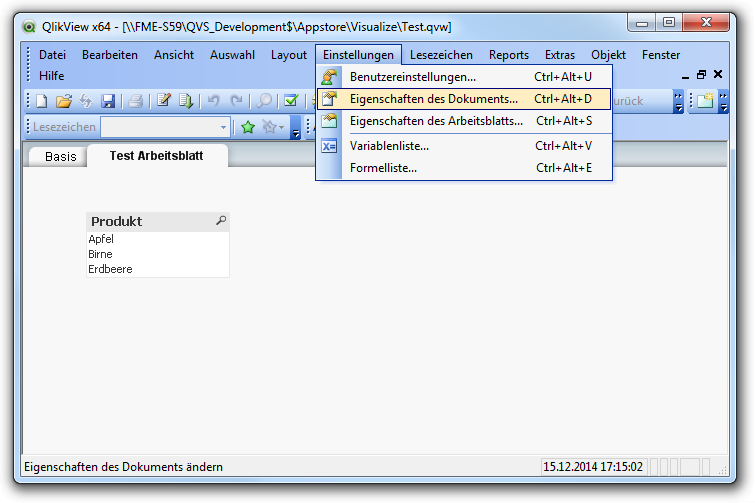
\includegraphics[width=1.00\textwidth]{img/DocumentExtensionListe/EigenschaftendesDokumentes.png}
	\caption[Öffnen der Eigenschaften des Dokumentes in QlikView]{Öffnen der Eigenschaften des Dokumentes in QlikView, \\Quelle: Eigene Abbildung}
	\label{fig:EigenschaftendesDokumentes}
\end{figure}


\begin{figure}[htbp]
	\centering
		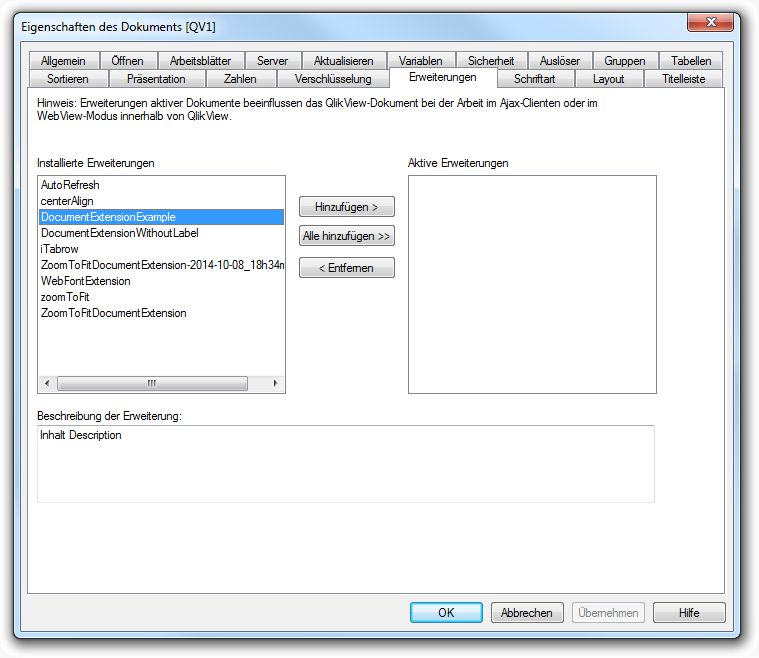
\includegraphics[width=1.00\textwidth]{./img/DocumentExtensionListe/DocumentExtensionListe.png}
	\caption[Liste der verfügbaren Document Extensions]{Liste der verfügbaren Document Extensions zum Hinzufügen zum QlikView-Dokument, Quelle: Eigene Abbildung}
	\label{fig:DocumentExtensionListe}
\end{figure}
% Beispiel Dateien erstellen
% Aus aktuellem Beispiel die Platzhalter rausnehmen




\begin{figure}[htbp]
	\centering
		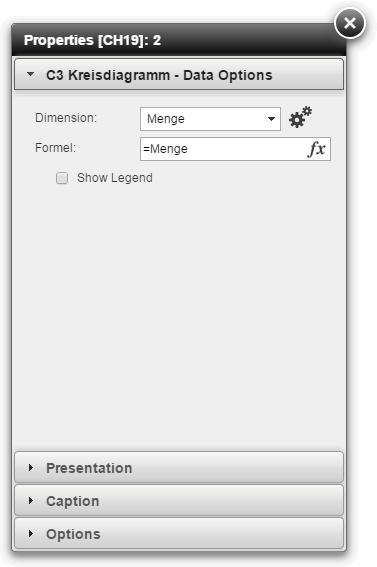
\includegraphics[width=0.70\textwidth]{img/QvPropDialog/C3KreisdiagrammDialog.png}
	\caption[QlikView JavaScript C3 Kreisdiagramm Konfigurationsdialog]{Screenshot des QlikView JavaScript C3 Kreisdiagramm Konfigurationsdialoges, Quelle: Eigene Abbildung}
	\label{fig:QlikViewC3KreisdiagrammDialogScreenshot}
\end{figure}




\begin{figure}[htbp]
	\centering
		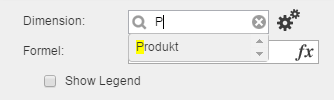
\includegraphics[width=0.60\textwidth]{img/QvPropDialog/DimensionAutomatischeVervollstaendigung.png}
		\caption[Automatischen Vervollständigung der Dimension]{Screenshot der automatischen Vervollständigung der Dimension, \\Quelle: Eigene Abbildung}
	\label{fig:DimensionAutomatischeVervollstaendigung}
\end{figure}



\begin{figure}[htbp]
	\centering
		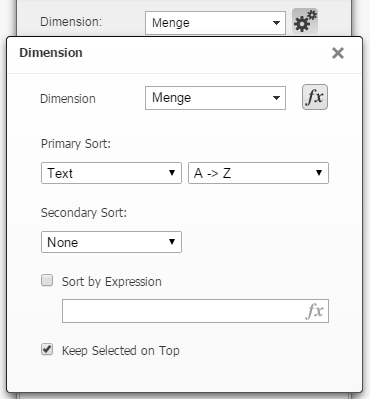
\includegraphics[width=0.70\textwidth]{img/QvPropDialog/DimensionSortierung.png}
	\caption[QlikView JavaScript C3 Kreisdiagramm Sortierungskonfiguration]{QlikView JavaScript C3 Kreisdiagramm Sortierungskonfiguration, \\Quelle: Eigene Abbildung}
	\label{fig:DimensionSortierung}
\end{figure}

\newpage
\subsection{Properties.qvpp-Datei des C3Kreisdiagramm Extension Objects} 
\label{lab:QlikViewJavascriptC3KreisdiagrammKonfigurationsdialog} 

\begin{listing}[htbp]
\begin{minted}[mathescape,
               linenos,
               numbersep=5pt,
							fontsize=\small,
               gobble=0,
               frame=lines,
							 fontsize=\scriptsize,
               framesep=2mm]{html}
<div class="ToolWindow-MainBody" avq="foldOutMenu:."
  style="overflow: visible !important; float: left;">
  <div class="prop-accordion" avq="accordion:.">
    <h3 class="prop-h3 accordion-shadow">
      <a href="#"> C3 Kreisdiagramm - Data Options </a>
    </h3>
    <div class="prop-grid_container accordion-shadow-enabler"
      style="overflow:auto;">
      <div class="prop-grid_clear 
        prop-grid_top-vertical-spacer-12px prop-grid_last"></div>
      <div class='prop-grid_clear prop-grid_prepend-1 prop-grid_span-5'
        avq='prop_label'>Dimension:</div>
      <div class='prop-grid_span-10 prop-grid_last'>
        <div class='prop-grid_span-7' 
          avq='prop_dynamicDropdown:.Chart.Dimension.0.Field'></div>
        <div class='prop-width-28px' propicontype='tool'
          avq='prop_dlgbuttonjqui:.Chart.Dimension.0:ExtensionDimDialog.qvpp'>
        </div>
      </div><br />
      <div class='prop-grid_clear prop-grid_prepend-1 prop-grid_span-5'
        avq='prop_label'>Formel:</div>
      <div class='prop-grid_span-10 prop-grid_last'>
        <div class='prop-grid_span-7 prop-grid_last'
          style='width:94%;' 
          avq='prop_editexpression:.Chart.Expression.0.0.Definition'></div>
      </div><br />
      <div class='prop-grid_clear prop-grid_prepend-1'>
        <div class='prop-grid_span-1'></div>
        <div class='prop-grid_span-1' 
          avq='prop_checkbox:.Chart.Text.0.Content'></div>
        <div class='prop-grid_span-7 prop-grid_last'
          avq='prop_label'>Zeige Legende:</div>
      </div>
    </div>
    <h3 class="prop-h3 accordion-shadow" avq="activeAccordionHeader:.:GenericPresentationFoldout.qvpp">
      <a href="#">Presentation</a></h3>
    <div class="prop-grid_container accordion-shadow-enabler" style="height:300px;"
      avq="panel::Layout.qvpp"></div>
    <h3 class="prop-h3 accordion-shadow" avq="activeAccordionHeader::PropertiesCaptionFoldout.qvpp">
      <a href="#">Caption</a></h3>
    <div class="prop-grid_container accordion-shadow-enabler" avq="panel::Caption.qvpp"></div>
      <h3 class="prop-h3 accordion-shadow" avq="activeAccordionHeader:.:PropertiesOptionsFoldout.qvpp">
      <a href="#">Options</a></h3>
    <div class="prop-grid_container accordion-shadow-enabler" avq="panel::Options.qvpp"></div>
  </div><span class="bottom-gap"></span>
</div>
\end{minted}
\caption[\textit{Properties.qvpp}-Datei des QlikView C3Kreisdiagramm Extension Objects]{\textit{Properties.qvpp}-Datei des QlikView C3Kreisdiagramm Extension Objects, Quellcode\textbackslash{}JavaScript\textbackslash{}QlikView\textbackslash{}C3Kreisdiagramm\textbackslash{}Properties.qvpp, \\Quelle: Eigenes Listing}
\label{lst:QlikViewJavascriptC3KreisdiagrammSkript}
\end{listing}

\newpage
\subsection{Screenshots von Qlik Sense} 
\label{lab:ScreenshotsVonQlikSense} 

\begin{figure}[htbp]
	\centering
		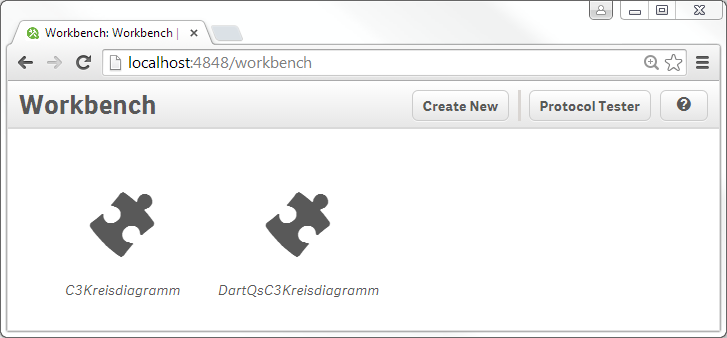
\includegraphics[width=1.00\textwidth]{img/SenseScreenshots/Workbench.PNG}
	\caption[Screenshot der Qlik Sense Workbench]{Screenshot der Qlik Sense Workbench, Quelle: Eigene Abbildung}
	\label{fig:Workbench}
\end{figure}

\begin{figure}[htbp]
	\centering
		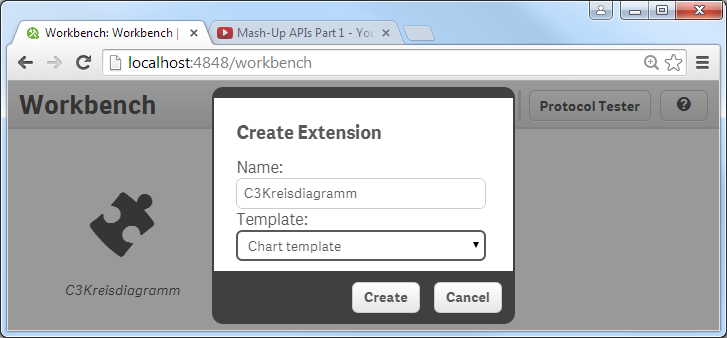
\includegraphics[width=1.00\textwidth]{img/SenseScreenshots/WorkbenchCreateNew.PNG}
	\caption[Screenshot des Dialoges zur Erstellung eines Qlik Sense Extension Objects]{Screenshot des Dialoges zur Erstellung eines Qlik Sense Extension Objects, \\Quelle: Eigene Abbildung}
	\label{fig:WorkbenchCreateNew}
\end{figure}

\newpage

\begin{figure}[htbp]
	\centering
		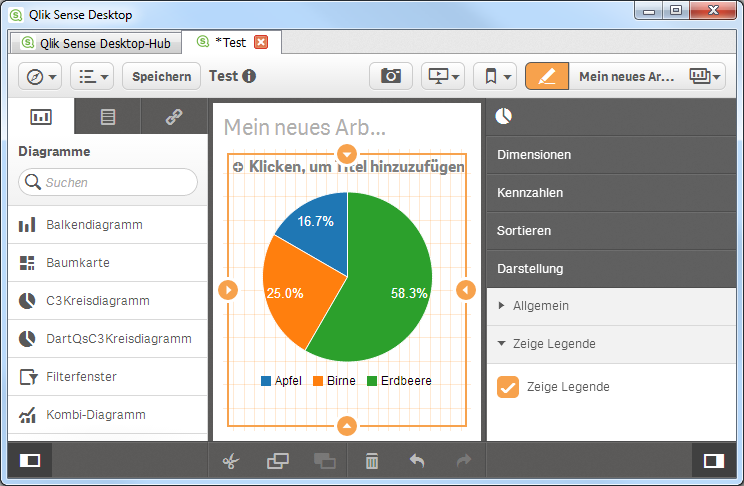
\includegraphics[width=1.00\textwidth]{img/SenseScreenshots/ArbeitsblattQlikSense.PNG}
	\caption[Screenshot des C3Kreisdiagramms in einem Qlik Sense Arbeitsblatt]{Screenshot eines Qlik Sense Arbeitsblattes mit der hinzugefügten Erweiterung C3Kreisdiagramm - mitte - und eingeblendetem \textit{accordion} zur Konfiguration - rechts, Quelle: Eigene Abbildung}
	\label{fig:ArbeitsblattQlikSense}
\end{figure}


\newpage
\subsection{Beispiel-Screenshot der DownloadArbeitsblattAlsPng-Erweiterung} 
\label{lab:BeispielScreenshotDownloadArbeitsblattAlsPng} 



\begin{figure}[htbp]
	\centering
		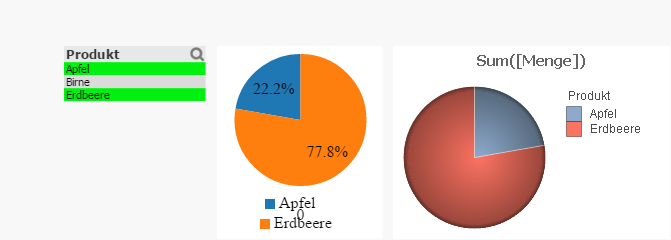
\includegraphics[width=1.00\textwidth]{img/ScreenshotSheet/ScreenshotSheet.png}
	\caption[Durch die Erweiterung DownloadArbeitsblattAlsPng heruntergeladener Screenshot]{Durch die Erweiterung DownloadArbeitsblattAlsPng heruntergeladener Screenshot, \\Quelle: Eigene Abbildung}
	\label{fig:ScreenshotSheet}
\end{figure}


\newpage
\subsection{initialProperties für ein Qlik Sense Extension Object in Dart-Syntax} 
\label{lab:initialPropertiesQlikSenseExtensionObjectDartSyntax} 

Im Listing \ref{lst:initialPropertiesQlikSenseExtensionObjectDartSyntax} ist die testweise Portierung der \textit{initialProperties.js}-Datei zu sehen. In den Zeilen 4, 5 und 6 ist die Erstellung von JavaScript-Proxy-Objekten mithilfe des Konstruktors \textit{JsObject.jsify} zu sehen. Dies es notwendig, denn in Dart erstellte Kollektionen sind nicht mit JavaScript kompatibel, auch wenn es sich um leere Listen wie in den Zeilen 4 und 5 handelt. Daher müssen sie konvertiert werden.

\begin{listing}[htbp]
\begin{minted}[mathescape,
               linenos,
               numbersep=5pt,
               gobble=0,
               frame=lines,
							fontsize=\footnotesize,
               framesep=2mm]{html}
'initialProperties': {
  'version': 1.0,
  'qHyperCubeDef': {
    'qDimensions': new JsObject.jsify([]),
    'qMeasures': new JsObject.jsify([]),
    'qInitialDataFetch': new JsObject.jsify([{
      'qWidth': 10,
      'qHeight': 50
    }])
  }
}
\end{minted}
\caption[\textit{initialProperties} für ein Qlik Sense Extension Object in Dart-Syntax]{\textit{initialProperties} für ein Qlik Sense Extension Object in Dart-Syntax, \\Quelle: Eigenes Listing}
\label{lst:initialPropertiesQlikSenseExtensionObjectDartSyntax}
\end{listing}


\newpage
\subsection{Klassendiagramm des Projektes qlikview""\_qlik""\_sense""\_extensions} 
\label{lab:KlassendiagrammDerKlassenbibliothek} 

\begin{figure}[htbp]
	\centering
		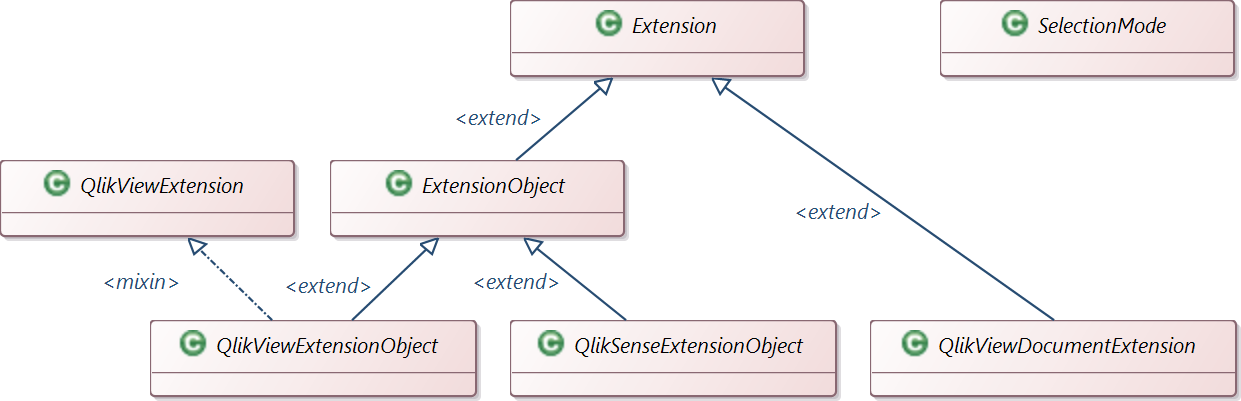
\includegraphics[width=1.00\textwidth]{img/Klassendiagramm/Klassendiagramm.png}
	\caption[Klassendiagramm der Klassenbibliothek \textit{qlikview\_qlik\_sense\_extensions}]{Klassendiagramm der Klassenbibliothek \textit{qlikview\_qlik\_sense\_extensions}, Quelle: Eigene Abbildung}
	\label{fig:Klassendiagramm}
\end{figure}


\newpage
\subsection{Listings zu source maps} 
\label{lab:ListingsZuSourceMaps} 

\begin{listing}[htbp]
\begin{minted}[mathescape,
               linenos,
               numbersep=5pt,
               gobble=0,
               frame=lines,
							fontsize=\footnotesize,
               framesep=2mm]{Bash}
# sourceMappingURL=main.dart.js.map
\end{minted}
\caption[Beispiel für einen Verweis auf eine source map]{Beispiel für einen Verweis auf eine source map, Quelle: Eigenes Listing}
\label{lst:BeispielVerweisSourceMap}
\end{listing}

\begin{listing}[htbp]
\begin{minted}[mathescape,
               linenos,
               numbersep=5pt,
               gobble=0,
               frame=lines,
							fontsize=\scriptsize,
               framesep=2mm]{javascript}
{
  "version": 3,
  "file": "main.dart.js",
  "sourceRoot": "",
  "sources": ["packages/$sdk/lib/_internal/compiler/js_lib/interceptors.dart" 
             ,"packages/$sdk/lib/_internal/compiler/js_lib/js_array.dart" 
             ,"packages/$sdk/lib/collection/list.dart" 
             ,"packages/$sdk/lib/internal/iterable.dart" 
             ,"packages/$sdk/lib/_internal/compiler/js_lib/js_number.dart" 
             ,"packages/$sdk/lib/_internal/compiler/js_lib/js_string.dart" 
             ,"packages/$sdk/lib/_internal/compiler/js_lib/isolate_helper.dart" 
             ,"packages/$sdk/lib/collection/queue.dart" 
             ,"packages/$sdk/lib/_internal/compiler/js_lib/js_helper.dart" 
             ,"packages/$sdk/lib/_internal/compiler/js_lib/collection_patch.dart" 
             ,"packages/$sdk/lib/collection/iterable.dart" 
             ,"packages/$sdk/lib/async/timer.dart" 
             ,"packages/$sdk/lib/_internal/compiler/js_lib/native_helper.dart" 
             ,"packages/$sdk/lib/_internal/compiler/js_lib/js_rti.dart" 
             ,"packages/$sdk/lib/internal/lists.dart" 
             ,"packages/$sdk/lib/internal/symbol.dart" 
             ,"packages/$sdk/lib/_internal/compiler/js_lib/js_names.dart" 
             ,"packages/$sdk/lib/_internal/compiler/js_lib/async_patch.dart" 
             ,"packages/$sdk/lib/async/async_error.dart" 
             ,"packages/$sdk/lib/async/future.dart" 
             ,"packages/$sdk/lib/async/future_impl.dart" 
             ,"packages/$sdk/lib/async/schedule_microtask.dart" 
             ,"packages/$sdk/lib/async/zone.dart" 
             ,"packages/$sdk/lib/core/duration.dart" 
             ,"packages/$sdk/lib/collection/hash_map.dart" 
             ,"packages/$sdk/lib/_internal/compiler/js_lib/core_patch.dart" 
             ,"packages/$sdk/lib/collection/maps.dart" 
             ,"packages/$sdk/lib/collection/set.dart" 
             ,"packages/$sdk/lib/core/errors.dart" 
             ,"packages/$sdk/lib/core/exceptions.dart" 
             ,"packages/$sdk/lib/core/print.dart" 
             ,"packages/$sdk/lib/_internal/compiler/js_lib/internal_patch.dart" 
             ,"packages/$sdk/lib/core/expando.dart" 
             ,"packages/$sdk/lib/core/null.dart" 
             ,"packages/$sdk/lib/core/object.dart" 
             ,"packages/$sdk/lib/core/string_buffer.dart" 
             ,"packages/$sdk/lib/html/dart2js/html_dart2js.dart" 
             ,"packages/$sdk/lib/_internal/compiler/js_lib/native_typed_data.dart" 
             ,"packages/$sdk/lib/_internal/compiler/js_lib/js_primitives.dart" 
             ,"main.dart"],
\end{minted}
\caption[Auszug einer formatierten source map]{Auszug einer formatierten source map, Quelle: Eigenes Listing}
\label{lst:AuszugEinerFormatiertenSourceMap}
\end{listing}


\newpage
\subsection{Fehlerhafte Verwendung der QlikView Ajax API} 
\label{lab:FehlerhafteVerwendungDerQlikViewAjaxAPI} 

Im Listing \ref{lst:AnimatedScatterChartScriptJsDatei} ist ein Auszug aus der \textit{Script.js}-Datei der QlikView Extension \textit{Animated Scatter Chart} zu sehen. In der Zeile 3 wird der Funktion \textit{AddExtension} die Callback-Funktion übergeben, welche unter anderem auch den Aufruf der Funktionen \textit{LoadCSS} in Zeile 30 und \textit{LoadExtensionScripts} in Zeile 37 enthält. Doch da die Callback-Funktion bei jedem Zeichnen aufgerufen wird, werden diese Ressourcen auch bei jedem Zeichnen erneut dem \textit{head}-Element des Dokuments hinzugefügt.

\begin{listing}[htbp]
\begin{minted}[mathescape,
               linenos,
               numbersep=5pt,
							fontsize=\footnotesize,
               gobble=0,
               frame=lines,
               framesep=2mm]{javascript}
function D3AnimatedScatterChart_Init() {

    Qva.AddExtension("D3AnimatedScatterChart",
        function() {

          ConsoleClear();
          fixSelectBox();

          var _this = this;
          _this.ExtSettings = {};
          _this.ExtSettings.ExtensionName = 'D3AnimatedScatterChart';
          _this.ExtData = {};

          // Base Url for CSS Files
          _this.ExtSettings.LoadUrl = Qva.Remote + (Qva.Remote.indexOf('?') >=
            0 ? '&' : '?') + 'public=only' + '&name=';

          //Todo: Can be removed in final version
          _this.ExtSettings.DataFile = Qva.Remote + (Qva.Remote.indexOf('?') >=
              0 ? '&' : '?') + 'public=only' +
            '&name=Extensions/D3AnimatedScatterChart/lib/data/nations.json';
          _this.ExtSettings.DataFile_Full = Qva.Remote + (Qva.Remote.indexOf(
              '?') >= 0 ? '&' : '?') + 'public=only' +
            '&name=Extensions/D3AnimatedScatterChart/lib/data/nations_full.json';

          var cssFiles = [];
          cssFiles.push('Extensions/' + _this.ExtSettings.ExtensionName +
            '/lib/css/style.css');
          for (var i = 0; i < cssFiles.length; i++) {
            Qva.LoadCSS(_this.ExtSettings.LoadUrl + cssFiles[i]);
          }

          var jsFiles = [];
          //http://d3js.org/d3.v2.js?2.8.1
          jsFiles.push('Extensions/' + _this.ExtSettings.ExtensionName +
            '/lib/js/d3_v2.js');
          Qv.LoadExtensionScripts(jsFiles, function() {
\end{minted}
\caption[Formatierter Auszug der \textit{Script.js}-Datei des Animated Scatter Chart]{Formatierter Auszug der \textit{Script.js}-Datei des Animated Scatter Chart, \\Quelle: \cite{QlikViewExtensionAnimatedScatterChartSourceCode}}
\label{lst:AnimatedScatterChartScriptJsDatei}
\end{listing}

Die Abbildung \ref{fig:endOfHead} zeigt, dass diese Ressourcen tatsächlich mehrfach im \textit{head}-element des Dokuments auftauchen. In Abbildung \ref{fig:Sources} ist darüber hinaus zu sehen, dass diese Dateien bei deaktiviertem Browsercache sogar mehrfach vom Server angefragt und erneut heruntergeladen werden.

\begin{figure}[htbp]
	\centering
		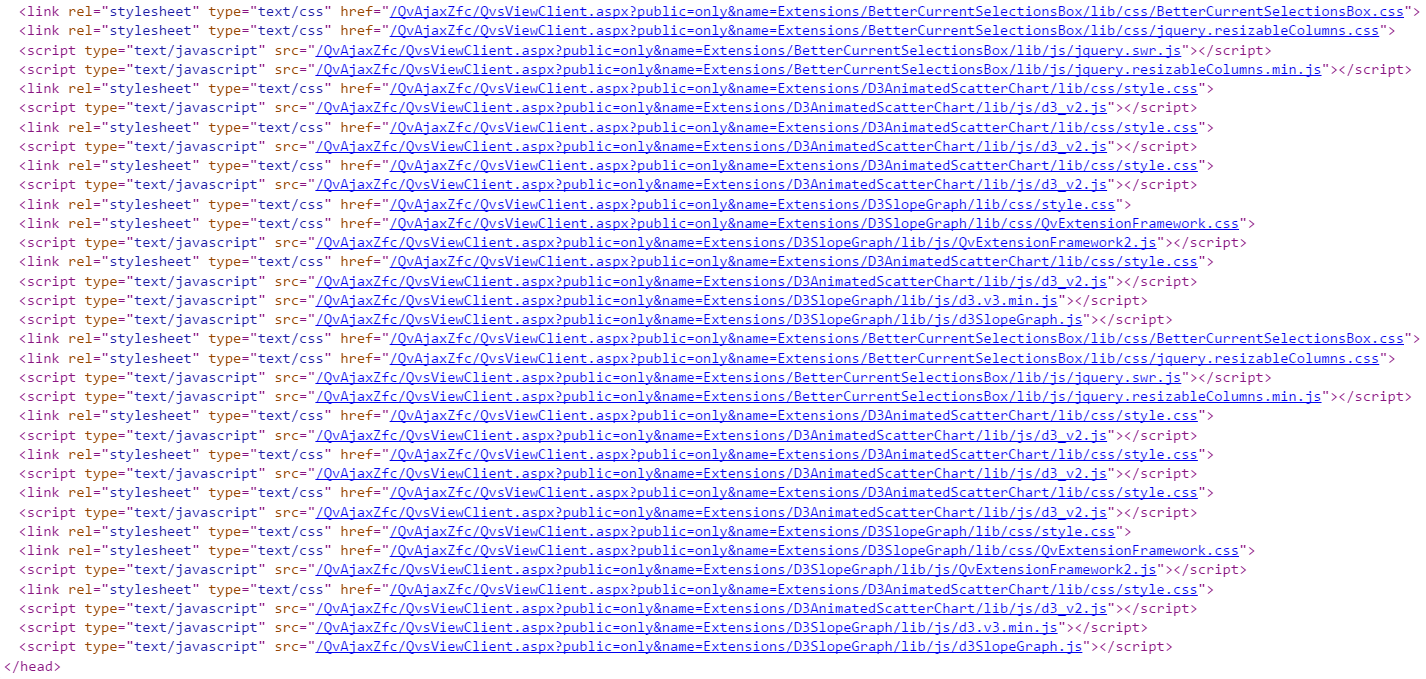
\includegraphics[width=1.00\textwidth]{img/headRudundant/endOfHead.PNG}
	\caption[Redundante Einträge im \textit{head}-Element des Dokuments]{Durch fehlerhafte Verwendung der QlikView Ajax API tauchen redundante Einträge im \textit{head}-Element des Dokuments auf, \\Quelle: Eigene Abbildung}
	\label{fig:endOfHead}
\end{figure}

\begin{figure}[htbp]
	\centering
		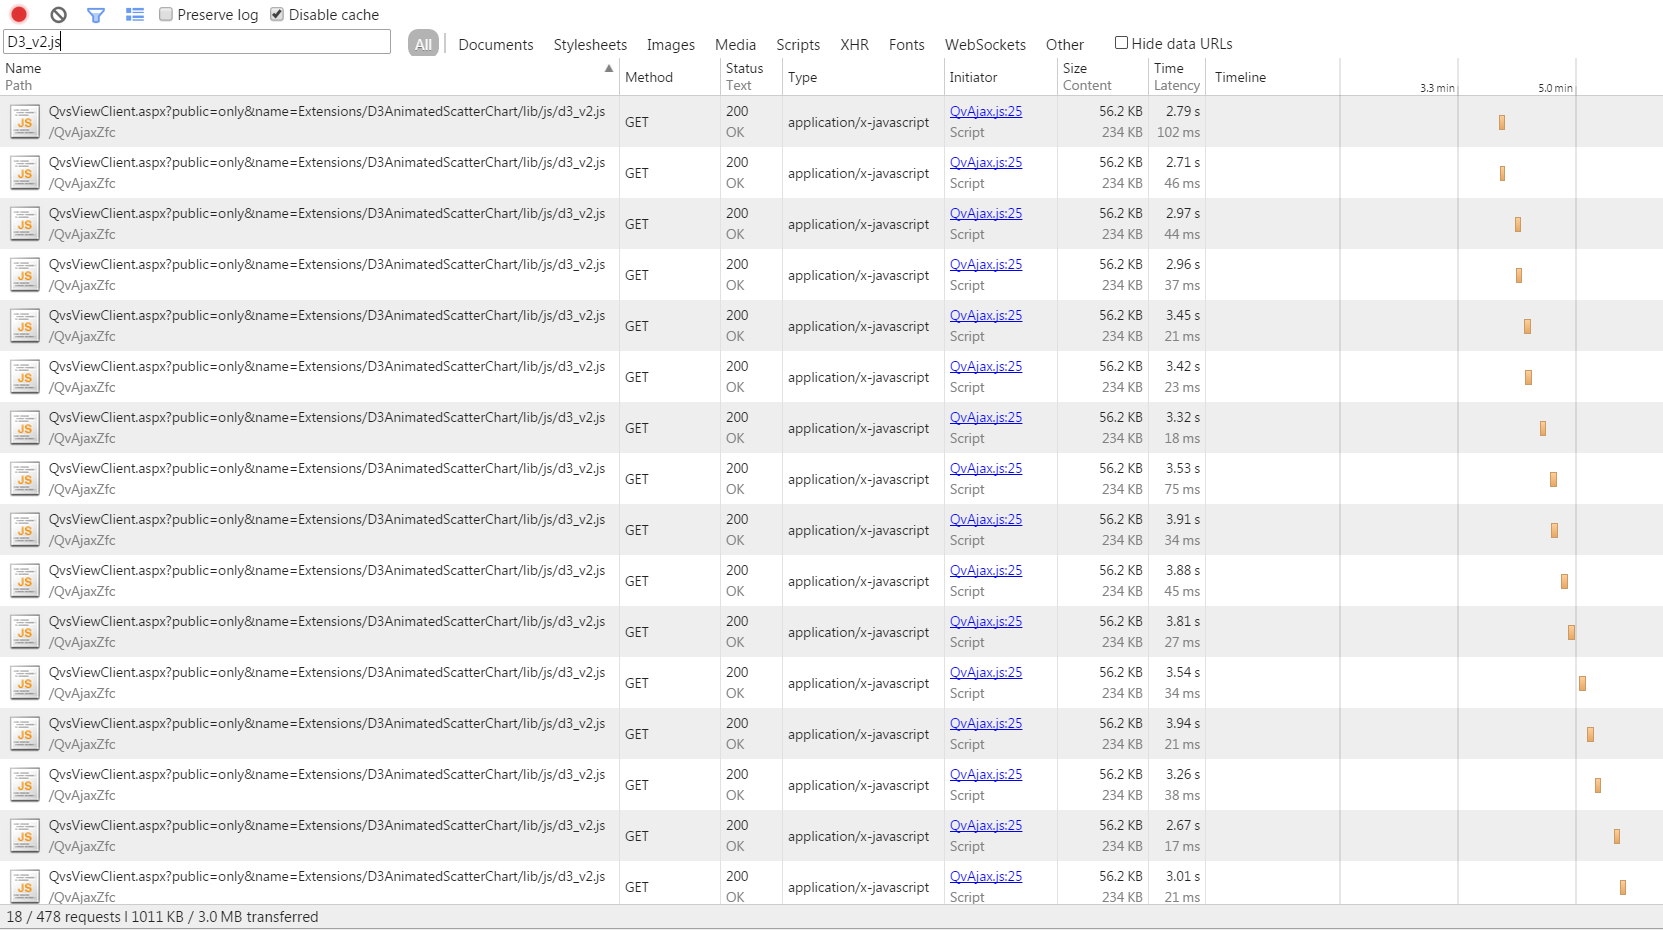
\includegraphics[width=1.00\textwidth]{img/headRudundant/Sources.png}
	\caption[Mehrfaches Herunterladen derselben Datei.]{Die Filterung nach der Bibliothek d3\_v2 zeigt, dass bei deaktiviertem Browsercache dieselbe Datei mehrfach heruntergeladen wird, \\Quelle: Eigene Abbildung}
	\label{fig:Sources}
\end{figure}


\newpage
\subsection{Abbildungen zur erleichterten Entwicklung mit Dart} 
\label{lab:AbbildungenZurErleichtertenEntwicklungVonErweiterungenMitDart}

Mit einem Rechtsklick im Editor öffnet sich ein Kontextmenü, in dem unter anderem der Eintrag \textit{Quick Fix} verfügbar ist. Alternativ kann die Funktion mit der Tastenkombination Steuerung + 1 aufgerufen werden. Bei Fehlermeldungen und Warnungen bietet sie Lösungsvorschläge an und generiert automatisch den passenden Code.

\begin{figure}[htbp]
	\centering
		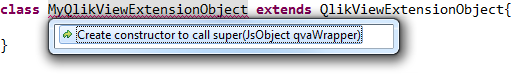
\includegraphics[width=1.00\textwidth]{img/HilfeDurchEditor/implConstr.png}
	\caption[Vorschlag zur automatischen Implementierung des Konstruktors]{Vorschlag zur automatischen Implementierung des Konstruktors, \\Quelle: Eigene Abbildung}
	\label{fig:implConstr}
\end{figure}

In Abbildung \ref{fig:implConstr} ist zu sehen, dass der Klasse \textit{MyQlikViewExtensionObject} der Aufruf des Konstruktors der Basisklasse fehlt. Die automatische Implementierung des Konstruktors wird angeboten. Anschließend wird eine Warnung ausgegeben, dass zwei Schnittstellen in der konkreten Klasse noch immer nicht implementiert sind.

\begin{figure}[htbp]
	\centering
		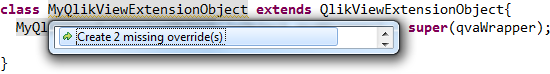
\includegraphics[width=1.00\textwidth]{img/HilfeDurchEditor/implOverride.png}
	\caption[Vorschlag zur automatischen Implementierung der fehlenden Schnittstellen]{Vorschlag zur automatischen Implementierung der fehlenden Schnittstellen, \\Quelle: Eigene Abbildung}
	\label{fig:implOverride}
\end{figure}

Abbildung \ref{fig:implOverride} zeigt, dass in diesem Fall die Generierung der Methodenköpfe angeboten wird. Die vollständige Struktur der Klasse ist in Abbildung \ref{fig:complete} zu sehen. Nach dem Eingeben von \textit{this.} erscheint eine Liste von Vorschlägen für automatische Vervollständigungen. In der Liste sind lediglich die im Kontext sichtbaren Felder und Methoden aufgeführt. Diese Hilfestellungen erleichtern die Einarbeitung, beschleunigen die Entwicklung und beugen Fehlern vor.

\begin{figure}[htbp]
	\centering
		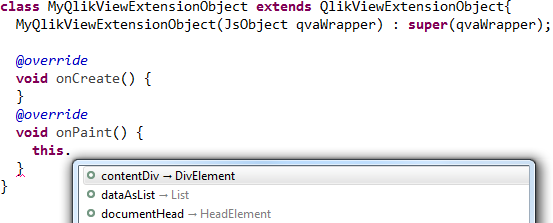
\includegraphics[width=1.00\textwidth]{img/HilfeDurchEditor/complete.png}
	\caption[Automatische Vervollständigung der möglichen Felder und Methoden]{Automatische Vervollständigung der möglichen Felder und Methoden, Quelle: Eigene Abbildung}
	\label{fig:complete}
\end{figure}



\end{appendix} 


%Hiermit versichere ich, dass ich die vorliegende Arbeit selbstständig verfasst und keine anderen als
%die angegebenen Quellen und Hilfsmittel benutzt habe. Alle Ausführungen, die fremden Quellen
%wörtlich oder sinngemäß entnommen wurden, sind kenntlich gemacht. Die Arbeit war in gleicher
%oder ähnlicher Form noch nicht Bestandteil einer Studien- oder Prüfungsleistung.
%Braunschweig, den 16.12.2014
%Alexander Johr
%\chapter{Eidesstattliche Erklärung}
\newpage
\mbox{}
\newpage


\clearpage
\section*{Eidesstattliche Erklärung}
\addcontentsline{toc}{section}{Eidesstattliche Erklärung}%\addtocontents{toc}{\vfill}
Ich erkläre, dass ich meine Bachelor-Arbeit "`Entwicklung von Extension Objects sowie Document Extensions für QlikView 11 und Qlik Sense mit Dart"' selbstständig und ohne Benutzung anderer als der angegebenen Hilfsmittel angefertigt habe und dass ich alle Stellen, die ich wörtlich oder sinngemäß aus Veröffentlichungen entnommen habe, als solche kenntlich gemacht habe. Die Arbeit hat bisher in gleicher oder ähnlicher Form oder auszugsweise noch keiner Prüfungsbehörde vorgelegen.\\\\

Ich versichere, dass die eingereichte schriftliche Fassung der auf dem beigefügten Medium gespeicherten Fassung entspricht.
\\\\\\
\noindent Braunschweig, den 14.02.2015
\begin{flushright}
$\overline{~~~~~~~~~\mbox{Alexander Johr}~~~~~~~~~}$
\end{flushright}

\newpage
\mbox{}

\end{document}
